\chapter{Revisão bibliográfica}

Esse capítulo é uma revisão da literatura em modelagem geológica automática e avaliação de incerteza em modelos geológicos com ênfase no uso de funções distância assinaladas.

\section{Modelagem geológica determinística}

A dispendiosidade na construção e a inflexibilidade dos modelos explícitos impulsionaram o desenvolvimento de técnicas de modelagem geológica automáticas. As técnicas determinísticas geram apenas um único modelo, consequentemente, não possibilitando a avaliação da incerteza associada ao modelo geológico. 

Métodos matemáticos menos sofisticados, como o vizinho mais próximo podem ser utilizados na criação automática de modelos geológicos determinísticos. Esse algoritmo constrói ao redor de cada amostra sua área de influência, ou volume de influência em três dimensões. A toda a área de influência é atribuída a categoria, ou litologia, correspondente àquela amostra. 

Métodos baseados em aprendizado de máquina também podem ser utilizados. \citeonline{smirnoff2008support} propuseram o uso de máquina de vetores de suporte (\textit{support vector machine}) para a criação de modelos geológicos determinísticos multi-categóricos a partir de amostras esparsas de diferentes origens.

Métodos geoestatísticos também têm aplicação na criação de modelos geológicos de forma automática, a krigagem dos indicadores \cite{alabert1987stochastic} consiste na geração de uma distribuição acumulada de probabilidades a partir da transformação não linear dos dados. Para variáveis categóricas, é possível estimar diretamente a probabilidade de cada local não amostrado pertencer a cada uma das diferentes litologias do depósito mineral. A partir das probabilidades um modelo geológico pode ser criado.
 
A família de métodos ditos métodos implícitos compreendem técnicas importadas da computação gráfica. O uso da modelagem implícita foi introduzida no campo da computação gráfica para a geração de objetos de diferentes geometrias e complexidades por  \citeonline{bloomenthal1997introduction}. A ideia geral é usar uma função implícita para demarcar regiões de diferentes formas e extensões no espaço. \citeonline{cowan2002rapid} e \citeonline{cowan2003practical} popularizaram a modelagem implícita no contexto geológico, baseados no trabalho de \citeonline{savchenko}, que modela objetos tridimensionais a partir de dados esparsos interpolando uma função volume.

Modelos geológicos implícitos são criados a partir de dados esparsos, geralmente, dados categóricos (\autoref{imp_mod} (a)). Os pontos amostrais podem ser usados para derivar uma função implícita que fornece uma representação matemática contínua de um atributo através de um volume, um campo escalar ou modelo implícito (\autoref{imp_mod} (b)). Modelos implícitos contém um número infinito de isosuperfícies. Para visualizar o modelo geológico uma isosuperfície específica deve ser extraída do modelo e mostrada no espaço tridimensional (geralmente a isosuperfície zero), $f(x,y,z)=s$, onde $s$ é o valor de interesse no campo escalar (\autoref{imp_mod} (c)). A localização dessa superfície é conhecida implicitamente como função da localização no domínio \cite{martin2017implicitmodeling}. 

\begin{figure}[H]
    \centering
	\caption{\label{imp_mod}Ilustração esquemática da modelagem geológica implícita.}
	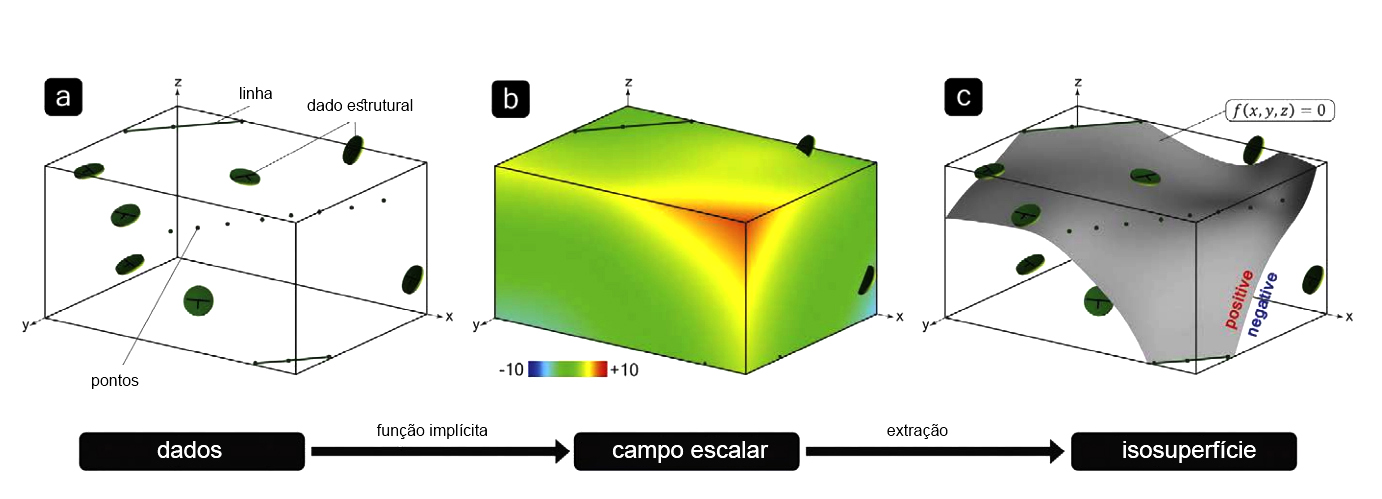
\includegraphics[width=\textwidth]{capitulo_2/imagens/implicit_modelig_pt_1.jpg}
	\legend{Modificado de \cite{aillerespresentation}}
\end{figure}

Diferentes tipos de dados amostrais podem ser usados para derivar diferentes funções volume na modelagem implícita. \citeonline{mallet2004space} propõe uma função volumétrica cronológica, levando em consideração a posição estratigráfica das diferentes unidades geológicas, enquanto \citeonline{lajaunie1997foliation, chiles2004modelling, calcagno2008geological} usam co-krigagem de incrementos em um campo potencial, omitindo a função volume. O procedimento não é simples já que a covariância do campo potencial é particularmente difícil de inferir uma vez que não há \textit{hard data} de campo potencial disponível.

A função volume mais comumente utilizada é a função distância assinalada \cite{osherlevelsetmethods}. A aplicação dessa metodologia é encontrada por toda a literatura de interpolação de dados esparsos, uma das aplicações é a reconstrução de superfícies a partir de escaneamento. Na modelagem geológica, a metodologia é competente em capturar a geometria e extensão de corpos geológicos e tem sido aplicada com sucesso há mais de uma década na exploração mineral tendo ganhado espaço em diferentes \textit{softwares} comerciais. Para bancos de dados pontuais, que representam a posição  de diferentes litologias no espaço, o uso das funções distância assinaladas torna os processos de interpretação, cálculo, modelagem, modificação do modelo de acordo com a interpretação dos geomodeladores e avaliação da incerteza diretos e rápidos. Além disso, informações a respeito da orientação das unidades geológicas (dados estruturais) podem ser imputada como restrição na criação do modelo geológico \cite{martin2017implicitmodeling}.

As próximas seções trazem uma revisão bibliográfica extensiva da modelagem geológica com funções distância assinaladas.

\subsection{Modelagem geológica com funções distância assinaladas}

Para  ilustrar a metodologia será utilizado o \textit{dataset} \textit{Swiss Jura} \cite{goovaerts1997geostatistics}. O \textit{dataset} compreende 259 amostras da propriedade \textit{rock type} (RT). Um mapa com a localização das amostras é mostrado na \autoref{jura_pontos}.

A variável RT possui cinco categorias: \textit{Argovian; Kimmeridgian; Sequian;
Portlandian; e Quartenary}. A área é coberta parcialmente com amostras uniformemente espaçadas, algumas áreas são densamente amostradas com agrupamento adicional de amostras.

\begin{figure}[H]
	\centering
	\caption{\label{jura_pontos}Mapa de localização das 259 amostras do \textit{dataset} \textit{Swiss Jura}.}
	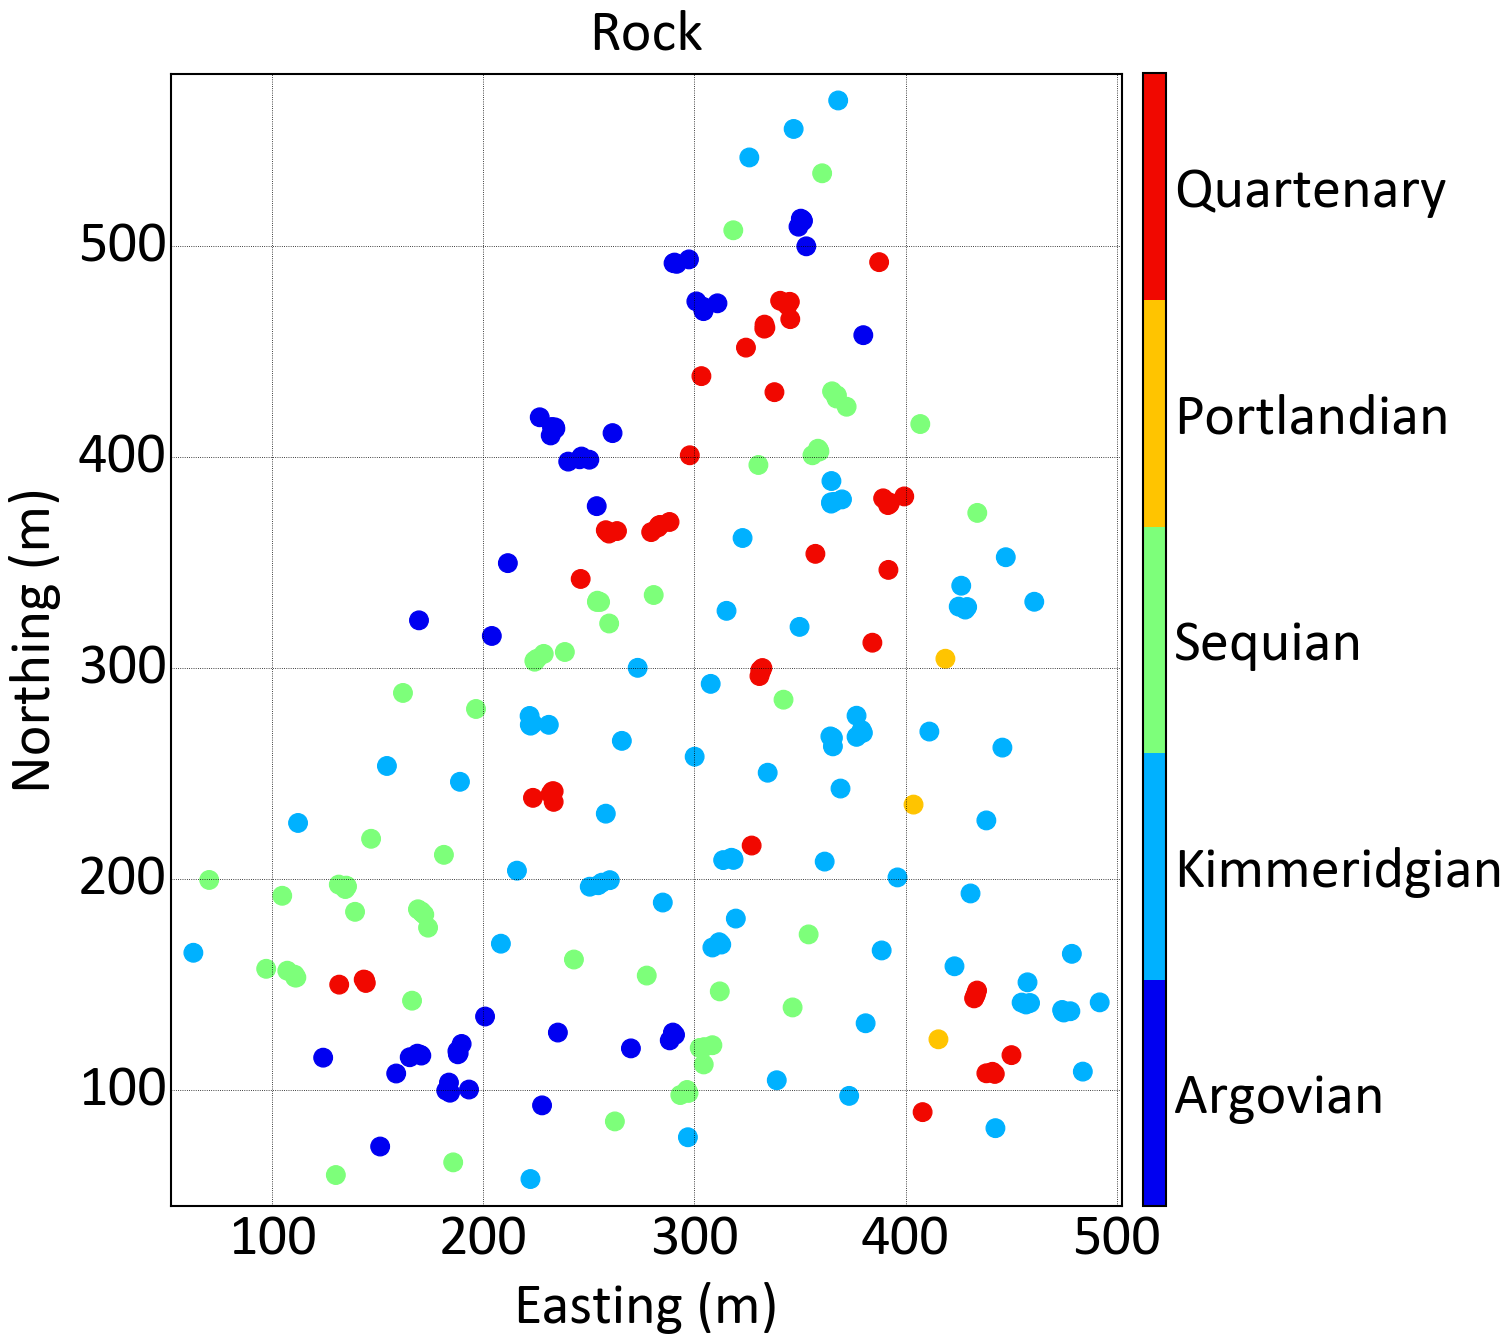
\includegraphics[width=0.6\textwidth]{capitulo_2/imagens/points.png}
\end{figure}

\subsubsection{Cálculo das distâncias assinaladas}

O primeiro passo no cálculo das distâncias assinaladas é transformar as amostras ${z(u_\alpha),\alpha=1,...,n}$ em indicadores binários de acordo com a \autoref{eq_ind}, especificando se a amostra pertence ou não ao domínio $k$ que está sendo modelado.

\begin{equation}
	i_k(u_\alpha)=\begin{cases}
	1,\:\textrm{se}\:z(u_\alpha)\:\textrm{se pertence ao domínio $k$}\\
	0,\:\textrm{se}\:z(u_\alpha)\:\textrm{caso contrário}\end{cases}
    \label{eq_ind}
\end{equation}

Como exemplo será utilizada a categoria Quaternary do \textit{Swiss Jura}. A \autoref{ind_5} mostra as amostras do \textit{Swiss Jura} transformadas em indicadores para essa categoria.

\begin{figure}[H]
	\centering
	\caption{\label{ind_5}Mapa de localização das 259 amostras dos indicadores para a categoria Quaternary do \textit{dataset} \textit{Swiss Jura}.}
	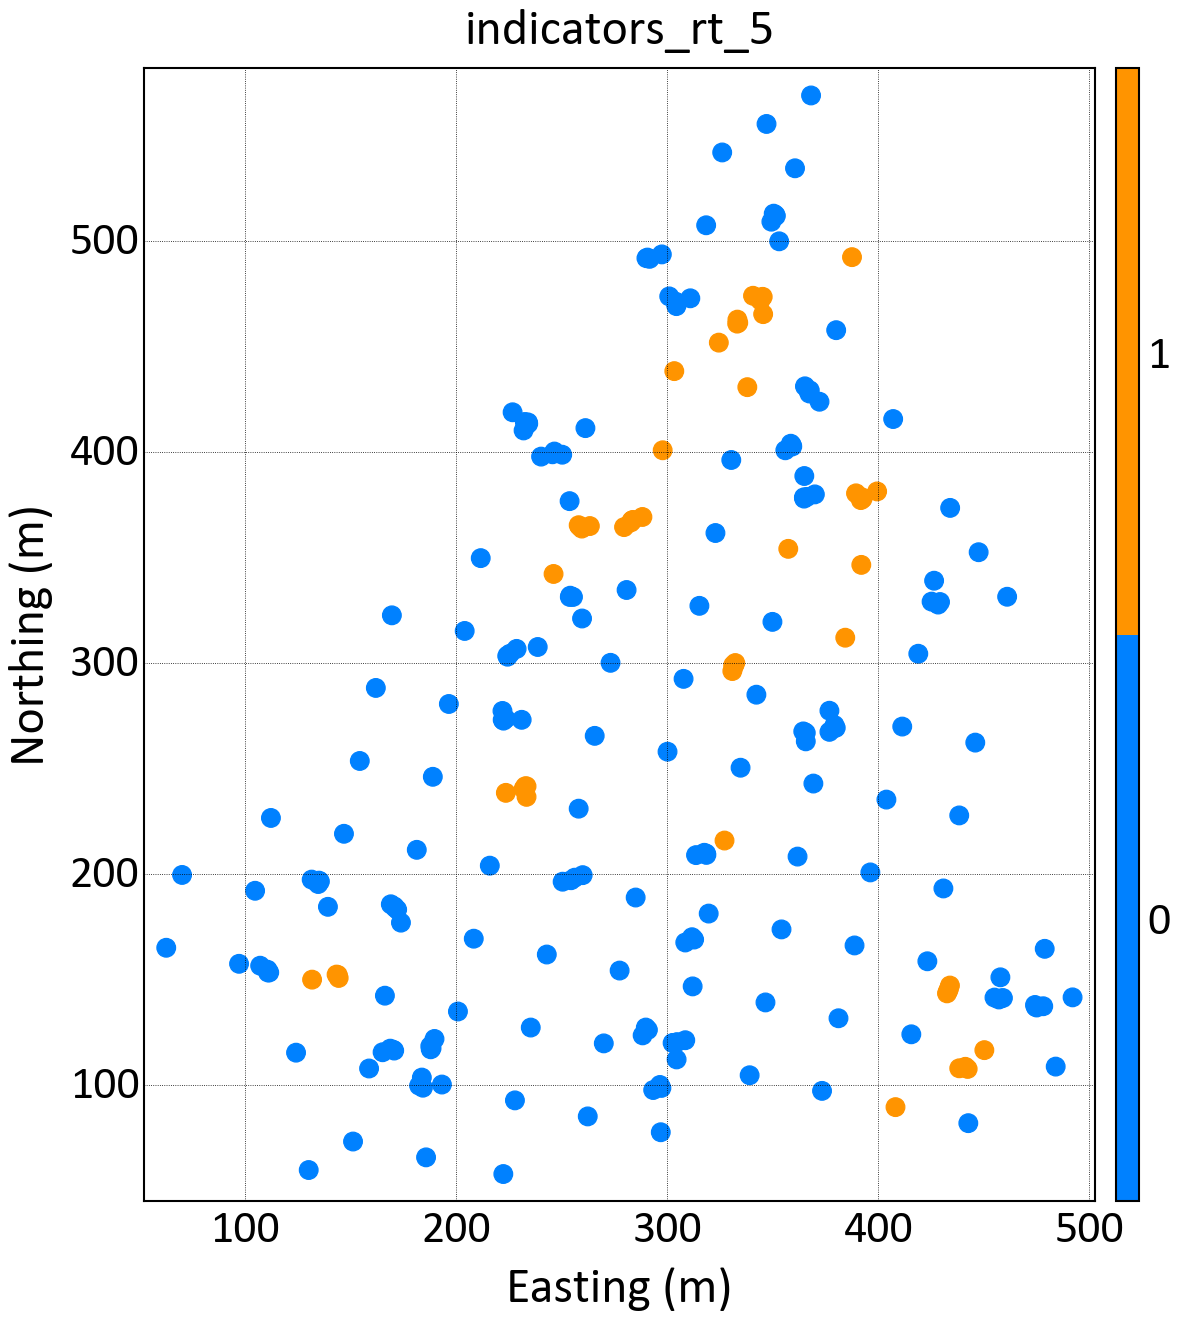
\includegraphics[width=0.6\textwidth]{capitulo_2/imagens/ind5.png}
\end{figure}

O segundo passo é o cálculo das distâncias assinaladas. Para cada ponto amostral, a menor distância euclideana até um outro ponto amostral que pertença a um indicador oposto é computada, e esse valor atribuído àquele ponto, com o sinal negativo caso pertença ao domínio modelado e com o sinal positivo, caso contrário, como ilustrado na \autoref{2d_ex}. 

\begin{figure}[H]
    \centering
	\caption{\label{2d_ex}Ilustração esquemática mostrando o cálculo das distâncias assinaladas.}
	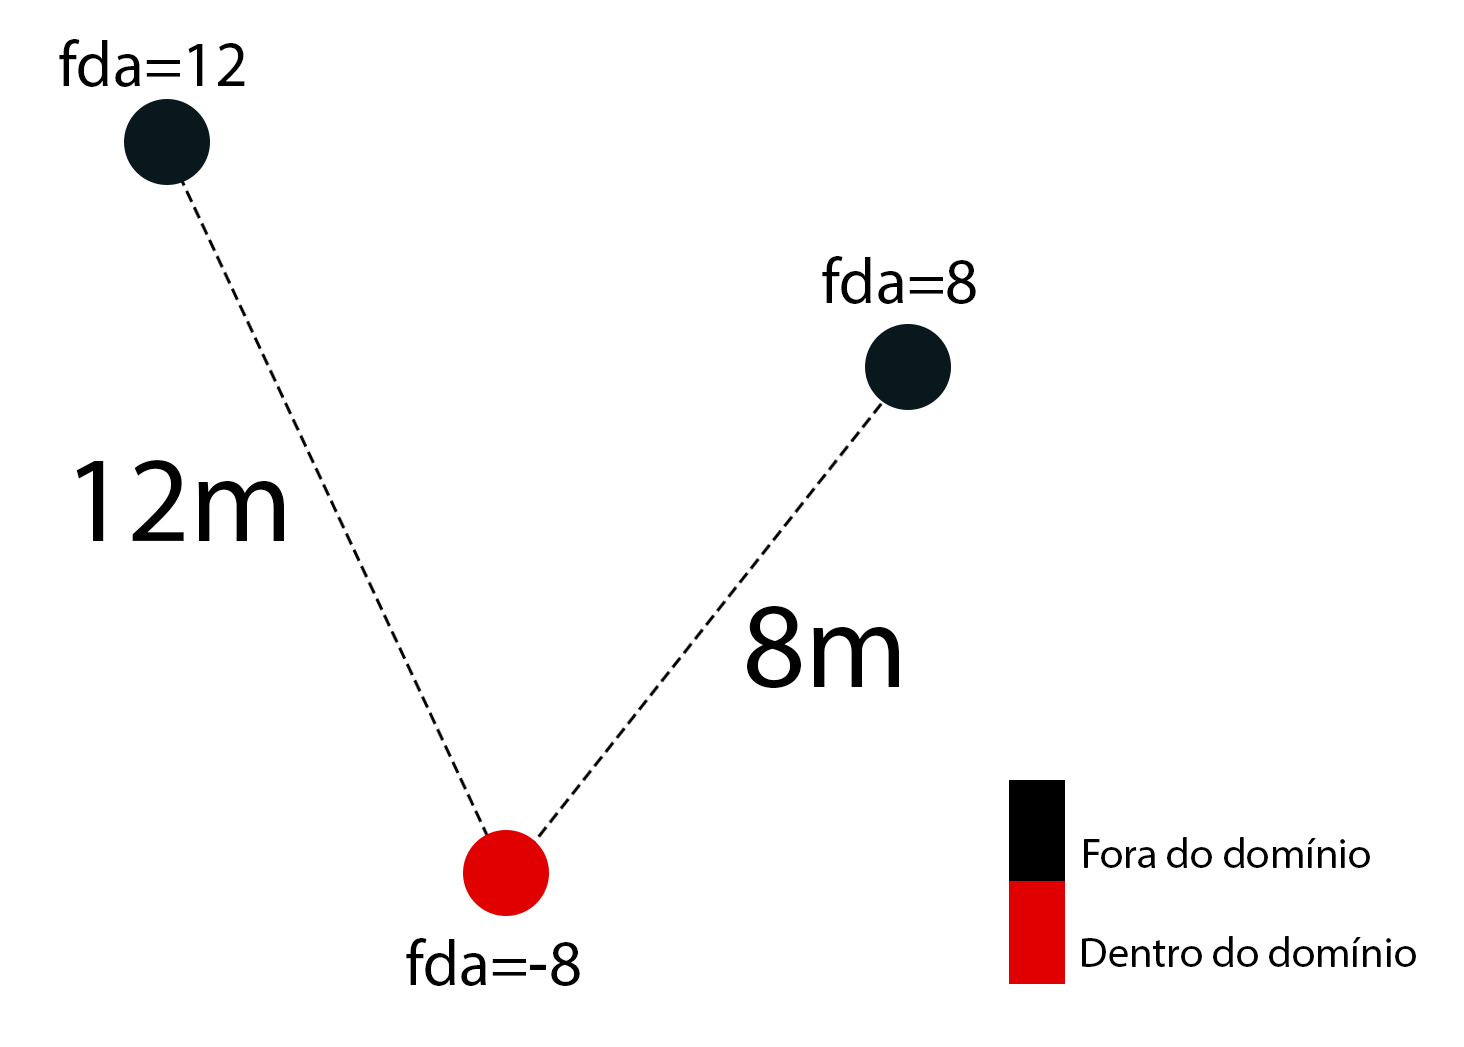
\includegraphics[width=0.6\textwidth]{capitulo_2/imagens/2d_ex.jpg}
\end{figure}

Desse modo, o valor da função distância assinalada $d_k$ para a o domínio $k$ modelado no local $u_\alpha$ é:

\begin{equation}
	d_k(u_\alpha)=\begin{cases}
	-\parallel u_\alpha-u_\beta\parallel,\:\textrm{se $u_\alpha$ pertence ao domínio}\\
	+\parallel u_\alpha-u_\beta\parallel,\:\textrm{se $u_\alpha$ não pertence ao domínio}\end{cases}
    \label{eq_mult_sg}
\end{equation}

O local $u_\beta$ corresponde à amostra mais próxima codificada com um indicador diferente de $u_\alpha$.

A \autoref{sd5} mostra as distâncias assinaladas calculadas para a categoria Quaternary do \textit{Swiss Jura}.

\begin{figure}[H]
	\centering
	\caption{\label{sd5}Mapa de localização das distâncias assinaladas para a categoria Quaternary do \textit{dataset} \textit{Swiss Jura}.}
	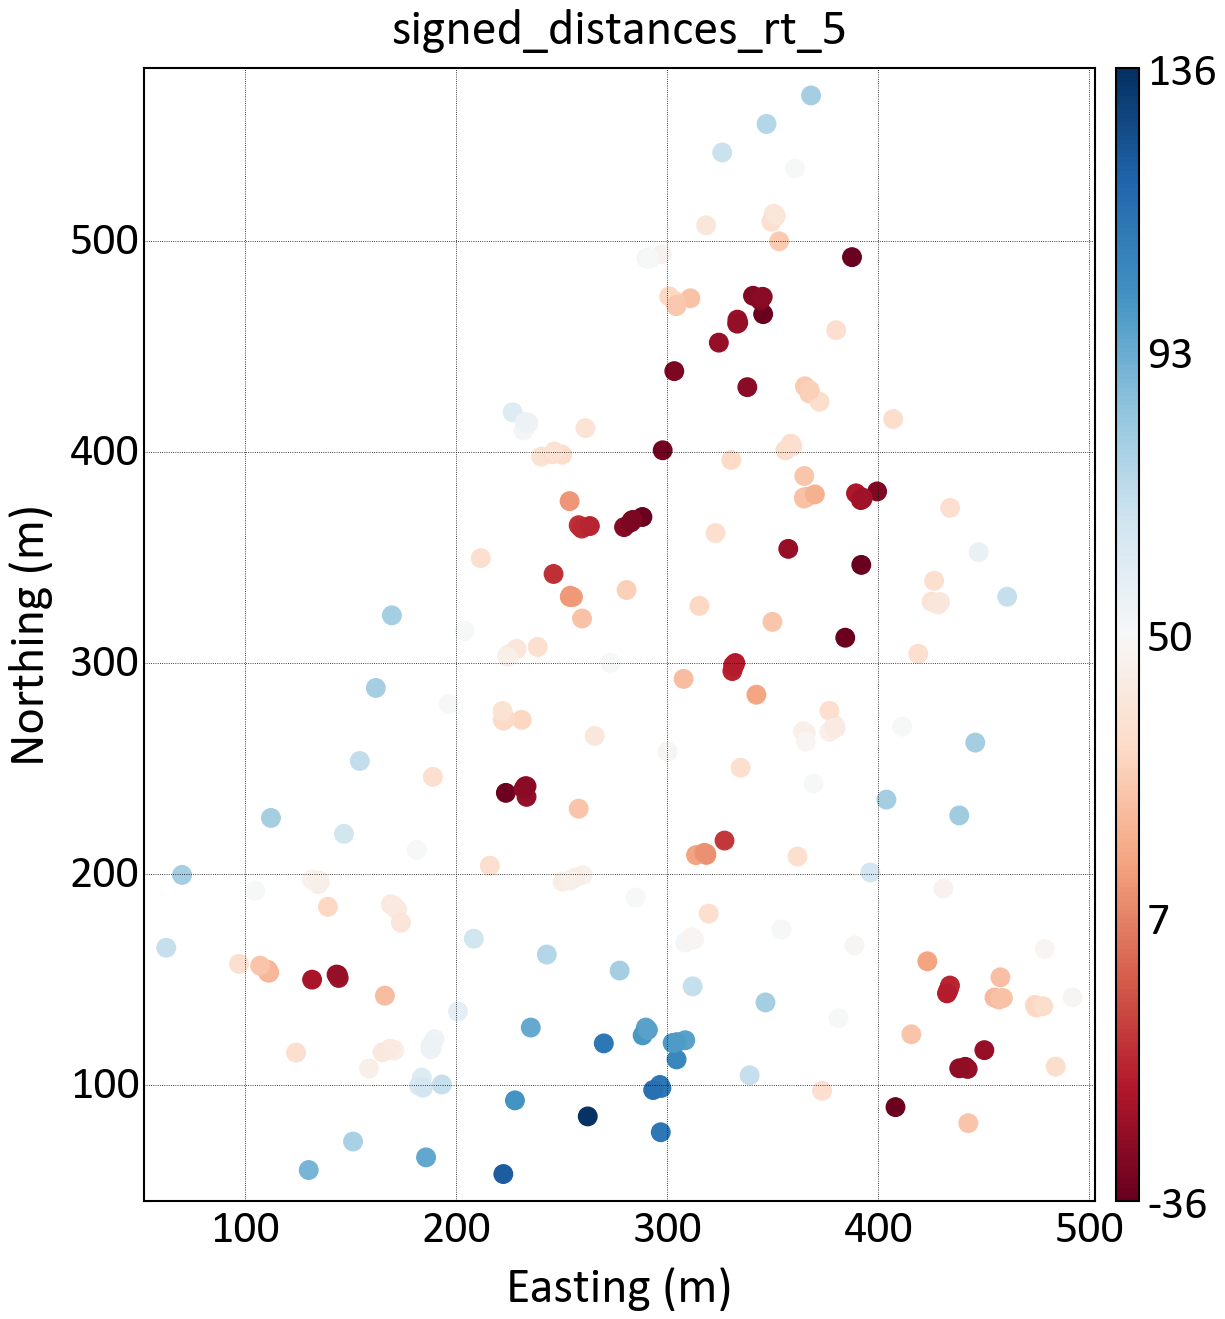
\includegraphics[width=0.6\textwidth]{capitulo_2/imagens/sd5.png}
\end{figure}

Para corpos geológicos que se estendem muito mais em uma direção em relação às demais, como os corpos tabulares por exemplo, as distâncias calculadas podem ser anisotrópicas. Sendo assim, as coordenadas originais $x$, $y$ e $z$ dos dados devem ser rotacionadas e/ou contraídas/dilatadas, a partir da transformação da \autoref{eq_rot_matrix}. Então, as distâncias euclideanas (\autoref{eq_mult_sg}) são calculadas normalmente para as novas coordenadas $x''$, $y''$, $z''$.

\begin{equation}
\resizebox{.9 \textwidth}{!}{%
$
\begin{bmatrix} x'' \\ y'' \\ z'' \end{bmatrix} = \begin{bmatrix} \frac{1}{a_{max}} & 0 & 0 \\ 0 & \frac{1}{a_{min}} & 0 \\ 0 & 0 & \frac{1}{a_{vert}} \end{bmatrix} \\ \begin{bmatrix}\cos\alpha\cos\phi-\sin\alpha\sin\beta\sin\phi & -\sin\alpha\cos\phi-\cos\alpha\sin\beta\sin\phi & \cos\beta\sin\phi \\ \sin\alpha\cos\beta & \cos\alpha\cos\beta & \sin\beta \\ -\cos\alpha\sin\phi-\sin\alpha\sin\beta\cos\phi & \sin\alpha\sin\phi-\cos\alpha\sin\beta\cos\phi & \cos\beta\cos\phi \end{bmatrix} \begin{bmatrix} x \\ y \\ z \end{bmatrix}
$
}
\label{eq_rot_matrix}
\end{equation}

Onde $a_{max}$, $a_{min}$ e $a_{vert}$ são as dimensões dos eixos máximo, médio e mínimo, e $\alpha$, $\beta$ e $\phi$, os ângulos de azimute, mergulho e \textit{rake} que caracterizam os eixos de anisotropia.

\subsubsection{Variografia}

No caso das distâncias assinaladas, obter um modelo de covariância a partir dos variogramas experimentais não é trivial. Distâncias assinaladas não são estacionárias, por isso, o variograma não se estabiliza em um patamar. Além disso, o caráter extremamente contínuo das distâncias torna a identificação analítica das direções principais um processo embaraçoso.

\citeonline{manchuck_deutsch_Geometric} sugerem alternativas para modelagem do variograma das distâncias:

\begin{itemize}
    \item Treinar o variograma usando validação cruzada;
    \item Tentar modelar interativamente os variogramas experimentais;
    \item Calcular e modelar os variogramas para as propriedades de indicadores e transformá-los em um equivalente Gaussiano para as distâncias assinaladas baseado na similidade entre a simulação Gaussiana truncada e a modelagem geológica com funções distância assinaladas. Um campo Gaussiano diferenciável e contínuo é gerado e truncado em um limiar para que a proporção correta de um indicador particular seja o resultado. Entretanto, na prática, o variograma dos indicadores é usado para parametrizar o variograma das distâncias assinaladas de forma direta \cite{martin2017implicitmodeling};
    \item Inferir um modelo de covariância plausível a partir de mapas delineados a mão em \textit{softwares} de iso-contorno.
\end{itemize}

Uma outra alternativa ao cálculo e modelagem de variogramas é o uso de tabelas de covariância proposto por \citeonline{kloechner_cov_table}, esse estudo propõe a substituição da modelagem tradicional dos variogramas por tabelas de covariância, tornando o processo de modelagem geológica completamente automático e livre da subjetividade do geomodelador.

O alcance do variograma, juntamente com a anisotropia, controlam a extensão e forma dos domínios modelados. Os variogramas experimentais das distâncias assinaladas não exibem efeito pepita. Porém, pode ser adicionado arbitrariamente pelo usuário para controlar a interconectividade dos domínios, adicionar ruído ao modelo quando desejável e controlar a extrapolação que pode ser ser excessiva em alguns casos devido à alta continuidade dos modelos Gaussianos.

A \autoref{jura_vargs} mostra o variograma omnidirecional dos indicadores para as categorias do \textit{Swiss Jura}. Os variogramas foram modelados com uma estrutura esférica e efeito pepita zero.

\begin{figure}[H]
    \caption{Variogramas omnidirecionais dos indicadores.} \label{jura_vargs}
     \centering
     \subfloat[][Argovian.]{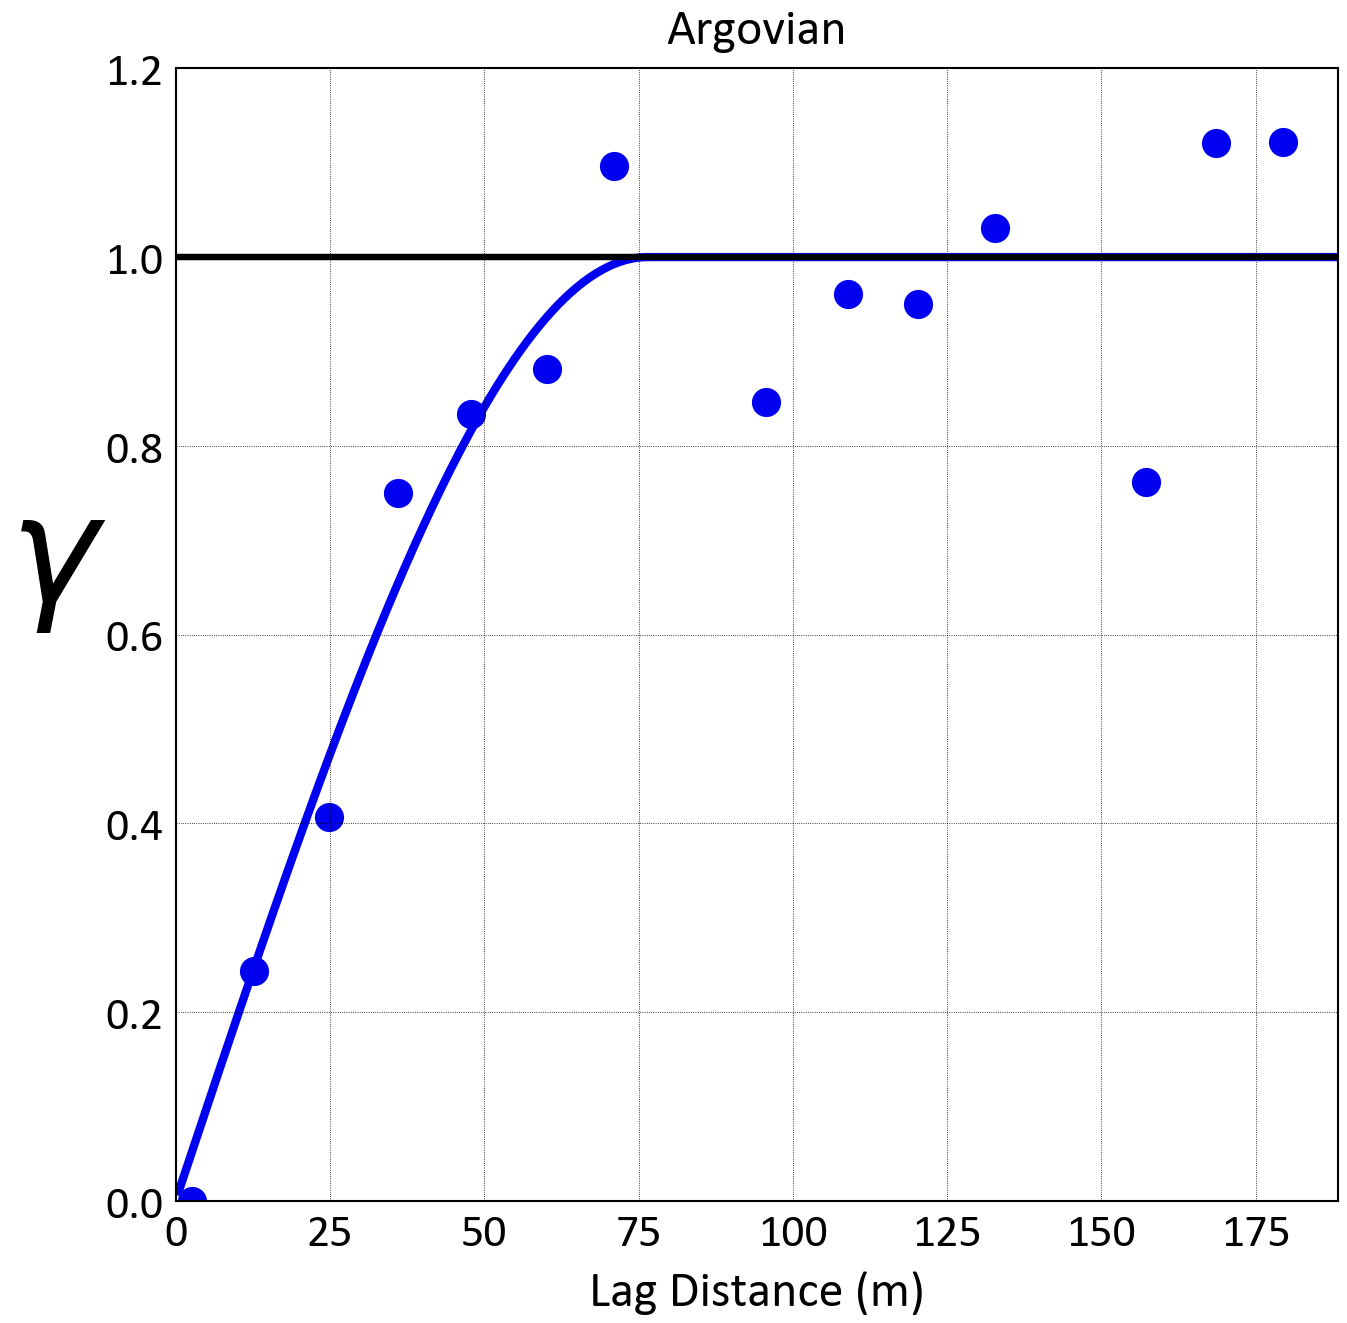
\includegraphics[width=0.45\textwidth]{capitulo_2/imagens/jura_var_1.png}\label{fig:jv1}}
     \hspace{1em}
     \subfloat[][Kimmeridgian.]{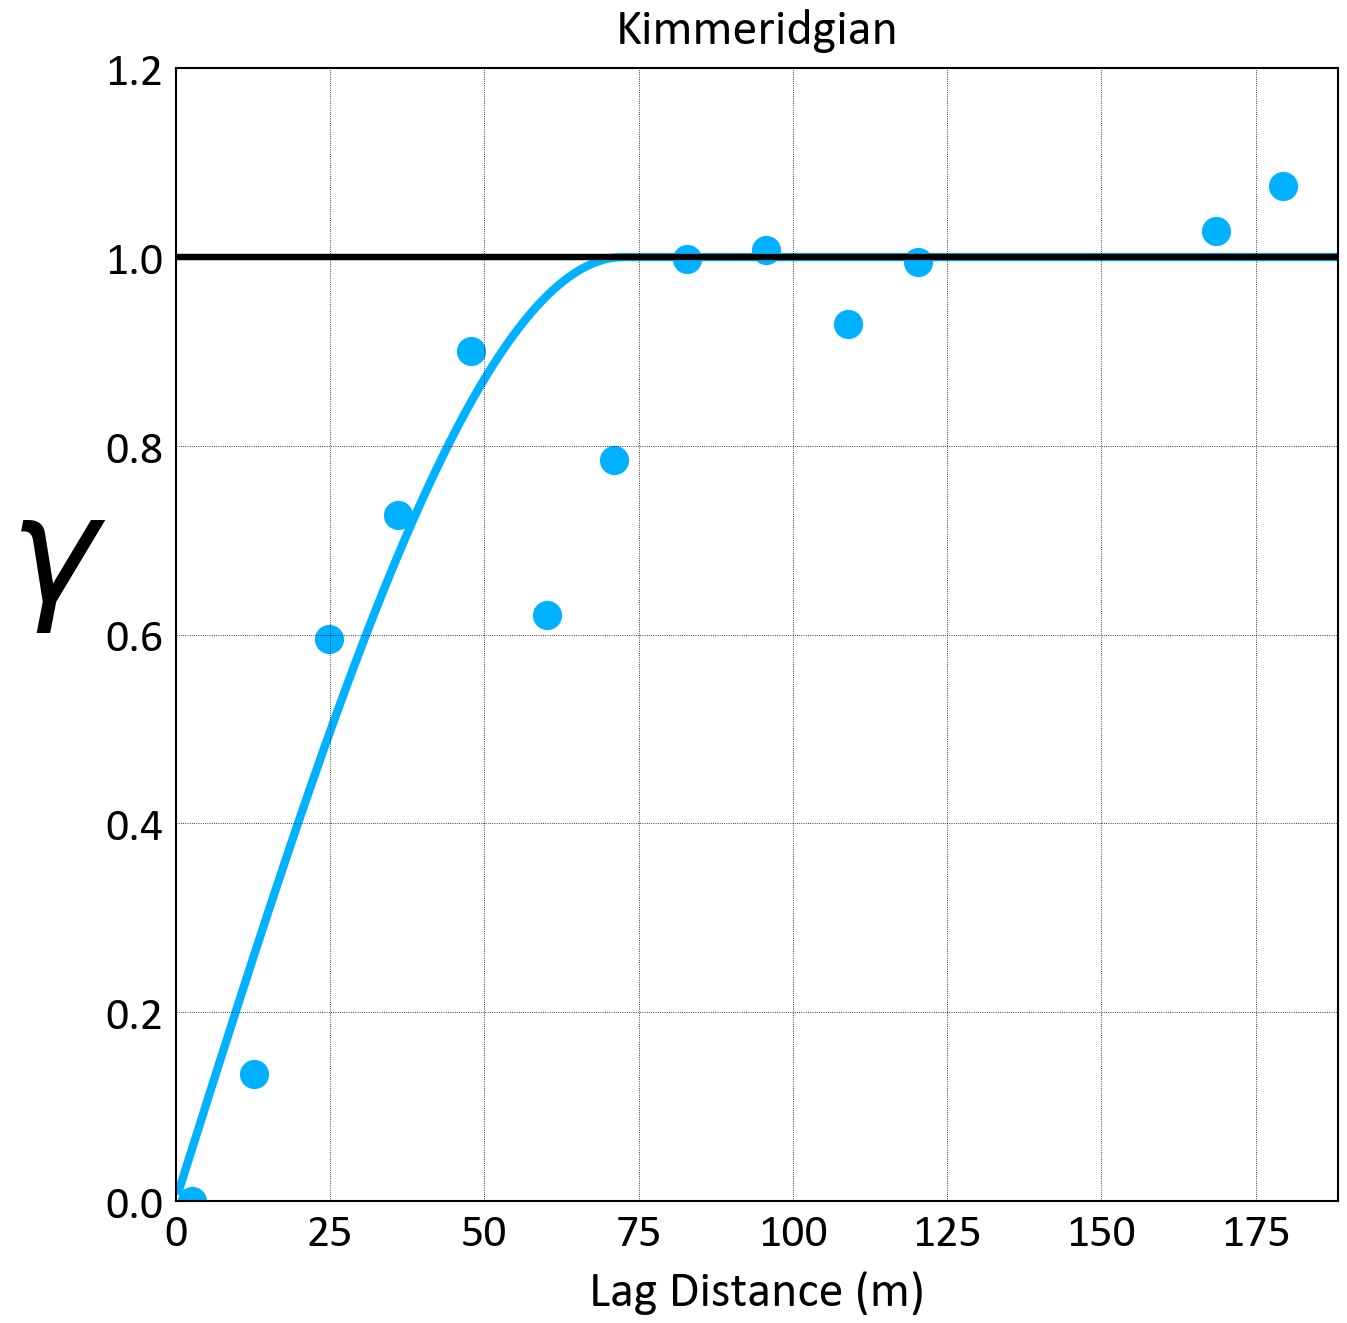
\includegraphics[width=0.45\textwidth]{capitulo_2/imagens/jura_var_2.png}\label{fig:jv2}}\\
    \subfloat[][Sequian.]{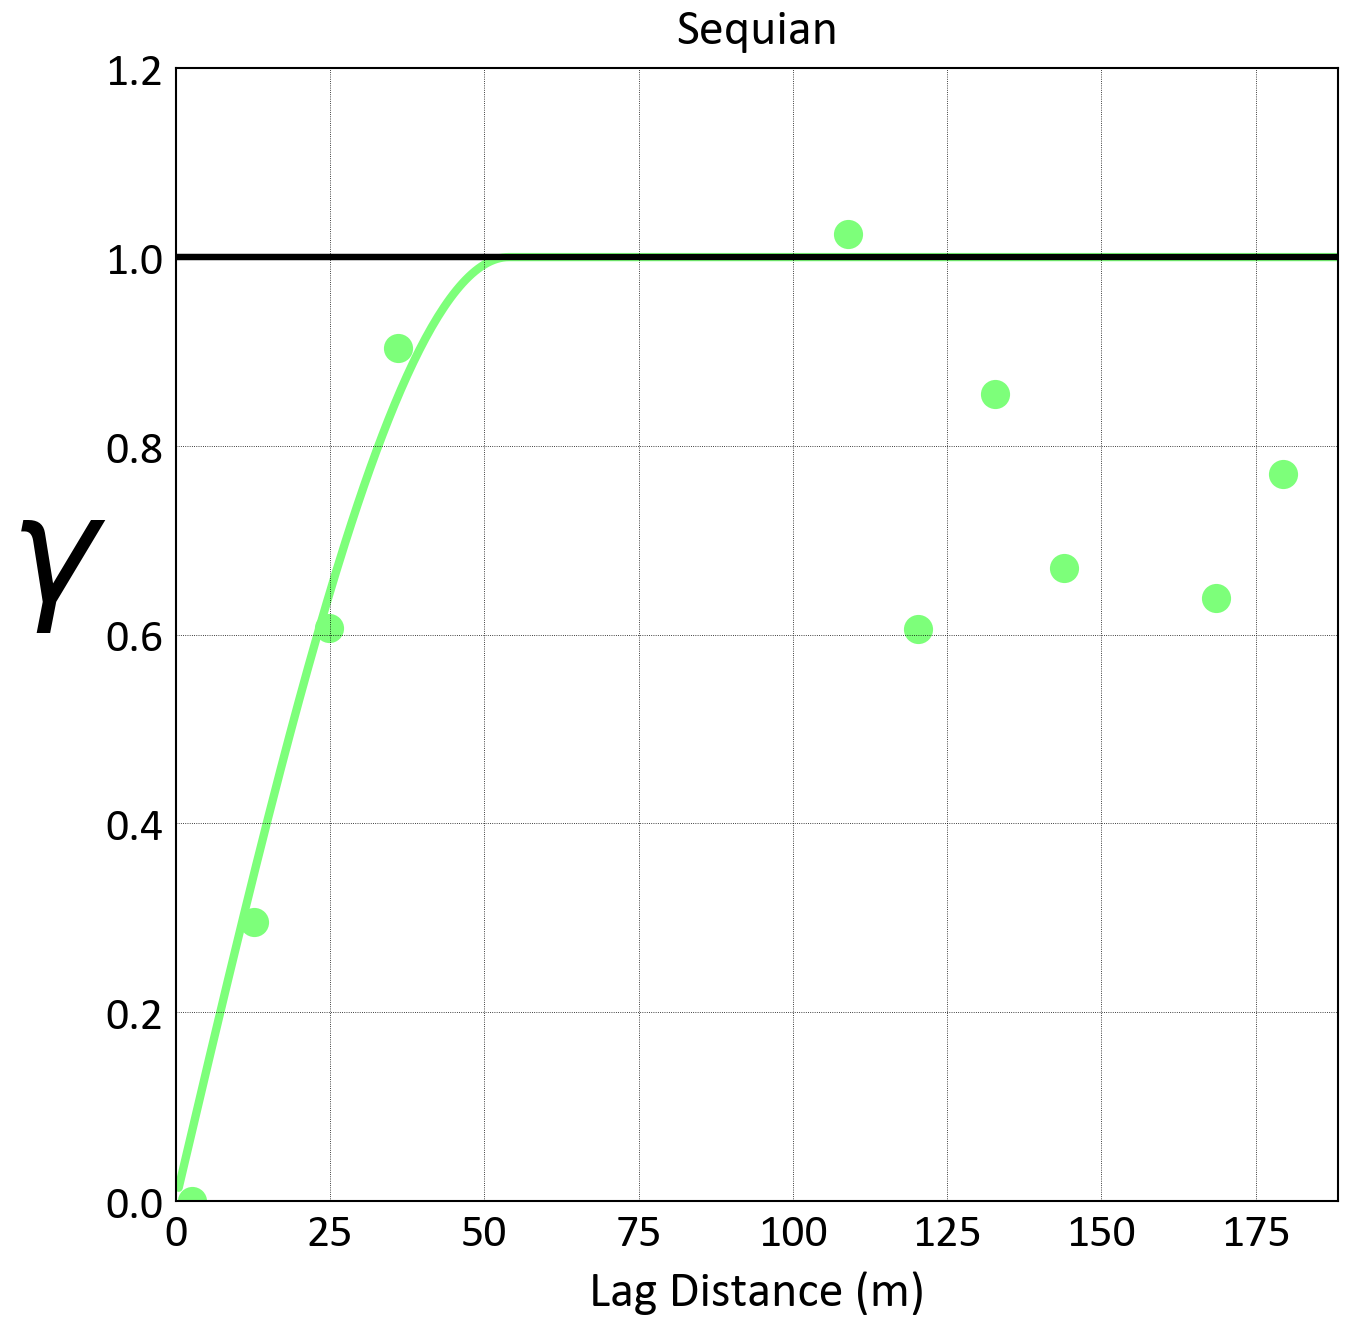
\includegraphics[width=0.45\textwidth]{capitulo_2/imagens/jura_var_3.png}\label{fig:jv3}}
    \hspace{1em}
    \subfloat[][Portland.]{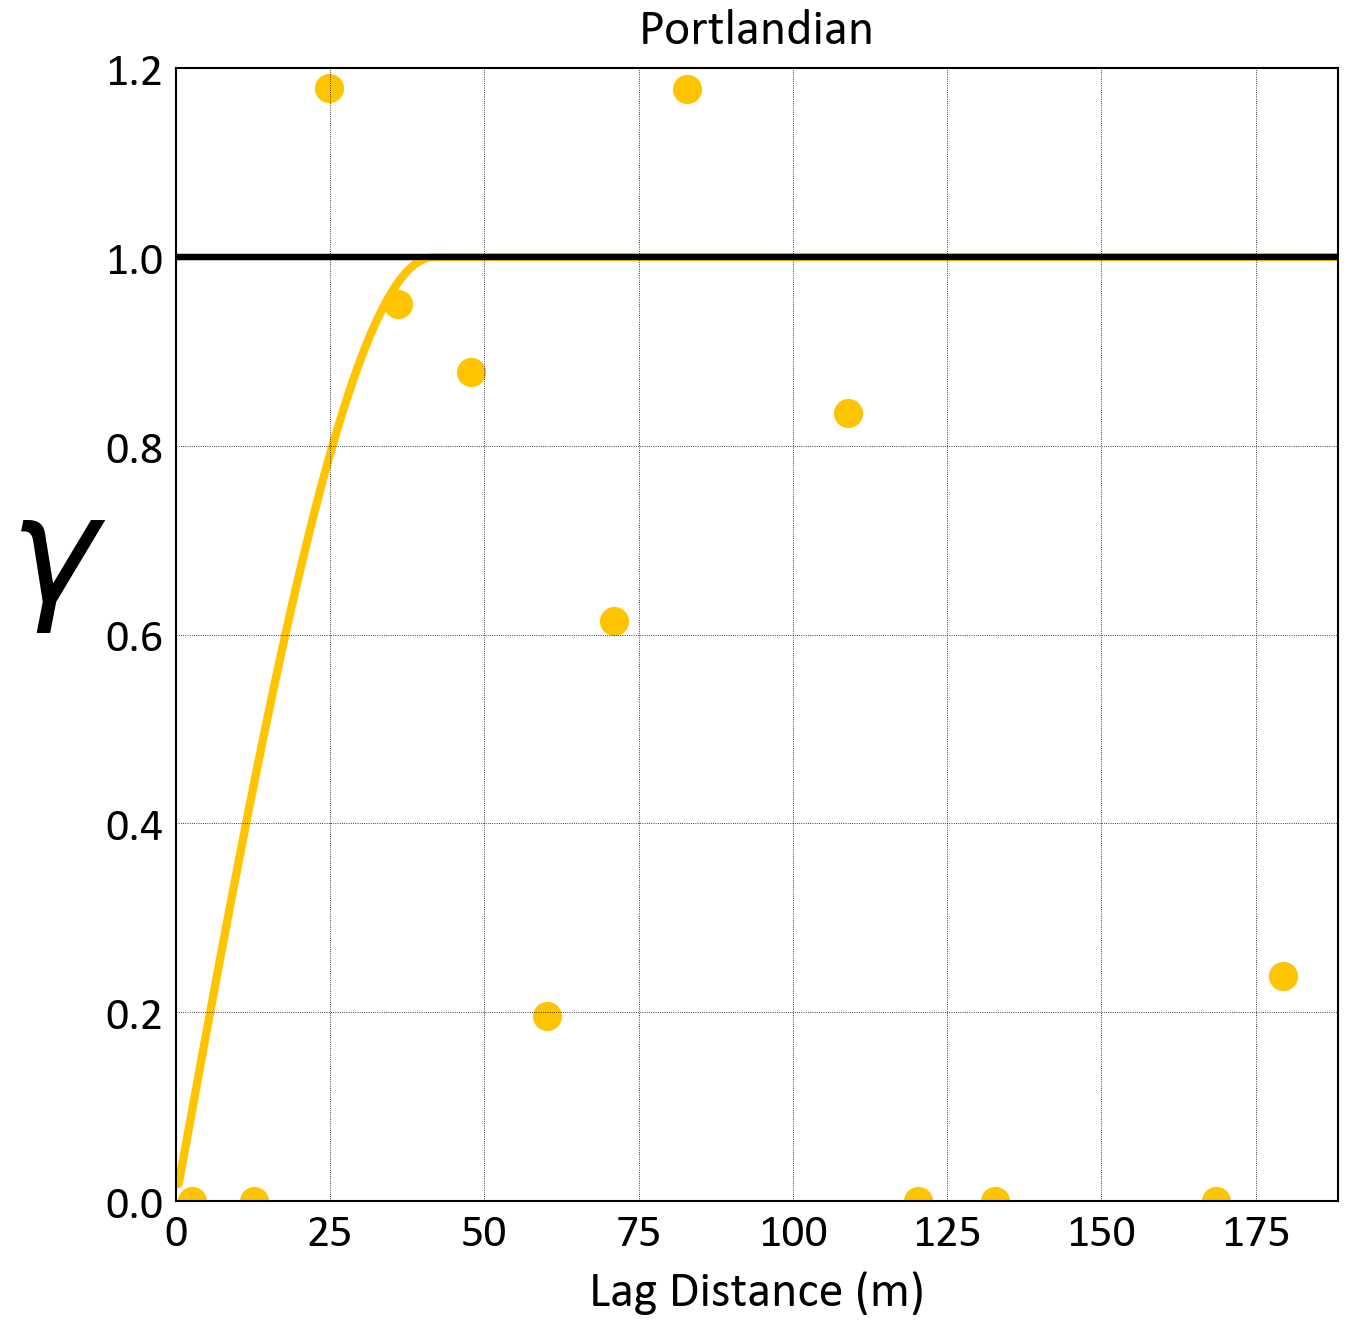
\includegraphics[width=0.45\textwidth]{capitulo_2/imagens/jura_var_4.png}\label{fig:jv4}} \\
    \subfloat[][Quaternary.]{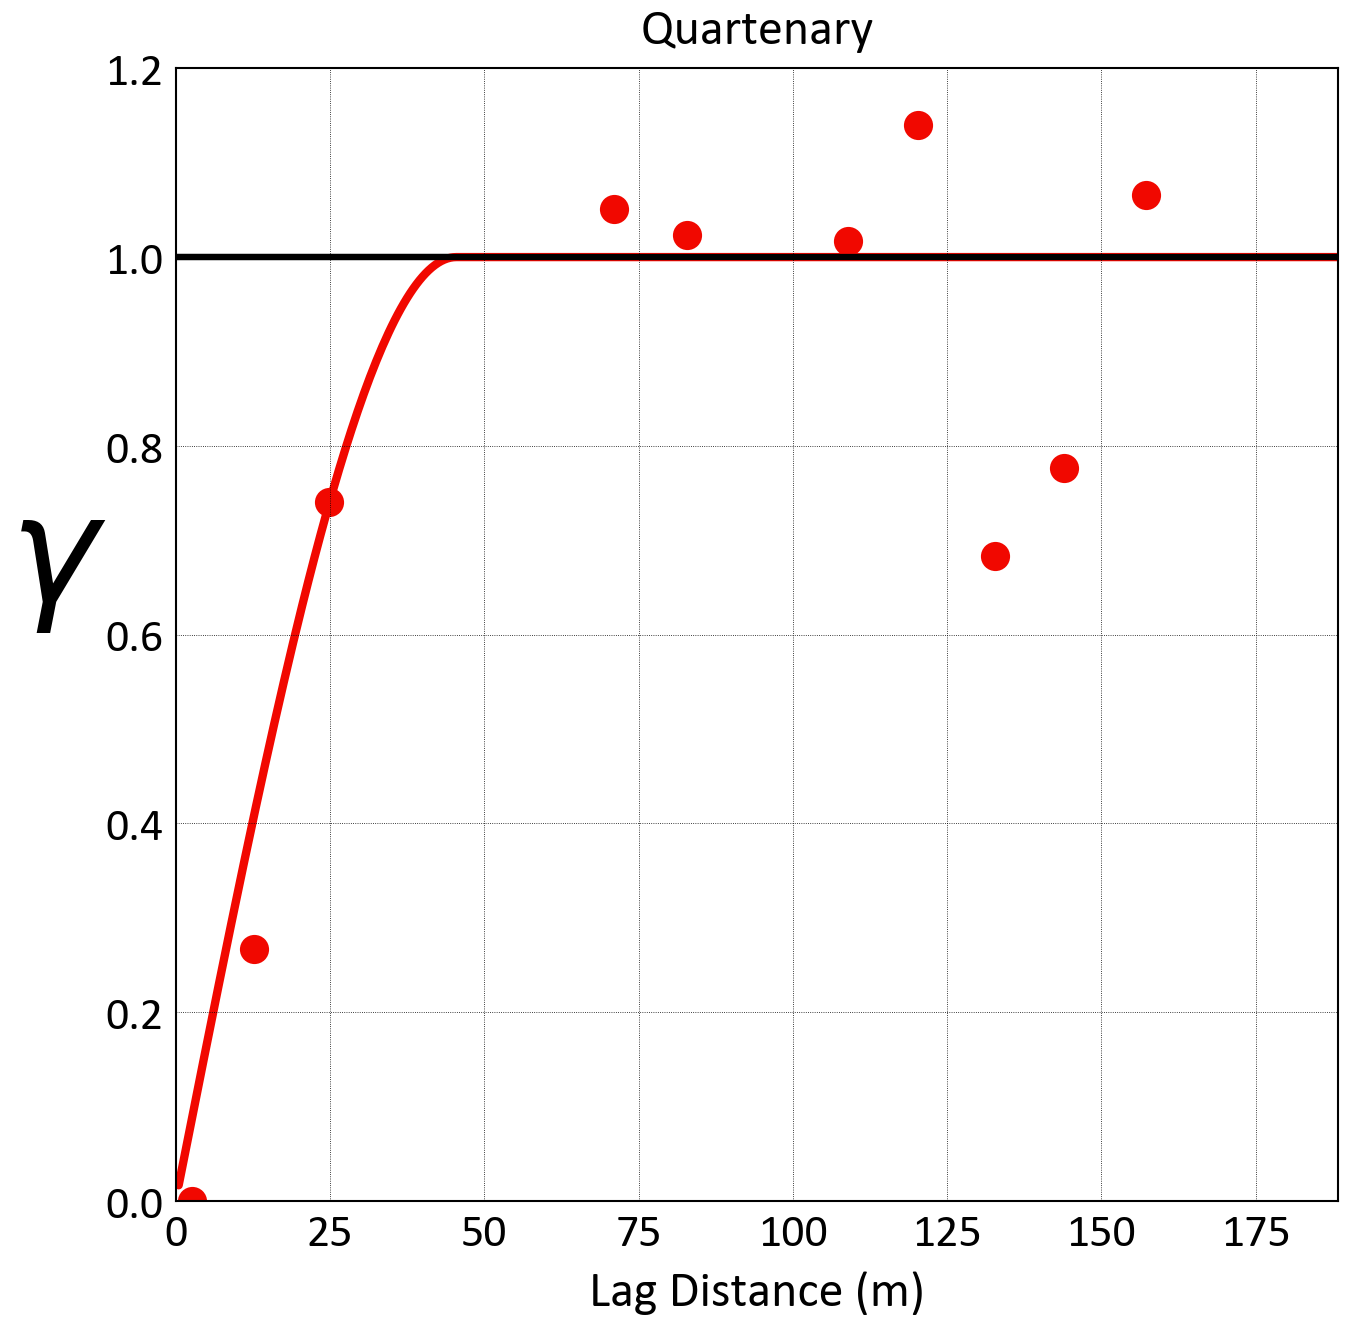
\includegraphics[width=0.45\textwidth]{capitulo_2/imagens/jura_var_5.png}\label{fig:jv5}}
\end{figure}

As equações: \autoref{var_argovian}, \autoref{var_kime}, \autoref{var_sequ}, \autoref{var_port}, \autoref{var_quart} representam os variogramas das cartegorias \textit{Argovian; Kimmeridgian; Sequian;
Portlandian; e Quartenary}, respectivamente.

\begin{equation}
    \label{var_argovian}
    \gamma(h)=1.0Sph_{1} \left[ \frac{OMNI}{76 m} \right]
\end{equation}

\begin{equation}
    \label{var_kime}
    \gamma(h)=1.0Sph_{1} \left[ \frac{OMNI}{72 m} \right]
\end{equation}

\begin{equation}
    \label{var_sequ}
    \gamma(h)=1.0Sph_{1} \left[ \frac{OMNI}{53 m} \right]
\end{equation}

\begin{equation}
    \label{var_port}
    \gamma(h)=1.0Sph_{1} \left[ \frac{OMNI}{41 m} \right]
\end{equation}

\begin{equation}
    \label{var_quart}
    \gamma(h)=1.0Sph_{1} \left[ \frac{OMNI}{45 m} \right]
\end{equation}

\subsubsection{Interpolação}

Uma vez que as distâncias tenham sido calculadas a partir da localização das amostras, o próximo passo é interpolar as propriedades distância assinaladas para o \textit{grid} definido para a modelagem geológica. Embora métodos implícitos não demandem um \textit{grid} - são métodos conhecidos como \textit{gridless} - o objetivo final é preencher o \textit{grid} de estimativas com as categorias correspondentes ou visualizar o modelo através de isosuperfícies. Técnicas de extração de isosuperfícies exigem a função volumétrica definida exaustivamente em um \textit{grid} retilíneo  \cite{martin2017implicitmodeling}.

Para um número constante de amostras, o tempo necessário para interpolação da função volume para todos os nós do \textit{grid} aumenta linearmente com o número de nós. Os parâmetros do \textit{grid} de estimativas, muitas vezes, são determinado por requisitos de engenharia do projeto. Todavia, o \textit{grid} para definição do modelo geológico pode ser diferente do \textit{grid} definido para os modelos numéricos de teores. A consideração mais importante é a capacidade de reproduzir a menor estrutura geológica de interesse.

Considere as seções de um modelo geológico na \autoref{grid_res} gerados em \textit{grids} de diferentes resoluções.

\begin{figure}[H]
	\centering
	\caption{\label{grid_res}Efeito da resolução do \textit{grid} na reprodução de estruturas geológicas.}
	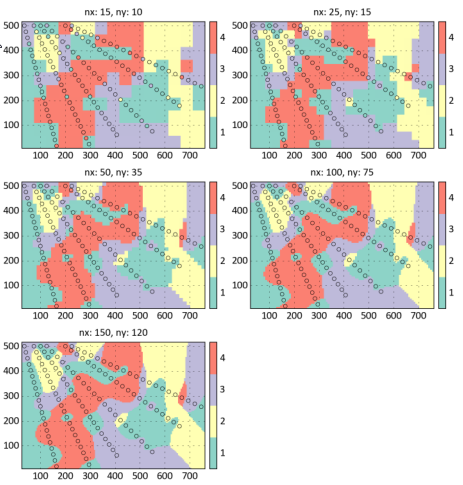
\includegraphics[width=0.6\textwidth]{capitulo_2/imagens/grid_res.png}
	\legend{Fonte: \citeonline{martin2017implicitmodeling}}
\end{figure}

A resolução adequada para esse modelo é entre (nx, ny) = (50, 35) e (nx, ny) = (100, 75). Para os dois primeiros \textit{grids} mais grosseiros há classificação errônea dos nós colocados com amostras, além de (nx, ny) = (100, 75) há pouco benefício na reprodução das estruturas levando em consideração o aumento do tempo de interpolação.

É preciso encontrar um balanço entre resolução e tempo de interpolação. A resolução do \textit{grid} pode ser aumentada a medida que o projeto avança e mais informação é adquirida \cite{martin2017implicitmodeling}.

Qualquer método de interpolação pode ser utilizado, mesmo os métodos do inverso da distância produzem resultados realistas. A krigagem e as funções de bases radiais permitem incorporar informação adicional através dos modelos de covariância parametrizados a partir das amostras.

\citeonline{hosseini_deutsch_iqd} utilizaram inverso da distância, \citeonline{silvaenhancedgeomodeling} utilizou krigagem  global, \citeonline{rolo_dissertacao} utilizou krigagem ordinária, \citeonline{silva_dual} aplicaram krigagem dual. \citeonline{boisvert_geomodeling} gerou modelos implícitos através de distâncias assinaladas com anisotropia variável local (\textit{Locally varying anisotropy kriging - LVA}) e \citeonline{cowan2002rapid} propuseram a utilização de interpoladores baseados em funções de bases radias (\textit{radial basis functions - RBF}), \citeonline{manchuck_MLS} ainda propuseram a utilização de mínimos quadrados móveis para incorporar interpretação manual em seções e avaliar incerteza. A escolha do interpolador deve ser baseada em suas propriedades, na informação exigida para parametrizá-lo (o variograma, por exemplo) e nas sua capacidade de se ajustar a formas geológicas.

Especialmente para as funções distância assinaladas, existe um problema adicional relacionado à estacionariedade de primeira e segunda ordem. Existe uma forte tendência (\textit{trend}) que restringe os estimadores baseados em krigagem para que a estacionariedade seja mantida. Além disso, formas geológicas são curvilíneas e não são bem descritas por funções de covariância "tradicionais" onde a distância euclideana entre os pares de pontos são medidas em linha reta. Por esses motivos muitos autores preferem as funções de bases radiais já que ela não se baseia em estacionariedade de primeira ordem e honram localmente formas geológicas sem a necessidade de parametrização especial \cite{martin2017implicitmodeling}.

Independente do método de interpolação, os modelos gerados devem ser livres de artefatos para que os artefatos do modelo implícito não sejam transferidos para os modelos geológicos. Por esse motivo, interpoladores globais devem ser usados por utilizarem todas as amostras em cada estimativa, já para os métodos baseados em inverso da distância e krigagem (não global) os parâmetros de busca são uma escolha crítica \cite{martin2017implicitmodeling}. Em contrapartida, métodos globais possuem limitações em bancos de dados volumosos por dependerem de muito processamento e memória RAM.

A \autoref{interpsd5} mostra as distâncias assinaladas para a categoria Quaternary do \textit{Swiss Jura} interpolada por krigagem dual (\autoref{dksection}) em um grid 3x3 metros. O variograma dos indicadores da Figura \autoref{fig:jv5} foi usado para para parametrizar o variograma Gaussiano - mesmas estruturas, mesmos ranges, mesmas relações e ângulos de anisotropia.

\begin{figure}[H]
	\centering
	\caption{\label{interpsd5}Categoria Quaternary do \textit{Swiss Jura} interpolada por krigagem dual em um grid 3x3 metros.}
	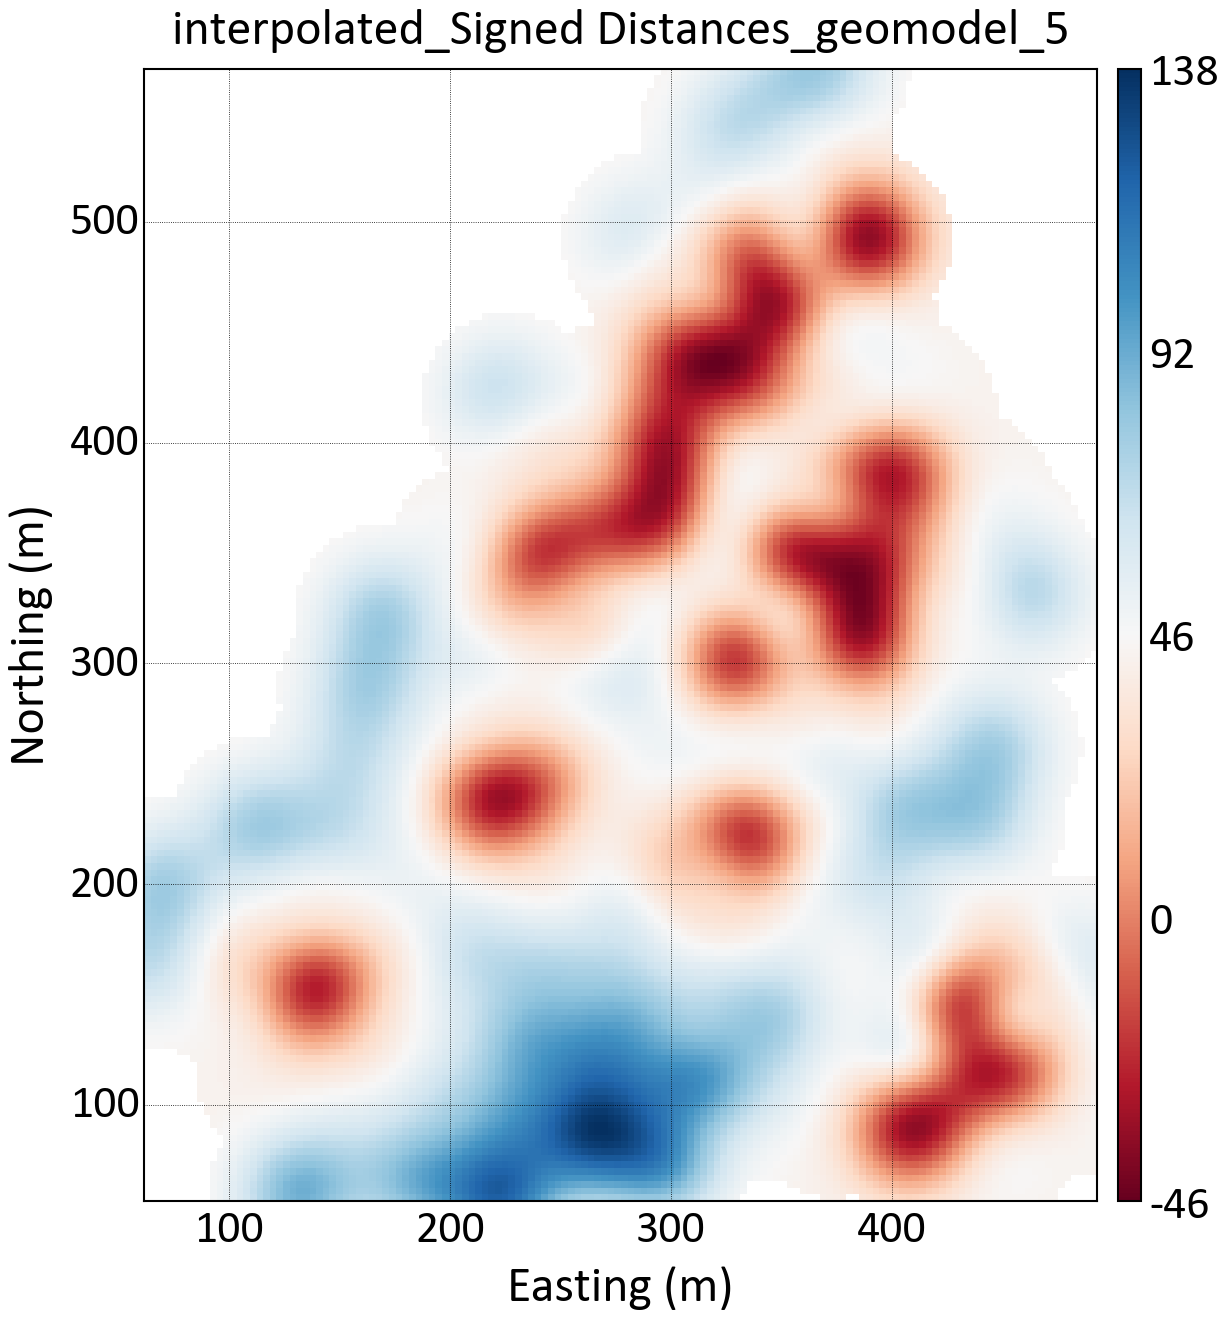
\includegraphics[width=0.6\textwidth]{capitulo_2/imagens/int_sd_5.png}
\end{figure}

Os principais interpoladores globais são listados a seguir.

\subsubsubsection{Krigagem global}

A krigagem global \cite{neufeldglobalkriging} não produz nenhum artefato relacionado à estratégia de busca, porque não há estratégia de busca. O algoritmo lê todos os dados e usa todos os valores dos dados para estimar cada local não amostrado. Um benefício adicional da krigagem global é a redução do tempo de CPU para o cálculo das estimativas já que não é necessário buscar amostras no espaço e a matriz de covariâncias entre as amostras é calculada e invertida uma única vez. O valor estimado da função distância assinalada para um local não amostrado é dado pela \autoref{estimador_k}:

\begin{equation}
\label{estimador_k}
d^*(u)=\sum_{i=1}^{n} \lambda_i(u) d(u_i)
\end{equation}

Onde: $d^*$ é a distância estimada no local não amostrado $u$, $\lambda_i(u)$ é o peso dado para a distância assinalada $d$ observada no local $u_i$.

Os pesos podem ser calculados resolvendo as equações de krigagem. Neste caso, as equações de krigagem ordinária:

\begin{equation}
    \label{global_k}
    \begin{bmatrix} 
    C_{11}&\dots&C_{1n}&1\\
    \vdots&\ddots&\vdots&1\\
    C_{n1}&\dots&C_{nn}&1\\ 
    1&1&1&0
    \end{bmatrix}
    \begin{bmatrix} 
    \lambda_{1}\\
    \vdots\\
    \lambda_{n}\\ 
    \mu
    \end{bmatrix}
    =
    \begin{bmatrix} 
    C_{10}\\
    \vdots\\
    C_{n0}\\ 
    1
    \end{bmatrix}
\end{equation}

Onde $C_{ij}$ é a covariância entre as amostras $i$ e $j$, $C_{i0}$ é a covariância entre a amostra $i$ e o local a ser estimado, $n$ é o número de amostras no dataset e $\mu$ é o operador lagrangeano necessário para a krigagem ordinária \cite{isaaks1989applied}. A condição de não enviesamento é $\sum_{i=1}^{n} \lambda_i=1$.

\subsubsubsection{Krigagem dual} \label{dksection}

A krigagem dual \cite{royer1984dual} é uma representação alternativa da krigagem na qual as estimativas são expressas como uma combinação linear das covariâncias ao invés das amostras. Dessa forma, o estimador da \autoref{dk} torna-se:

\begin{equation}
\label{dk}
d^*(u)=\sum_{i=1}^{n} \omega_i C(u-u_i) + m^*_{OK} \\
\end{equation}

Onde $\omega_i$ é o peso dual associado à covariância $C(u-u_i)$ e $m^*_{OK}$ é uma estimativa da tendência (\textit{trend}). A condição de não enviesamento é $\sum_{i=1}^{n} d_i=0$

Ao contrário da krigagem simples e ordinária o sistema de equações não resulta da minimização da variância do erro, mas sim da propriedade de exatidão do estimador de krigagem.

Os pesos são calculados resolvendo a \autoref{dual_k}:

\begin{equation}
    \label{dual_k}
    \begin{bmatrix} 
    C_{11}&\dots&C_{1n}&1\\
    \vdots&\ddots&\vdots&1\\
    C_{n1}&\dots&C_{nn}&1\\ 
    1&1&1&0
    \end{bmatrix}
    \begin{bmatrix} 
    \omega_{1}\\
    \vdots\\
    \omega_{n}\\ 
    m^*_{OK}
    \end{bmatrix}
    =
    \begin{bmatrix} 
    d_{1}\\
    \vdots\\
    d_{n}\\ 
    0
    \end{bmatrix}
\end{equation}

Onde $d_{n}$ é o valor da amostra da distância assinalada n. $m^*_{OK}$ e $\omega_i$ precisam ser calculados apenas uma única vez e usados para todas as estimativas.

A krigagem dual não necessariamente deve ser global, todavia, sem nenhuma adaptação, seus benefícios só podem ser capitalizados se uma vizinhança global for usada \cite{aunon2000dual}.

\subsubsubsection{Funções de bases radiais (RBF)}

A interpolação com funções de bases radiais \cite{fasshauer2007meshfree} é uma técnica global semelhante à krigagem dual. As RBFs são baseadas no posicionamento de um \textit{kernel} radial em cada ponto amostral. A superfície interpolada é uma combinação linear desses \textit{kernels}. O \textit{kernel} é análogo ao variograma da krigagem. O estimador é descrito pela \autoref{estimador_r}:

\begin{equation}
\label{estimador_r}
d^*(u)=\sum_{i=1}^{n} \lambda_i \theta(u - u_i)
\end{equation}

Onde $\theta$ é o \textit{kernel}, que pode ser parametrizado a partir do variograma dos indicadores para uma determinada categoria, e $\lambda_i$ são os pesos calculados a partir da solução da \autoref{rbf_sist}:

\begin{equation}
    \label{rbf_sist}
    \begin{bmatrix} 
    \theta_{11}&\dots&\theta_{1n}\\
    \vdots&\ddots&\vdots\\
    \theta_{n1}&\dots&\theta_{nn}\\ 
    \end{bmatrix}
    \begin{bmatrix} 
    \lambda_{1}\\
    \vdots\\
    \lambda_{n}\\ 
    \end{bmatrix}
    =
    \begin{bmatrix} 
    d_{1}\\
    \vdots\\
    d_{n}\\ 
    \end{bmatrix}
\end{equation}

$\theta_{ij}$ é o valor do \textit{kernel} entre as amostras $i$ e $j$.

\citeonline{fasshauer2007meshfree} advoga que o \textit{kernel} pode ser parametrizado pela distância que representa a maior esfera que pode ser colocada entre amostras no domínio. Para modelagem geológica, essa técnica tende a super estimar o suporte em relação à parametrização pelo variograma calculado a partir das amostras \cite{martin2017implicitmodeling}.

\subsubsection{Visualização do modelo geológico}

Como as funções distância são negativas no interior do domínio e positivas no exterior, um bom palpite inicial para a interface que separa os domínios no espaço, seria a linha (em duas dimensões) ou superfície (em três dimensões) que corresponda ao valor zero da função distância assinalada \cite{wildedeutschcalibrate}. Dessa forma, blocos em que a distância estimada tem valor negativo, são classificados como pertencentes ao domínio. Blocos em que a distância estimada tem valor positivo, classificados como não pertencentes ao domínio de acordo com a \autoref{classifier}:

\begin{equation}
	i^*(u)=\begin{cases}
	1,\:\textrm{se}\:d^*(u)\leq0\\
	0,\:\textrm{caso contrário}\end{cases}
    \label{classifier}
\end{equation}

A \autoref{quartenary_model} mostra o modelo geológico para a categoria Quaternary do \textit{Swiss Jura}. 

\begin{figure}[H]
	\centering
	\caption{\label{quartenary_model}Modelo geológico para a categoria Quaternary do \textit{Swiss Jura}.}
	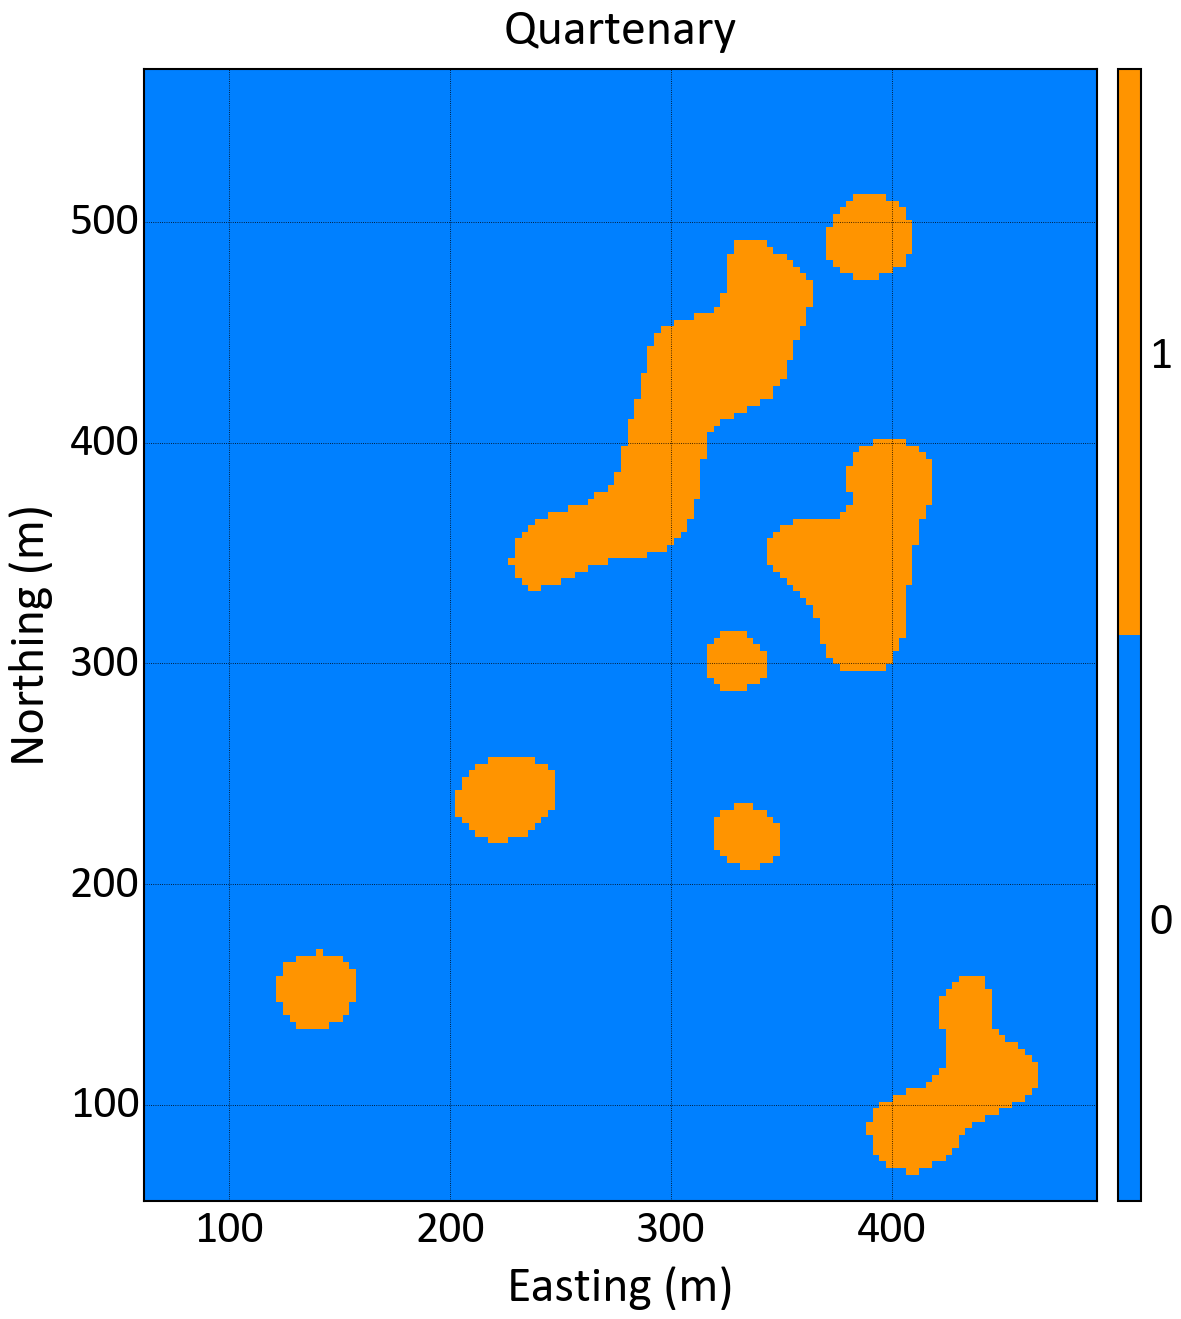
\includegraphics[width=0.6\textwidth]{capitulo_2/imagens/geomodel_quaternary.png}
\end{figure}

A \autoref{one_alt} mostra as coordenadas das distâncias assinaladas estimadas nos eixos x e y e o valor da distância assinalada no eixo z. O plano em cinza corta as distâncias assinaladas na isolinha zero. 

\begin{figure}[H]
	\centering
	\caption{\label{one_alt}Uma outra forma de visualizar a modelagem geológica implícita.}
	\subfloat[][Vista 1.]{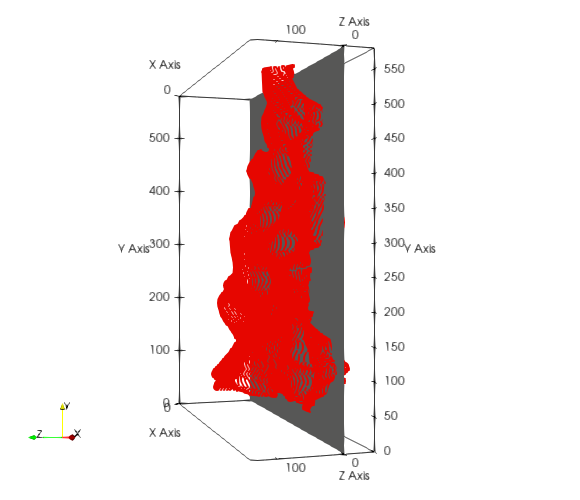
\includegraphics[width=.3\textwidth]{capitulo_2/imagens/one1.png}\label{<figure1>}}
	\hspace{1em}
	\subfloat[][Vista 2.]{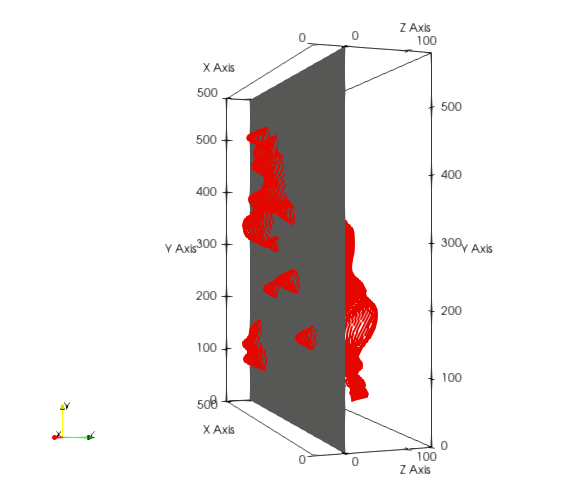
\includegraphics[width=.3\textwidth]{capitulo_2/imagens/one2.png}\label{<figure2>}}
	\hspace{1em}
	\subfloat[][Vista 3.]{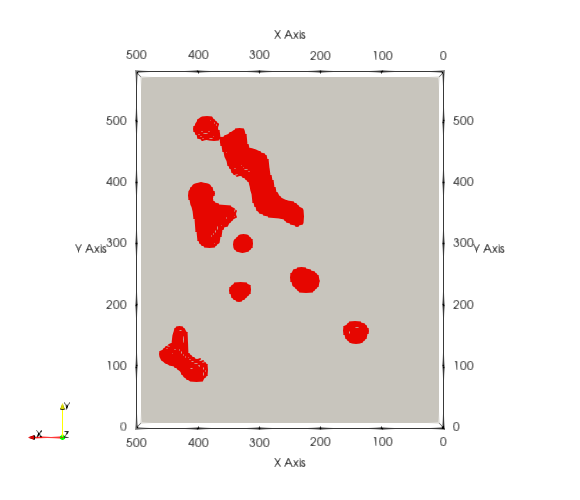
\includegraphics[width=.3\textwidth]{capitulo_2/imagens/one3.png}\label{<figure3>}}
\end{figure}

Em três dimensões um algoritmo de extração de isosuperfícies pode ser aplicado ao modelo implícito para extrair a isosuperfície zero que pode ser posteriormente visualizada como mostrado na \autoref{implicit_3d_ex}. Esse método cria superfícies suaves já que não são delimitadas pelos blocos do \textit{grid} como na \autoref{quartenary_model}. 

\begin{figure}[H]
    \caption{Exemplo mostrando a extração da isosuperfície zero e visualização em três dimensões.} \label{implicit_3d_ex}
     \centering
     \subfloat[][Modelo implícito interpolado por RBF para a categoria sendo modelada.]{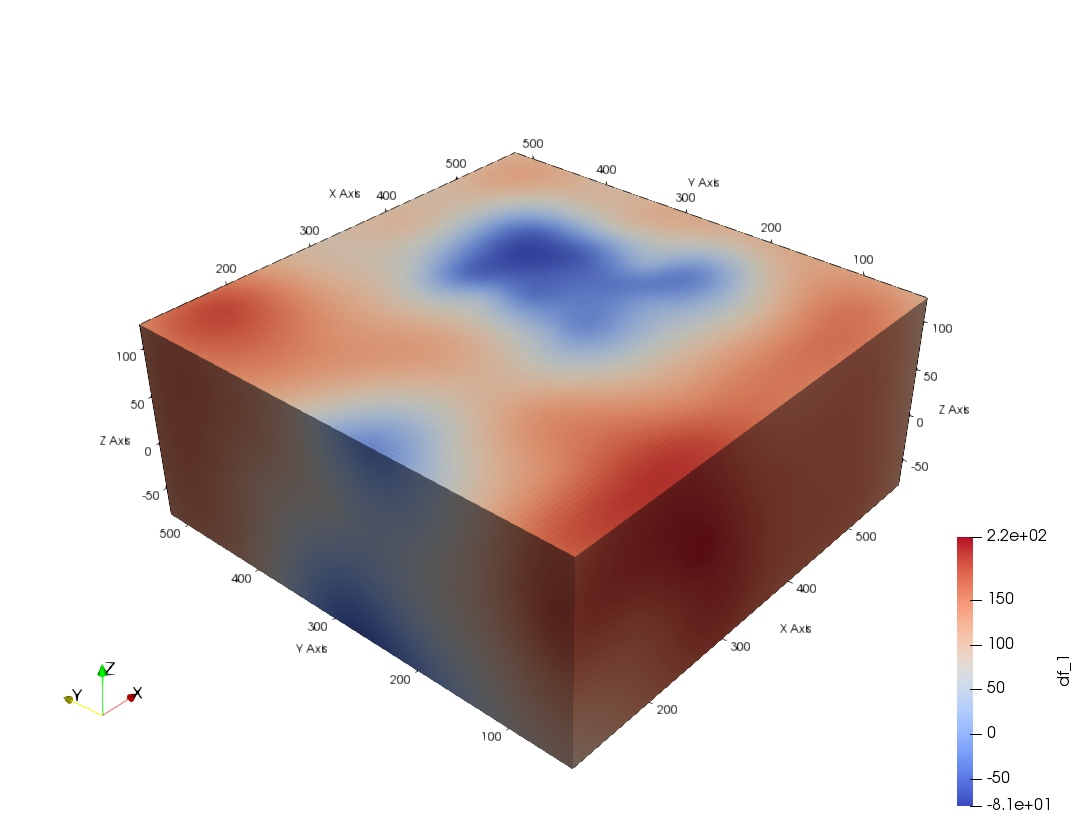
\includegraphics[width=.4\textwidth]{capitulo_2/imagens/rbf.jpeg}\label{fig:c2}}
     \hspace{1em}
     \subfloat[][Isosuperfície zero extraída a partir do modelo implícito.]{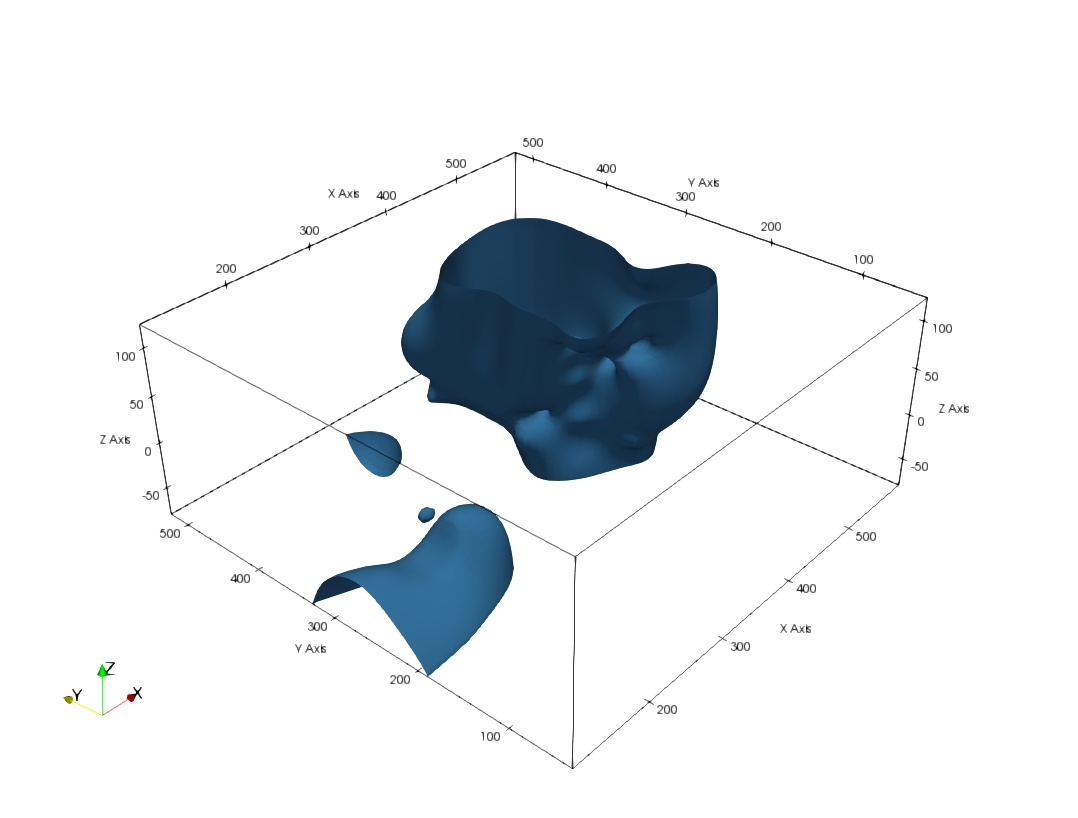
\includegraphics[width=.45\textwidth]{capitulo_2/imagens/isorbf.jpeg}\label{fig:c3}}
\end{figure}

Na presença de múltiplos domínios, as isosuperfícies ou isolinhas, devem ser extraídas uma a uma, e algum tipo de regra hierárquica baseada na idade de cada litologia deve ser aplicada para a criação dos modelos multi-categóricos.

\subsubsection{Adaptação para múltiplas categorias}

\citeonline{silvaanddeutschccgmodeling} propuseram, uma adaptação para o método com o objetivo de modelar múltiplos domínios geológicos simultaneamente, de forma similar ao caso binário.

Se existirem $K$ múltiplos domínios no depósito mineral, para cada ponto amostral ${z(u_\alpha),\alpha=1,...,n}$, um vetor de indicadores de $K$ elementos é codificado de acordo com a \autoref{eq_mult_ind}.

\begin{equation}
	i_k(u_\alpha)=\begin{cases}
	1,\:\textrm{se}\:z(u_\alpha)=k\\
    0,\:\textrm{se}\:z(u_\alpha)\:\textrm{caso contrário}\end{cases} k=1,...,K
    \label{eq_mult_ind}
\end{equation}

A função distância é calculada, individualmente para cada elemento $k$ do vetor, de acordo com a \autoref{eq_mult_sg}.

\begin{equation}
	d_k(u_\alpha)=\begin{cases}
	-\parallel u_\alpha-u_\beta\parallel,\:\textrm{se}\:i_k(u_\alpha)=1\\
	+\parallel u_\alpha-u_\beta\parallel,\:\textrm{se}\:i_k(u_\alpha)=0\end{cases} k=1,...,K
    \label{eq_mult_sg}
\end{equation}

As distâncias calculadas são então interpoladas pelo método escolhido, individualmente para todos os nós do \textit{grid} de acordo com a \autoref{eq_mult_ok}.

\begin{equation}
	d_k^*(u)=\sum\limits_{\alpha=1}^n \lambda_\alpha(u)d_k(u_\alpha)\quad k=1,...,K
    \label{eq_mult_ok}
\end{equation}

Por fim, cada bloco é  classificado pela \autoref{eq_mult_rt}

\begin{equation}
	i^*(u)=k'\;\text{de modo que}\;d_{k'}^*=min\{d_k^*(u)\}_{k=1}^K
    \label{eq_mult_rt}
\end{equation}

As distâncias estimadas fornecem uma medida de proximidade ao domínio oposto mais próximo. Sendo assim, a mínima distância assinalada estimada é tida como o domínio mais provável de ser encontrado numa região não amostrada. A \autoref{eq_mult_rt} sumariza essa ideia \cite{silvaenhancedgeomodeling}. A categoria associada com a menor distância estimada é retida em cada bloco.

A \autoref{multicat_jura} mostra, da esquerda para a direita, as amostras do \textit{Swiss Jura} transformadas em indicadores para cada uma das cinco categorias do depósito, as distâncias assinaladas calculadas para cada uma das propriedades de indicadores, as distâncias estimadas para um grid 3x3 metros por krigagem dual usando equivalentes Gaussianos dos variogramas da \autoref{jura_vargs} e finalmente, o modelo geológico multi-categórico criado a partir da retenção da categoria responsável pela menor distância assinalada estimada em cada local não amostrado. 

\begin{figure}[H]
	\centering
	\caption{\label{multicat_jura}Figura esquemática mostrando os passos para a criação do modelo geológico multi-categórico no \textit{Swiss Jura}.}
	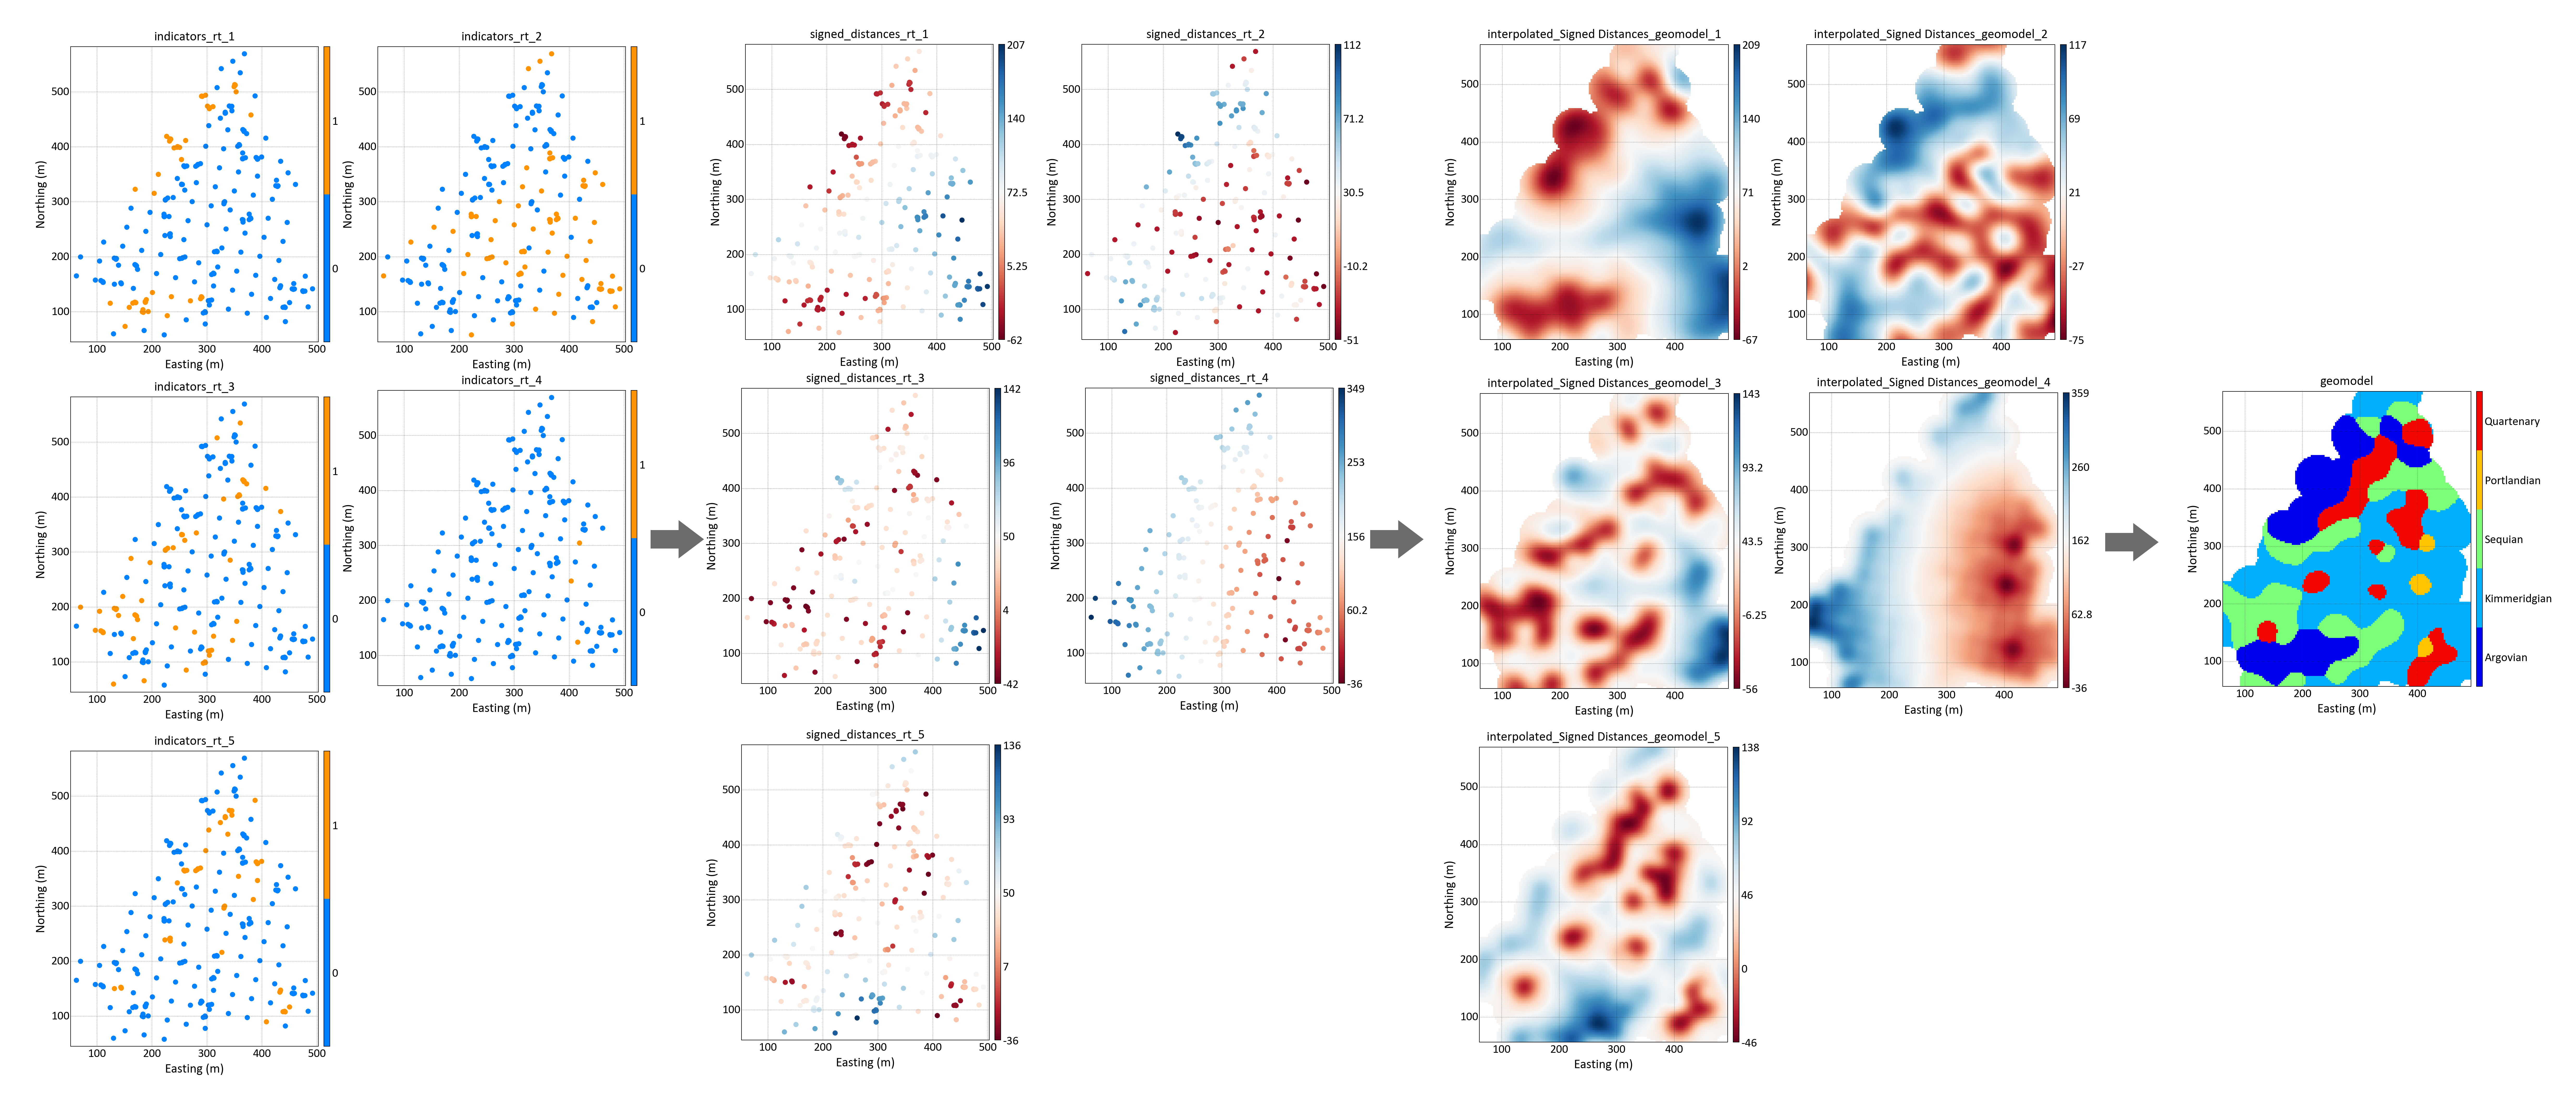
\includegraphics[width=\textwidth]{capitulo_2/imagens/multi category implicit modeling.png}
\end{figure}

A \autoref{multi_alt} mostra as coordenadas das distâncias assinaladas estimadas nos eixos x e y e o valor da distância assinalada no eixo z para cada uma das cinco categorias. Os blocos são classificados com a categoria responsável pela distância estimada "mais negativa".

\begin{figure}[H]
	\centering
	\caption{\label{multi_alt}Uma outra forma de visualizar a modelagem geológica para múltiplas categorias.}
	\subfloat[][Vista 1.]{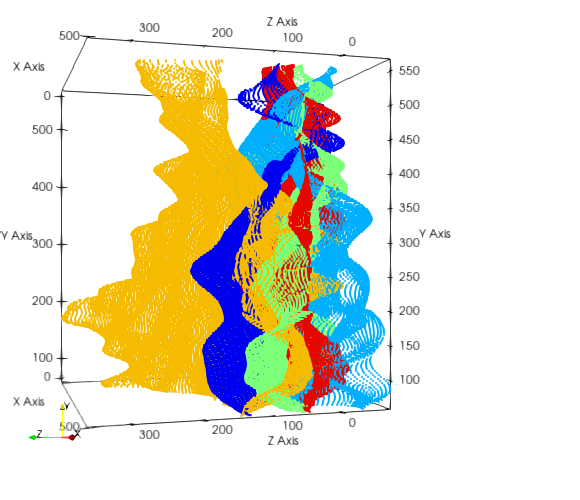
\includegraphics[width=.3\textwidth]{capitulo_2/imagens/multi1.png}\label{<figure1>}}
	\hspace{1em}
	\subfloat[][Vista 2.]{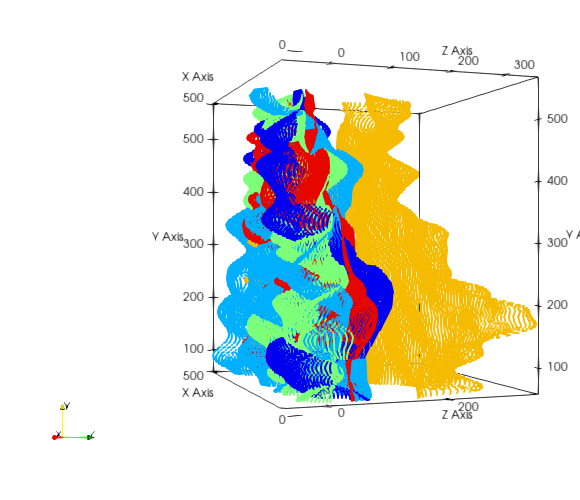
\includegraphics[width=.3\textwidth]{capitulo_2/imagens/multi2.png}\label{<figure2>}}
	\hspace{1em}
	\subfloat[][Vista 3.]{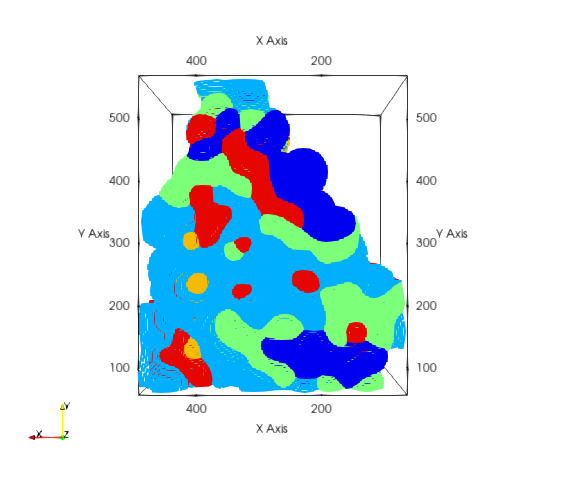
\includegraphics[width=.3\textwidth]{capitulo_2/imagens/multi3.png}\label{<figure3>}}
\end{figure}

\subsubsection{Acelerando o processo}

Embora o uso de métodos globais permita a criação de modelos realistas e livres de artefatos, existem limitações em bancos de dados volumosos já que métodos globais demandam muito processamento e memória RAM. Existem algumas técnicas para superar essa limitação como a solução iterativa \cite{beatson1999fast} por exemplo. Dois métodos que apresentam bons resultados no contexto da modelagem geológica com distâncias assinaladas serão apresentados.

\subsubsubsection{Decomposição do domínio} \label{dom_decomp}

A decomposição do domínio (\textit{Partition of unity - POU}) \cite{wendland2004scattered}, transforma um problema volumoso e que demanda muito esforço computacional em diversos problemas menores e eficientes que são, ao final, unidos.

A demonstração das equações pode ser encontrada em \citeonline{wendland2004scattered} e \citeonline{martin_boisvert_review_rbf}. Um domínio $A$ é subdividido em uma série de partições sobrepostas $\beta$, como mostrado na \autoref{pou} à direita, de modo que a união de todas as $k$ partições em $A$, $\{ \beta \}^K_{j=1}$ compreende o domínio. Para cada partição, os dados correspondentes são utilizados para interpolar a função escalar $s_j(x)$.

A função peso para cada partição deve ser igual a um no centro e 0 na fronteira, a contribuição de cada partição nos locais de sobreposição é dado pela função peso.

As partições são definidas encontrando uma série de coordenadas para seus centros. Diversos métodos podem ser utilizados: um grid regular, k-means, árvore binária, \textit{oct tree}.

A \autoref{pou} mostra um domínio particionado: o particionamento começa considerando o domínio completo como sendo uma partição, então a partição "total"\ é subdividida recursivamente em duas, mantendo um nível de sobreposição. O particionamento termina quando cada partição individual tem menos amostras que o máximo especificado pelo usuário \cite{martin2017implicitmodeling, martin2017iterative}. Dessa forma, áreas com alta densidade amostral ficam em partições pequenas; enquanto, áreas esparsas ocupam partições maiores.

\begin{figure}[H]
	\caption{\label{pou}Particionamento do domínio.}
	\centering
		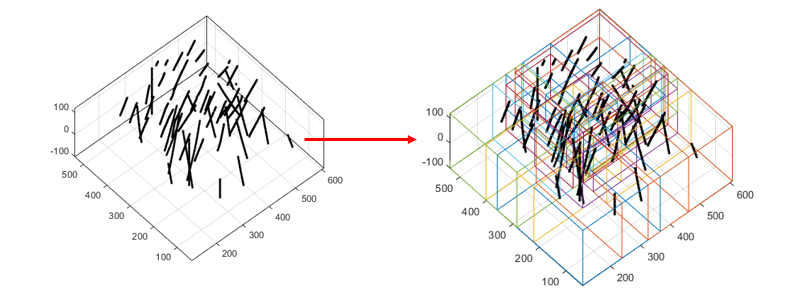
\includegraphics[width=\textwidth]{capitulo_2/imagens/pou.jpg}
	\legend{Fonte: \citeonline{martin2017iterative}}
\end{figure}

Deve haver um número de amostras em cada partição e sobreposição das partições suficientes para evitar o surgimento de artefatos quando as partições independentes forem unidas.

O método deve ser utilizado para um único domínio por vez. Na presença de múltiplos domínios uma regra hierárquica deve ser definida ou a categoria responsável pela menor distância estimada deve ser retida.

\subsubsubsection{Refinamento dos contatos} \label{bound_ref}

\citeonline{silva2015speeding} propuseram uma técnica baseada no algoritmo dos cubos marchantes \cite{lorensen1987marching} para acelerar o processo de modelagem em modelos multi-categóricos. O primeiro passo é criar o modelo geológico usando distâncias assinaladas em um \textit{grid} grosseiro, como mostra o mapa a esquerda na \autoref{refi_cont}. 

Depois disso, o algoritmo dos cubos marchantes é aplicado ao modelo geológico com o objetivo de identificar a região ao redor dos contatos. Neste algoritmo, um cubo composto por 8 células em três dimensões ou 4 células em duas dimensões percorre o \textit{grid}, conforme mostrado na \autoref{marcub}, da esquerda para a direita e de cima para baixo visitando todo o \textit{grid}. O algoritmo verifica se pelo menos um dos nós que constituem o cubo pertence a uma categoria diferente dos demais. Nesse caso, esses blocos são marcados como região de contato. 

\begin{figure}[H]
\caption{\label{marcub} Esquema mostrando o funcionamento do algoritmo cubos marchantes.}
	\centering
		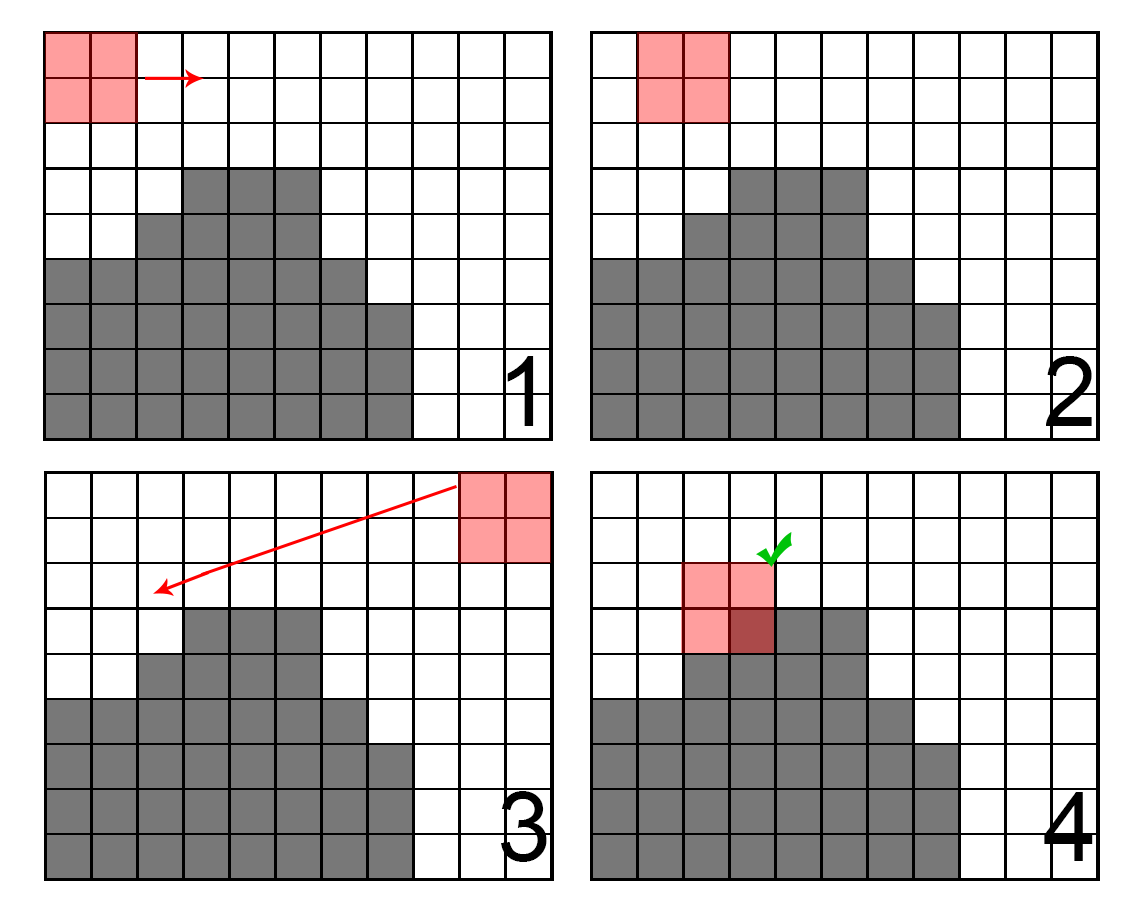
\includegraphics[width=0.6\textwidth]{capitulo_2/imagens/marching_cubes.png}
\end{figure}

Por fim, o \textit{grid} é reduzido (\textit{downscaled}) e uma nova interpolação das distâncias e posterior classificação é realizada apenas nas regiões marcadas como contato. Os demais blocos são classificados com a mesma categoria que pertenciam no modelo no \textit{grid} grosseiro. A posição real do contato necessariamente está localizada na região demarcada pelo algoritmo.

Os passos são repetidos de forma automática, um número de vezes definido pelo usuário, até que a resolução necessária seja atingida.

A \autoref{refi_cont} mostra, seguindo a direção das flechas, o modelo inicial para o \textit{Swiss Jura} criado em um \textit{grid} de dimensões 20x20 m. O algoritmo cubos marchantes então identifica a região dos contatos. Na primeira iteração, as dimensões do \textit{grid} foram reduzidas pela metade, esse parâmetro é escolhido pelo usuário. As distâncias são estimadas no \textit{grid} 10x10 m somente nos blocos marcados como contato pelos cubos marchantes, essa região fica mais estreita a cada iteração. Um novo modelo geológico refinado é criado nesse \textit{grid}. O processo é repetido até que a dimensão dos blocos seja 2.5x2.5 m, como mostrado na imagem da direita na \autoref{refi_cont}.

\begin{figure}[H]
\caption{\label{refi_cont} Esquema mostrando o refinamento dos contatos em três iterações reduzindo as dimensões do \textit{grid} pela metade para o \textit{Swiss Jura}.}
	\centering
		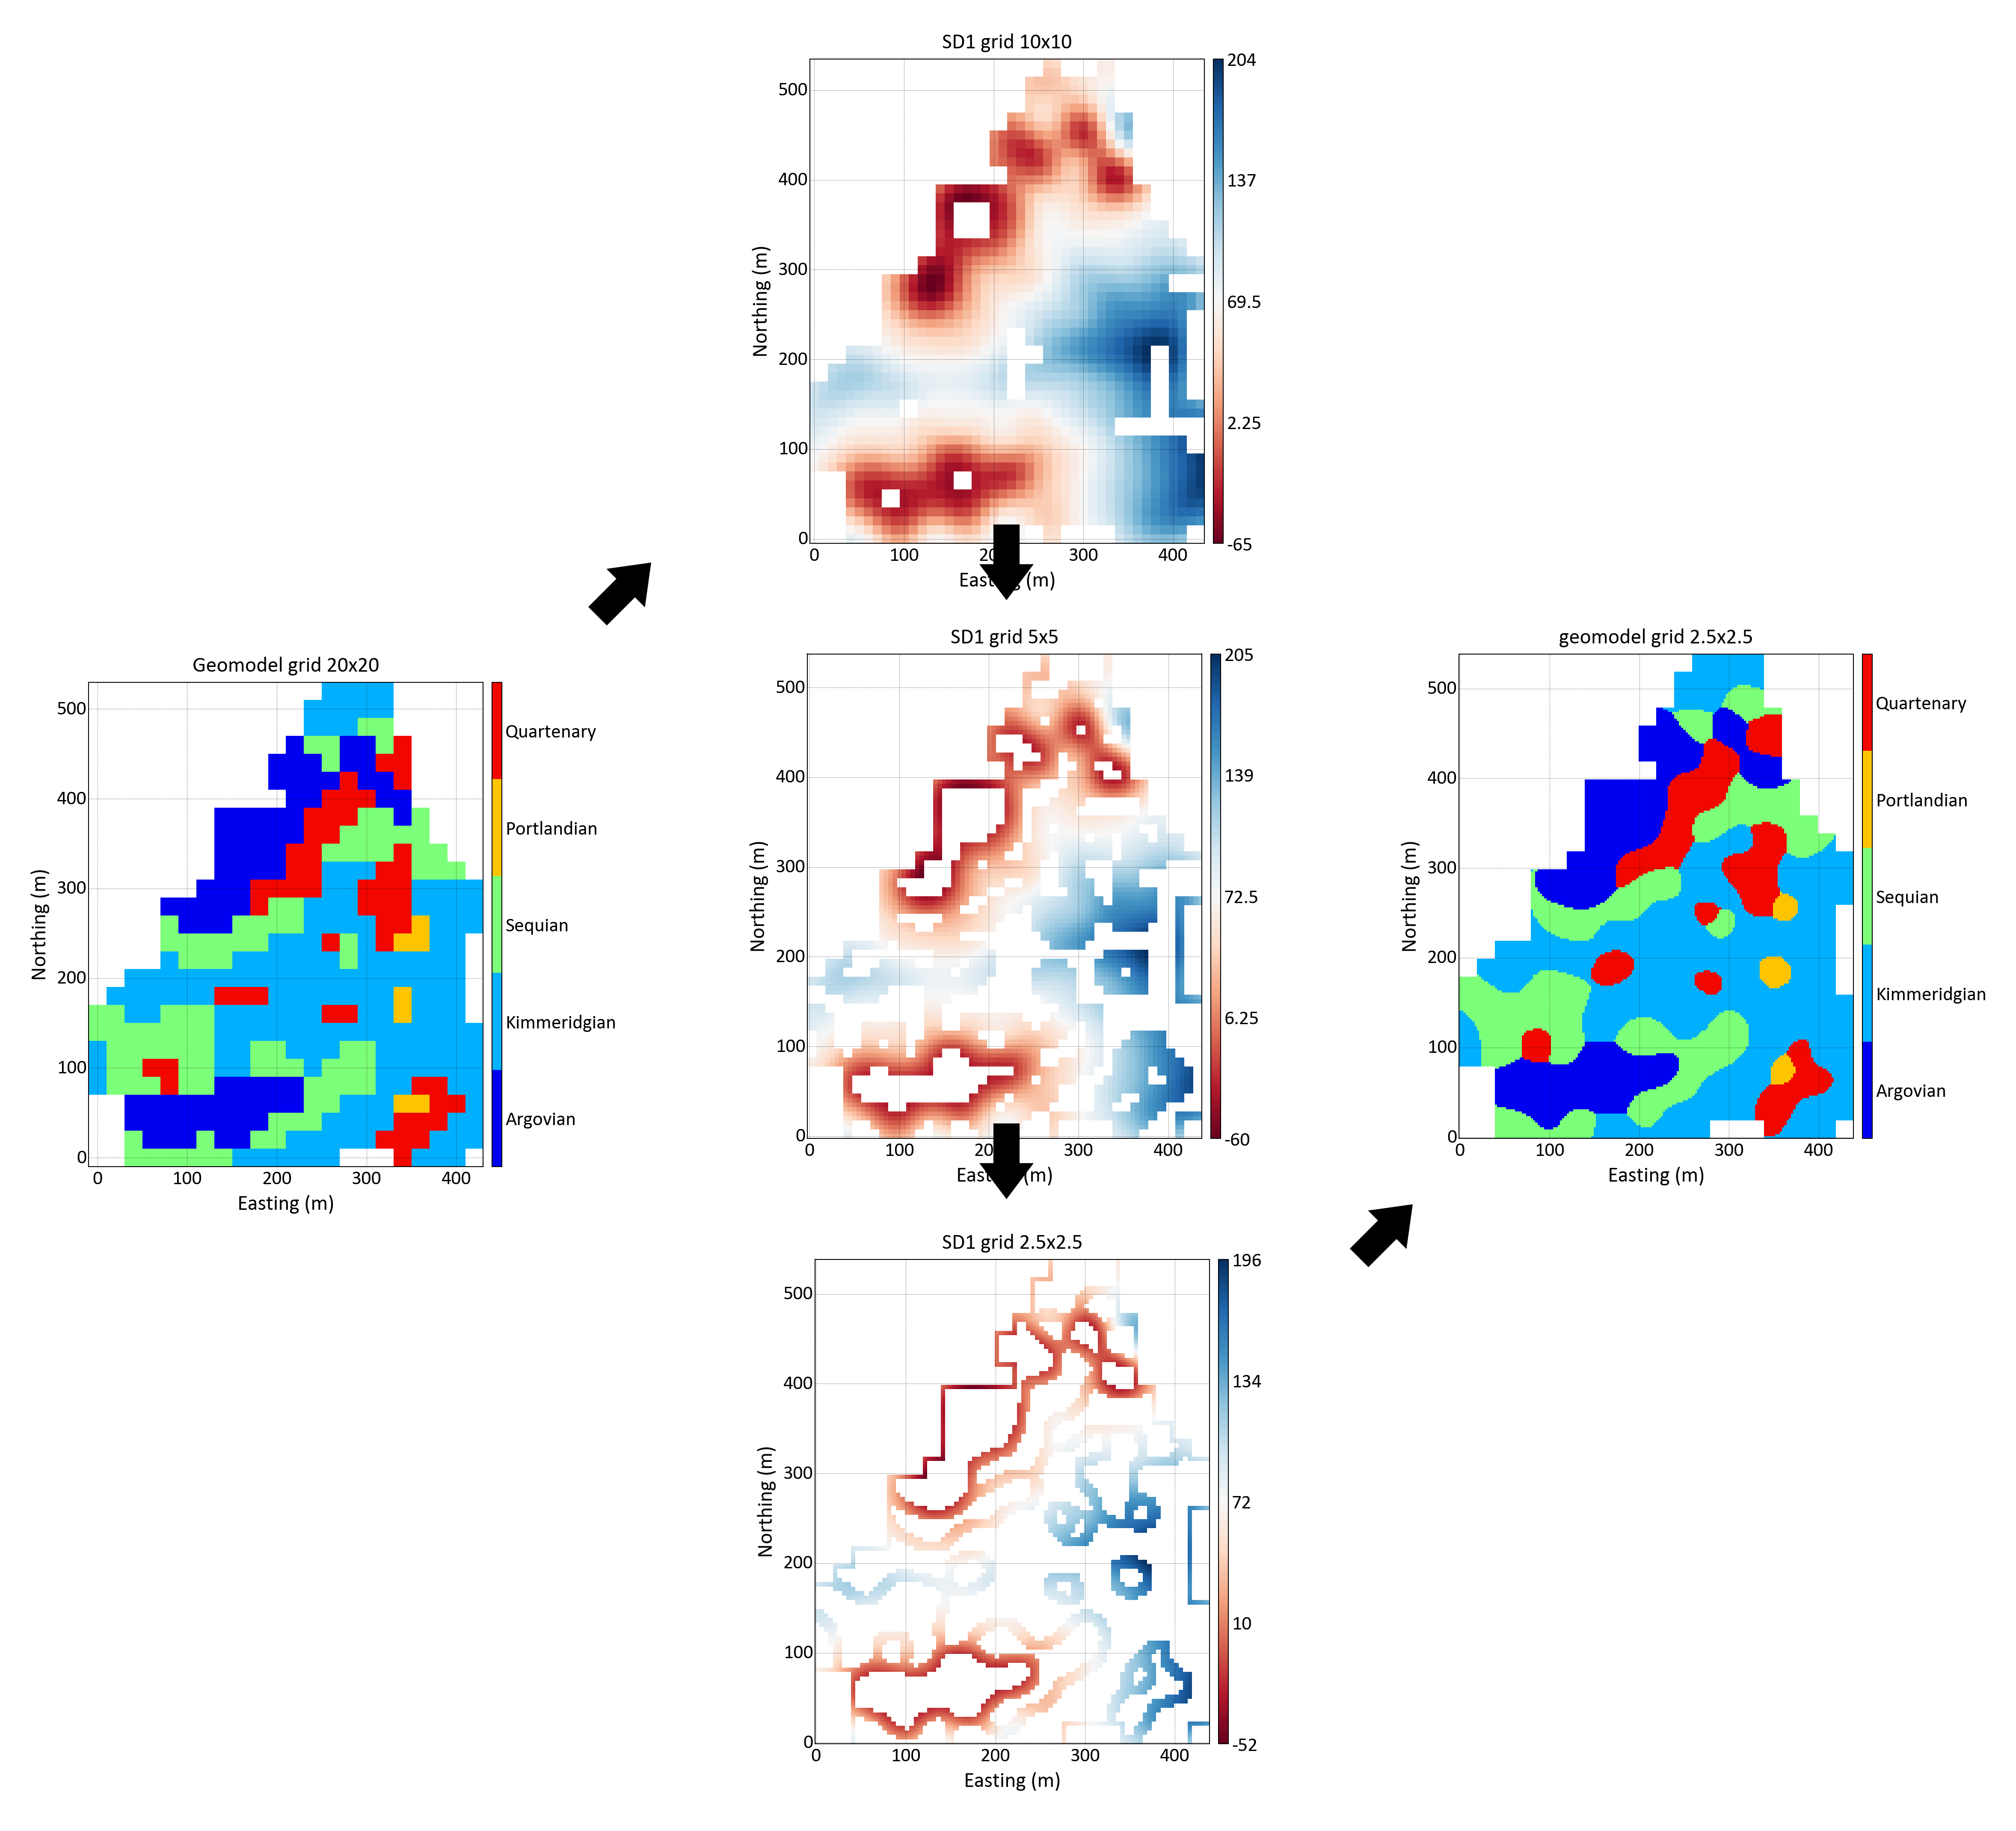
\includegraphics[width=\textwidth]{capitulo_2/imagens/bound_refinement.png}
\end{figure}

\subsubsection{Incorporação de estacionariedade de segunda ordem}

Corpos geológicos são complexos da escala macro à escala micro. Essa característica pode tornar difícil a captura de suas feições com funções de covariância. Segundo \citeonline{martin2017implicitmodeling}, a não estacionariedade de segunda ordem deve ser incorporada quando estruturas complexas estão sendo modeladas.

Anisotropia é definida como o conjunto de rotações e relações anisotrópicas: azimute, mergulho, \textit{rake}, $r1 = \frac{a_{hmin}}{a_{hmax}}$, $r2 = \frac{a_{vert}}{a_{hmax}}$. 

\subsubsubsection{Krigagem com anisotropia local variável}

A krigagem com anisotropia variável exige que os parâmetros locais de anisotropia sejam definidos em todos os nós do grid (\autoref{lva_krig_cartoon}), e variem de forma suave pelo domínio. Isso permite que estruturas curvilineares em escala menor que o espaçamento entre as amostras sejam capturadas \cite{martin2017implicitmodeling}. Porém, torna o método computacionalmente exigente.

\begin{figure}[H]
\caption{\label{lva_krig_cartoon}Esquema mostrando os vetores de anisotropia local e as amostras representadas pelos círculos pretos para cada nó do grid.}
	\centering
		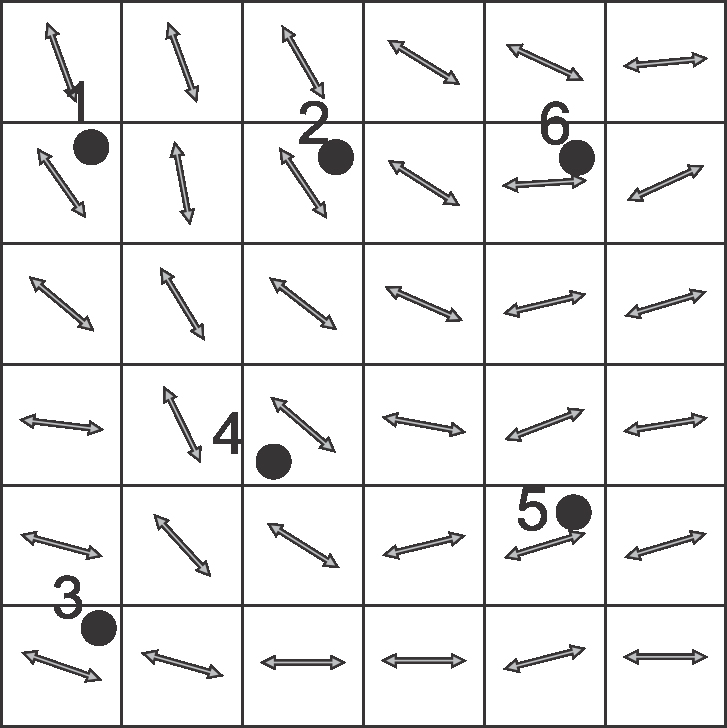
\includegraphics[width=0.6\textwidth]{capitulo_2/imagens/lvakrig.jpg}
	\legend{Fonte: \citeonline{martin2017implicitmodeling}}
\end{figure}

Existem diversos métodos para definição da anisotropia local \cite{lillah2015inference}: pode ser inferida por um geomodelador, estimada diretamente a partir dos dados usando técnicas automáticas, interpolada de uma série de pontos onde a orientação foi medida ou pode ser extraída de dados em um grid que representam a variabilidade local (teores krigados, por exemplo). A biblioteca \textit{GSLib} tem diversos softwares para definição de anisotropia local. 

\subsubsubsection{Funções de bases radiais com anisotropia local variável}

Interpolação com funções de bases radiais com anisotropia local variável é baseada na decomposição de domínios (\autoref{dom_decomp}), um kernel anisotrópico pode ser usado para melhor suportar os dados em cada partição, já que as partições são independentes, uma matriz de rotação é usada para definir \textit{kernels} anisotrópicos locais que melhor se ajustam às propriedades espaciais de cada partição. O interpolador de bases radiais é obtido independentemente para cada partição e a solução final é obtida ponderando as soluções independentes nos locais de sobreposição \cite{martin2017implicitmodeling}.

Ao contrário da krigagem com anisotropia local variável, que requer os vetores de anisotropia em todas os nós do \textit{grid}, a implementação para funções de bases radias requer os vetores somente no centro de cada partição (\autoref{lva_krig_cartoon}) variando suavemente pelo domínio.

\begin{figure}[H]
\caption{\label{lva_rbf+cartoon} Esquema mostrando os vetores de anisotropia local e as amostras, representadas pelos círculos pretos, para cada centro de partição representadas pelas linhas tracejadas vermelhas.}
	\centering
		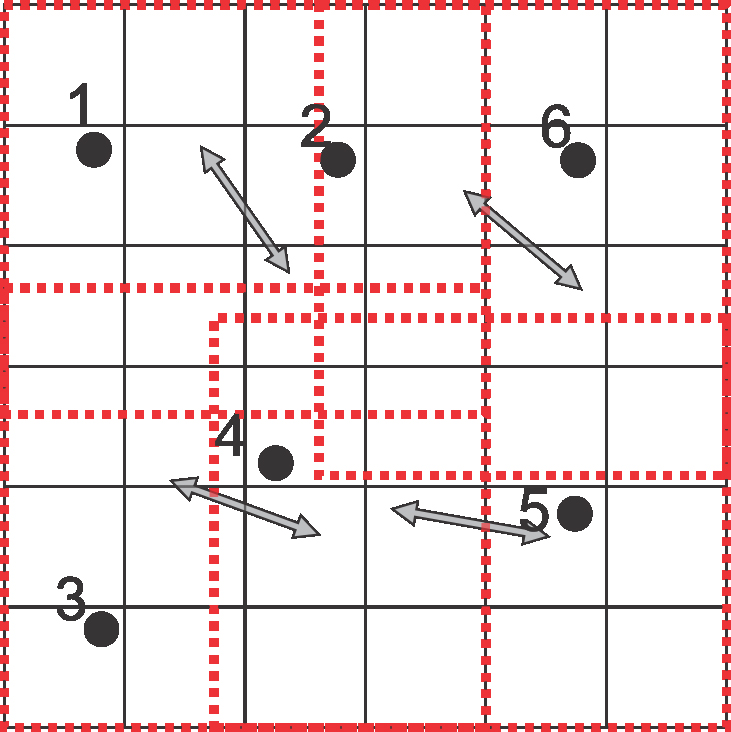
\includegraphics[width=0.6\textwidth]{capitulo_2/imagens/lvarbf.jpg}
	\legend{Fonte: \citeonline{martin2017implicitmodeling}}
\end{figure}

Extrair orientações locais de um modelo criado com anisotropia global e utilizar essas orientações em uma nova interpolação não estacionária resulta em um modelo geológico mais refinado considerando informação local. Esse processo pode ser repetido continuamente refinando o campo de anisotropias locais. 

O refinamento iterativo \cite{martin2017iterative} com funções de bases radiais tem um benefício extra (em relação à krigagem com variação local de anisotropia), a possibilidade de incluir algum tipo de critério de parada, quando o modelo for considerado refinado. Como as partições são independentes, se o refinamento de uma partição em particular não resultar em mudanças significativas, poderá ser omitido na solução final. Essa característica torna o processo significativamente mais rápido \cite{martin2017implicitmodeling}.

A \autoref{iterref} mostra um processo de refinamento iterativo onde a semente é um modelo isotrópico. O algoritmo começa sua execução inferindo orientações anisotrópicas em cada flanco da dobra, que são rasos demais para que sejam definidos adequadamente. Porém, nas próximas iterações do refinamento, o mergulho se torna mais profundo e os flancos são definidos implicitamente.

\begin{figure}[H]
\caption{\label{iterref} Esquema mostrando o refinamento iterativo para funções de bases radiais.}
	\centering
		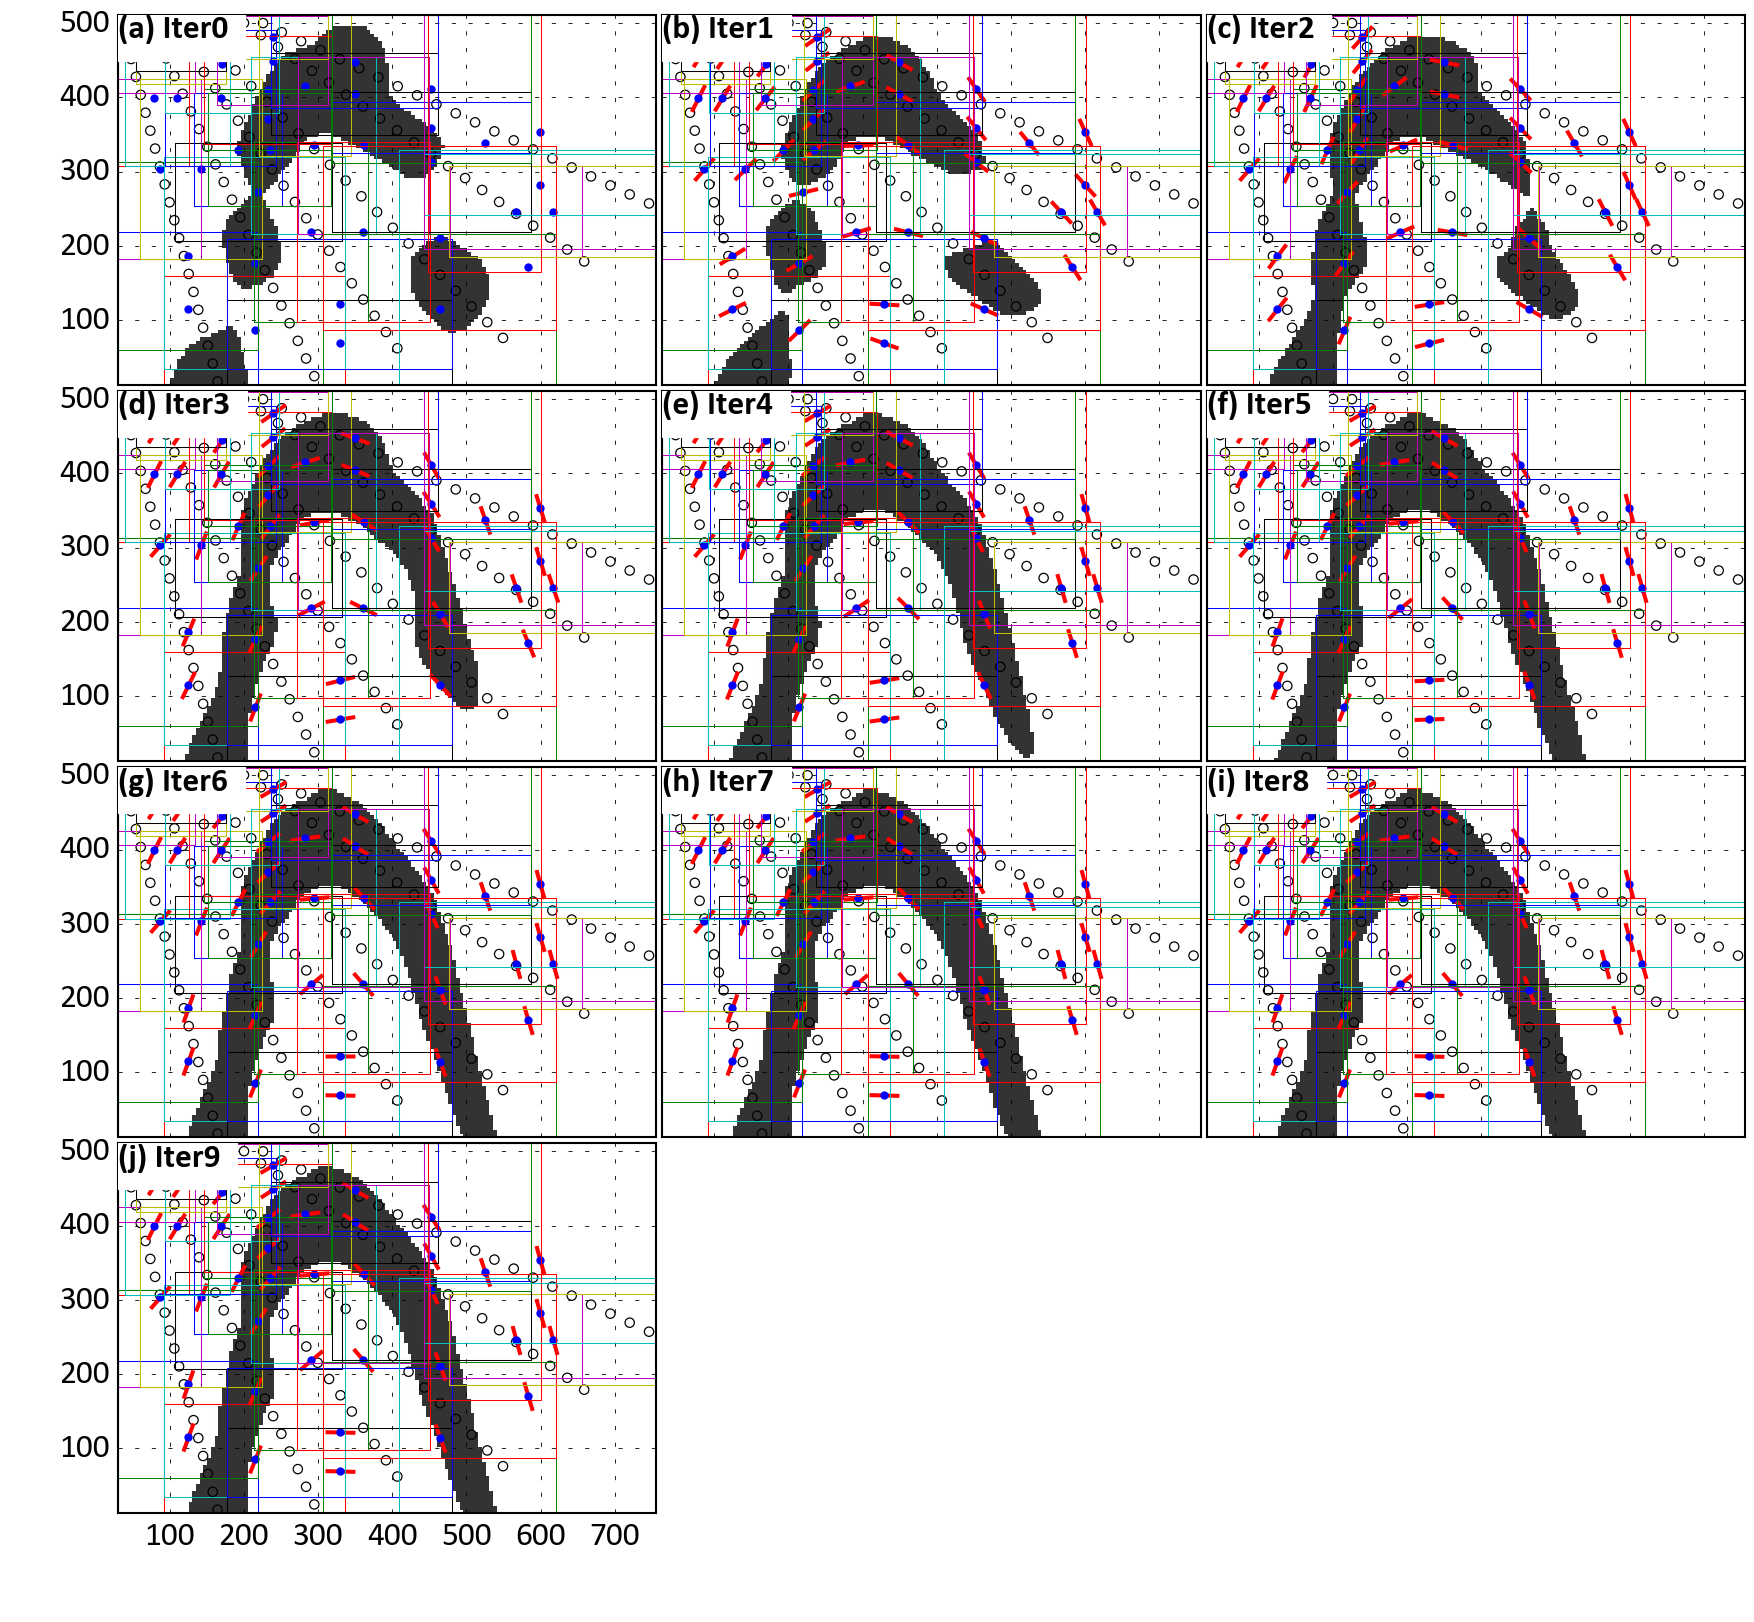
\includegraphics[width=0.6\textwidth]{capitulo_2/imagens/iterref.jpg}
	\legend{Fonte: \citeonline{martin2017iterative}}
\end{figure}

\subsubsection{Desvantagens}\label{problemas}

\citeonline{mancel2019problem} apontam que na presença de dados esparsos e amostras com espaçamento variável, a incerteza em relação à posição dos contatos de um domínio geológico é significativa. Conforme amostras são coletadas e inseridas no modelo, a incerteza em relação à localização diminui e o risco é reduzido. A assimetria espacial na amostragem e a dispersão das amostras são características inerentes às amostragens para avaliação de recursos e podem levar a situações únicas em que as distâncias assinaladas se mostram incapazes de gerar modelos apropriados. 

O problema reside no fato do algoritmo para o cálculo da função distância assinalada buscar a amostra mais próxima codificada com um indicador oposto sem levar em consideração a estrutura e o espaçamento dos dados circundantes. Um cenário unidimensional simples ilustra esse viés devido à assimetria na \autoref{desvant1}. 

A Figura \autoref{desvant11} mostra a situação ideal, onde a amostra amarela da esquerda aponta para a primeira amostra vermelha, da esquerda para a direita. A primeira amostra vermelha aponta para a amostra amarela da esquerda, assim como a segunda amostra vermelha. Já a terceira amostra vermelha aponta para a amostra amarela da direita, dessa forma, o melhor palpite para o limite (ou a isosuperfície zero) da direita entre os domínios amarelo e vermelho se localiza no ponto médio entre as amostras. 

A Figura \autoref{desvant2} mostra a situação que acontece de fato, todas as amostras vermelhas apontam para a amostra amarela da esquerda puxando o limite da direita entre os domínios para perto das amostras vermelhas, diminuindo o tamanho do domínio, ou seja, há um viés conservador no volume dos domínios na presença de forte assimetria nas amostras.

\begin{figure}[H] 
    \centering
    \caption{Cenário unidimensional simples ilustrando o viés devido à assimetria nos modelos geológicos.} \label{desvant1}
     \subfloat[][Situação ideal, sem viés.]{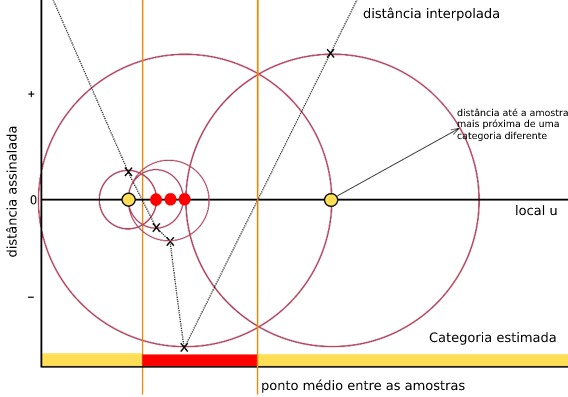
\includegraphics[width=.45\textwidth]{capitulo_2/imagens/sd_prob3.png}\label{desvant11}}
     \hspace{1em}
     \subfloat[][Situação real, com viés conservador.]{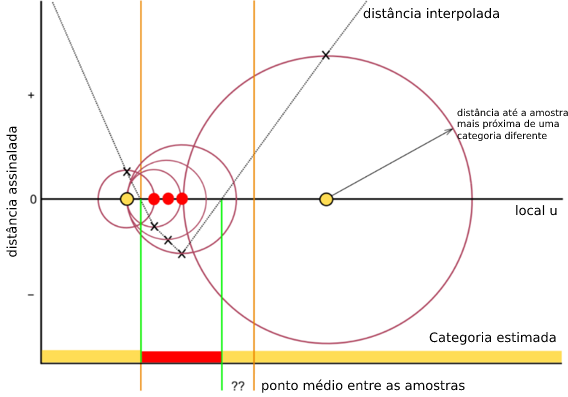
\includegraphics[width=.45\textwidth]{capitulo_2/imagens/sd_prob_2.png}\label{desvant2}}
     \legend{Modificado de \citeonline{mancel2019problem}}
\end{figure}

Os autores propõe uma solução usando indicadores, nesse caso, a isosuperfície definida pela probabilidade de ocorrência 0,5 não é o melhor palpite para a localização do contato. A solução consiste em:

\begin{enumerate}[label=\roman*]
    \item Usar a triangulação de Voronoi para definir a área de influência de cada amostra de indicador;
    \item Calcular a proporção da área total que é ocupada por polígonos que representem amostras do domínio a ser modelado;
    \item Usar a proporção da área (1-p) para definir, a partir da distribuição acumulada da interpolação dos indicadores, o limiar no qual a isosuperfície que represente o contato será extraída. Como mostrado no exemplo da \autoref{nnmet} 
\end{enumerate}.

\begin{figure}[H]
\caption{\label{nnmet} Esquema mostrando a extração da iso-superfície usando indicadores e triangulação de Voronoi. À esquerda a figura mostra o CDF dos indicadores interpolados e em vermelho a proporção (1-0.2) ocupada pelos triângulos que representam amostras no interior do domínio que equivale a um valor de indicador de 0.313. À direita um \textit{cutoff} feito em 0.313 nos indicadores interpolados para definir os limites do domínio.}
	\centering
		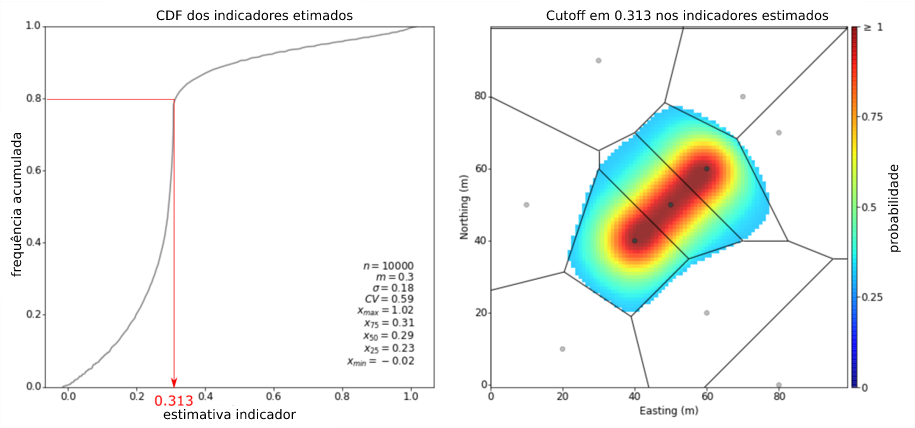
\includegraphics[width=0.8\textwidth]{capitulo_2/imagens/nnmet.png}
	\legend{Modificado de \citeonline{mancel2019problem}}
\end{figure}

\section{Modelagem geológica estocástica}

A necessidade de avaliação da incerteza associada ao modelo geológico impulsionou o desenvolvimento de métodos estocásticos baseados em múltiplas realizações equiprováveis de um atributo. Esses métodos podem ser divididos em dois grupos: métodos baseados em objetos e métodos baseados em células. 

Os métodos baseados em objetos \cite{pyrcz2014geostatistical} têm como objetivo a reprodução da morfologia do depósito, como canais meandrantes em um meio fluvial por exemplo. Geralmente os modelos não são condicionados às amostras. Métodos baseados em objetos ainda não têm muita aplicação na mineração encontrando uso na modelagem de depósitos de óleo e gás.

Os métodos baseados em células, em contrapartida, são condicionados pelas amostras e são utilizados amplamente pela indústria da mineração. Um dos principais métodos desse grupo é a simulação sequencial dos indicadores \cite{alabert1987stochastic}. O algoritmo é robusto e proporciona uma maneira simples e direta de incorporar a incerteza em modelos geológicos multi-categóricos. Entretanto, os modelos podem apresentar uma aparência ruidosa e não realista do ponto de vista geológico \cite{deutsch2006sequential}.

Na simulação sequencial dos indicadores, os nós do \textit{grid} são visitados segundo um caminho aleatório. Uma distribuição condicional de probabilidades é construída em cada nó do \textit{grid,} a partir das amostras e dos nós previamente simulados dentro de um raio de busca. Então, uma categoria é amostrada aleatoriamente da distribuição e atribuída àquele nó.  

Um outro método que se baseia no mesmo princípio é a simulação geostatística multi-ponto (MPS). Esse método utiliza imagens de treinamento para construir a distribuição condicional de probabilidades em cada nó do \textit{grid}. Cada realização deve reproduzir as características geológicas da imagem de treinamento. O método foi inicialmente proposto por \citeonline{guardiano1993multivariate}, porém, diferentes variantes foram desenvolvidas ao longo do tempo \cite{strebelle, boucher2009considering}.

Há ainda a família dos métodos Gaussianos truncados. Esses métodos são aplicados, geralmente, quando as litologias ocorrem em uma ordem fixa, como em sequências estratigráficas por exemplo. A ideia básica por trás da simulação Gaussiana truncada \cite{matheron1987conditional} é simular uma variável Gaussiana em cada célula do \textit{grid} e então aplicar uma regra de truncagem para converter os valores Gaussianos contínuos em valores categóricos.

Em muitos casos, a abordagem Gaussiana truncada se mostra bastante restritiva. Por esse motivo, a técnica pode ser estendida para duas ou mais variáveis Gaussianas. Essa adaptação é chamada de simulação pluri-Gaussiana truncada \cite{armstrong2011plurigaussian}.

O conceito de usar a regra de truncagem em mais de uma dimensão para transformar múltiplas variáveis Gaussianas em uma única variável categórica é limitada, já que a interpretação geológica se degrada quando um número maior de categorias e/ou variáveis gaussianas são consideradas devido à complexidade do modelo.

Por isso, uma nova adaptação foi desenvolvida: \citeonline{silva2019multivariate} propuseram a simulação pluri-Gaussiana truncada hierárquica. Esse método utiliza uma estrutura em árvore para definir diferentes regras de truncagem em uma única dimensão. Isso facilita a definição do mapeamento entre espaço contínuo (Gaussiano) e categórico, tornando possível a utilização eficiente de qualquer número de variáveis Gaussianas para a modelagem de uma variável categórica.

No braço dos métodos implícitos, alguns autores desenvolveram técnicas para avaliar a incerteza dos modelos geológicos. Avaliar a incerteza em relação à posição dos contatos a partir dos campos potenciais é uma  processo direto. \citeonline{gonccalves2017machine} deram uma abordagem de aprendizagem de máquinas para o método possibilitando a avaliação de incerteza. \citeonline{de2019gempy} desenvolveram uma ferramenta de modelagem geológica estocástica de código aberto que avalia a incerteza usando campos potenciais combinados com uma abordagem Bayesiana.

Outros autores construíram modelos implícitos e avaliaram a incerteza do modelo geológico usando dados estruturais. \citeonline{lindsay2012locating} examinaram a incerteza introduzida pelos dados de orientação geológica, produzindo um conjunto de modelos 3D implícitos gerados a partir de medições de orientação sujeitas a simulações de incerteza. \citeonline{pakyuz2018monte} estudaram o efeito da propagação da incerteza dos dados estruturais de entrada na modelagem geológica 3D implícita. \citeonline{caumon2007elements} avaliaram a incerteza do modelo geológico ao perturbar os parâmetros geológicos, como superfícies de falha e horizonte de alteração.

Também existem na literatura métodos de avaliação de incerteza baseados em distâncias assinaladas, as próximas seções apresentam os principais. Alguns desses, que são base para alguns dos métodos propostos no \autoref{chap3}, serão abordados com mais profundidade.

\subsection{Avaliação heurística da incerteza}\label{heuristic}

O método mais simples de avaliação de incerteza em modelos geológicos implícitos, proposto por \citeonline{silvaanddeutschccgmodeling}, consiste em transformar distâncias estimadas em probabilidades via \textit{softmax transformation}. Técnica amplamente usada em métodos de classificação para múltiplas classes \cite{mccullaghgeneralizedlinear}. A ideia é transformar as distâncias estimadas em probabilidades a partir da \autoref{eq_softmax}. Os valores transformados encontram-se entre zero e um e sua soma deve ser igual a um, para cada bloco em que as distâncias assinaladas forem estimadas.

\begin{equation}
	P(i(u)=k)=\frac{e^\frac{-d^*_k(u)}{\omega}}{\sum_{k'=1}^{K}e^\frac{-d^*_k(u)}{\omega}}
    \label{eq_softmax}
\end{equation}

$P(i(u)=k)$ representa a probabilidade de um local $u$ pertencer à categoria $k$, $d^*_k(u)$ é a distância estimada para a categoria $k$ e $\omega$ é um parâmetro que regula a inter-relação entre as probabilidades das $K$ diferentes categorias. Quanto maior $\omega$, maior as diferenças entre as probabilidades (maior a banda de incerteza). \citeonline{silvaanddeutschccgcorrecting} advogam que o parâmetro pode ser o maior módulo entre as distâncias estimadas em um nó. 

A \autoref{softmax_grafico} mostra, à esquerda, as distâncias estimadas em uma determinada célula do \textit{grid} criado para a modelagem do \textit{Swiss Jura} e a direita as distâncias transformadas em probabilidades usando a \autoref{eq_softmax}. O parâmetro $\omega$ é o maior módulo entre as distâncias estimadas naquele bloco.

\begin{figure}[H]
	\caption{\label{softmax_grafico}Distâncias estimadas e transformadas em probabilidades para um mesmo bloco do \textit{Swiss Jura}}
	\centering
		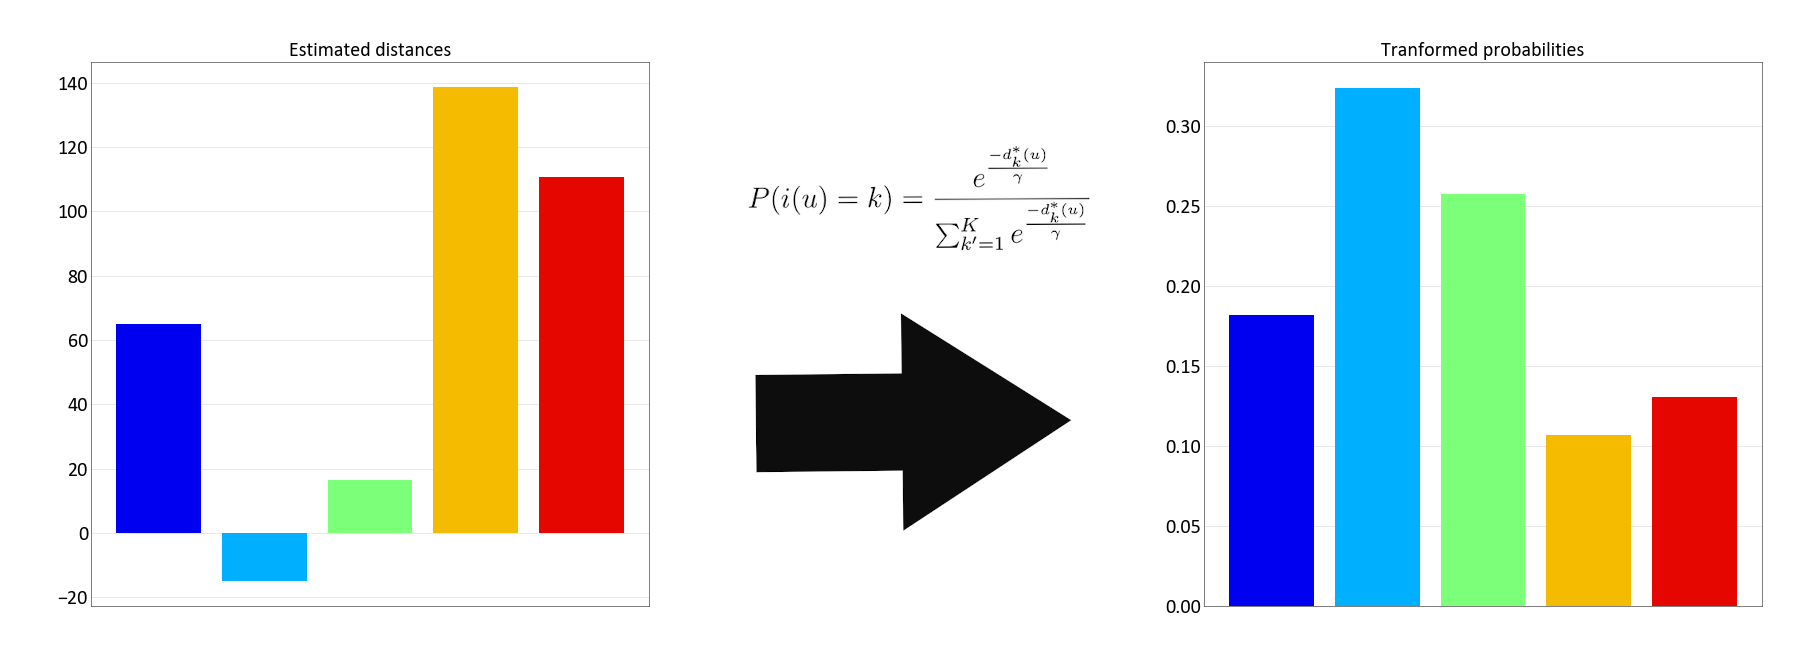
\includegraphics[width=0.7\textwidth]{capitulo_2/imagens/dis_to_probs.png}
\end{figure}

A \autoref{omega_ent} mostra a relação entre $\omega$ e a entropia de Shannon \cite{shannon1948mathematical} calculada pela \autoref{shannon_entr} para o bloco da \autoref{softmax_grafico}. $P(X_k)$ é a probabilidade para a categoria k. Para pequenos valores de $\omega$, uma das categorias será transformada em uma probabilidade muito alta, enquanto as outras serão transformadas em probabilidades muito baixas, nesse caso a entropia é mínima. À medida que o parâmetro $\omega$ aumenta, a diferença entre as probabilidades torna-se menos pronunciada até que a probabilidade para todas as categorias seja igual, caso em que a entropia é maximizada.

\begin{equation}
	H(X)=-\sum_{k=1}^{K}P(X_{k})log(P(X_{k}))
    \label{shannon_entr}
\end{equation}

\begin{figure}[H]
\caption{\label{omega_ent} Relação entre o parâmetro $\omega$ e a entropia de Shannon.}
	\centering
		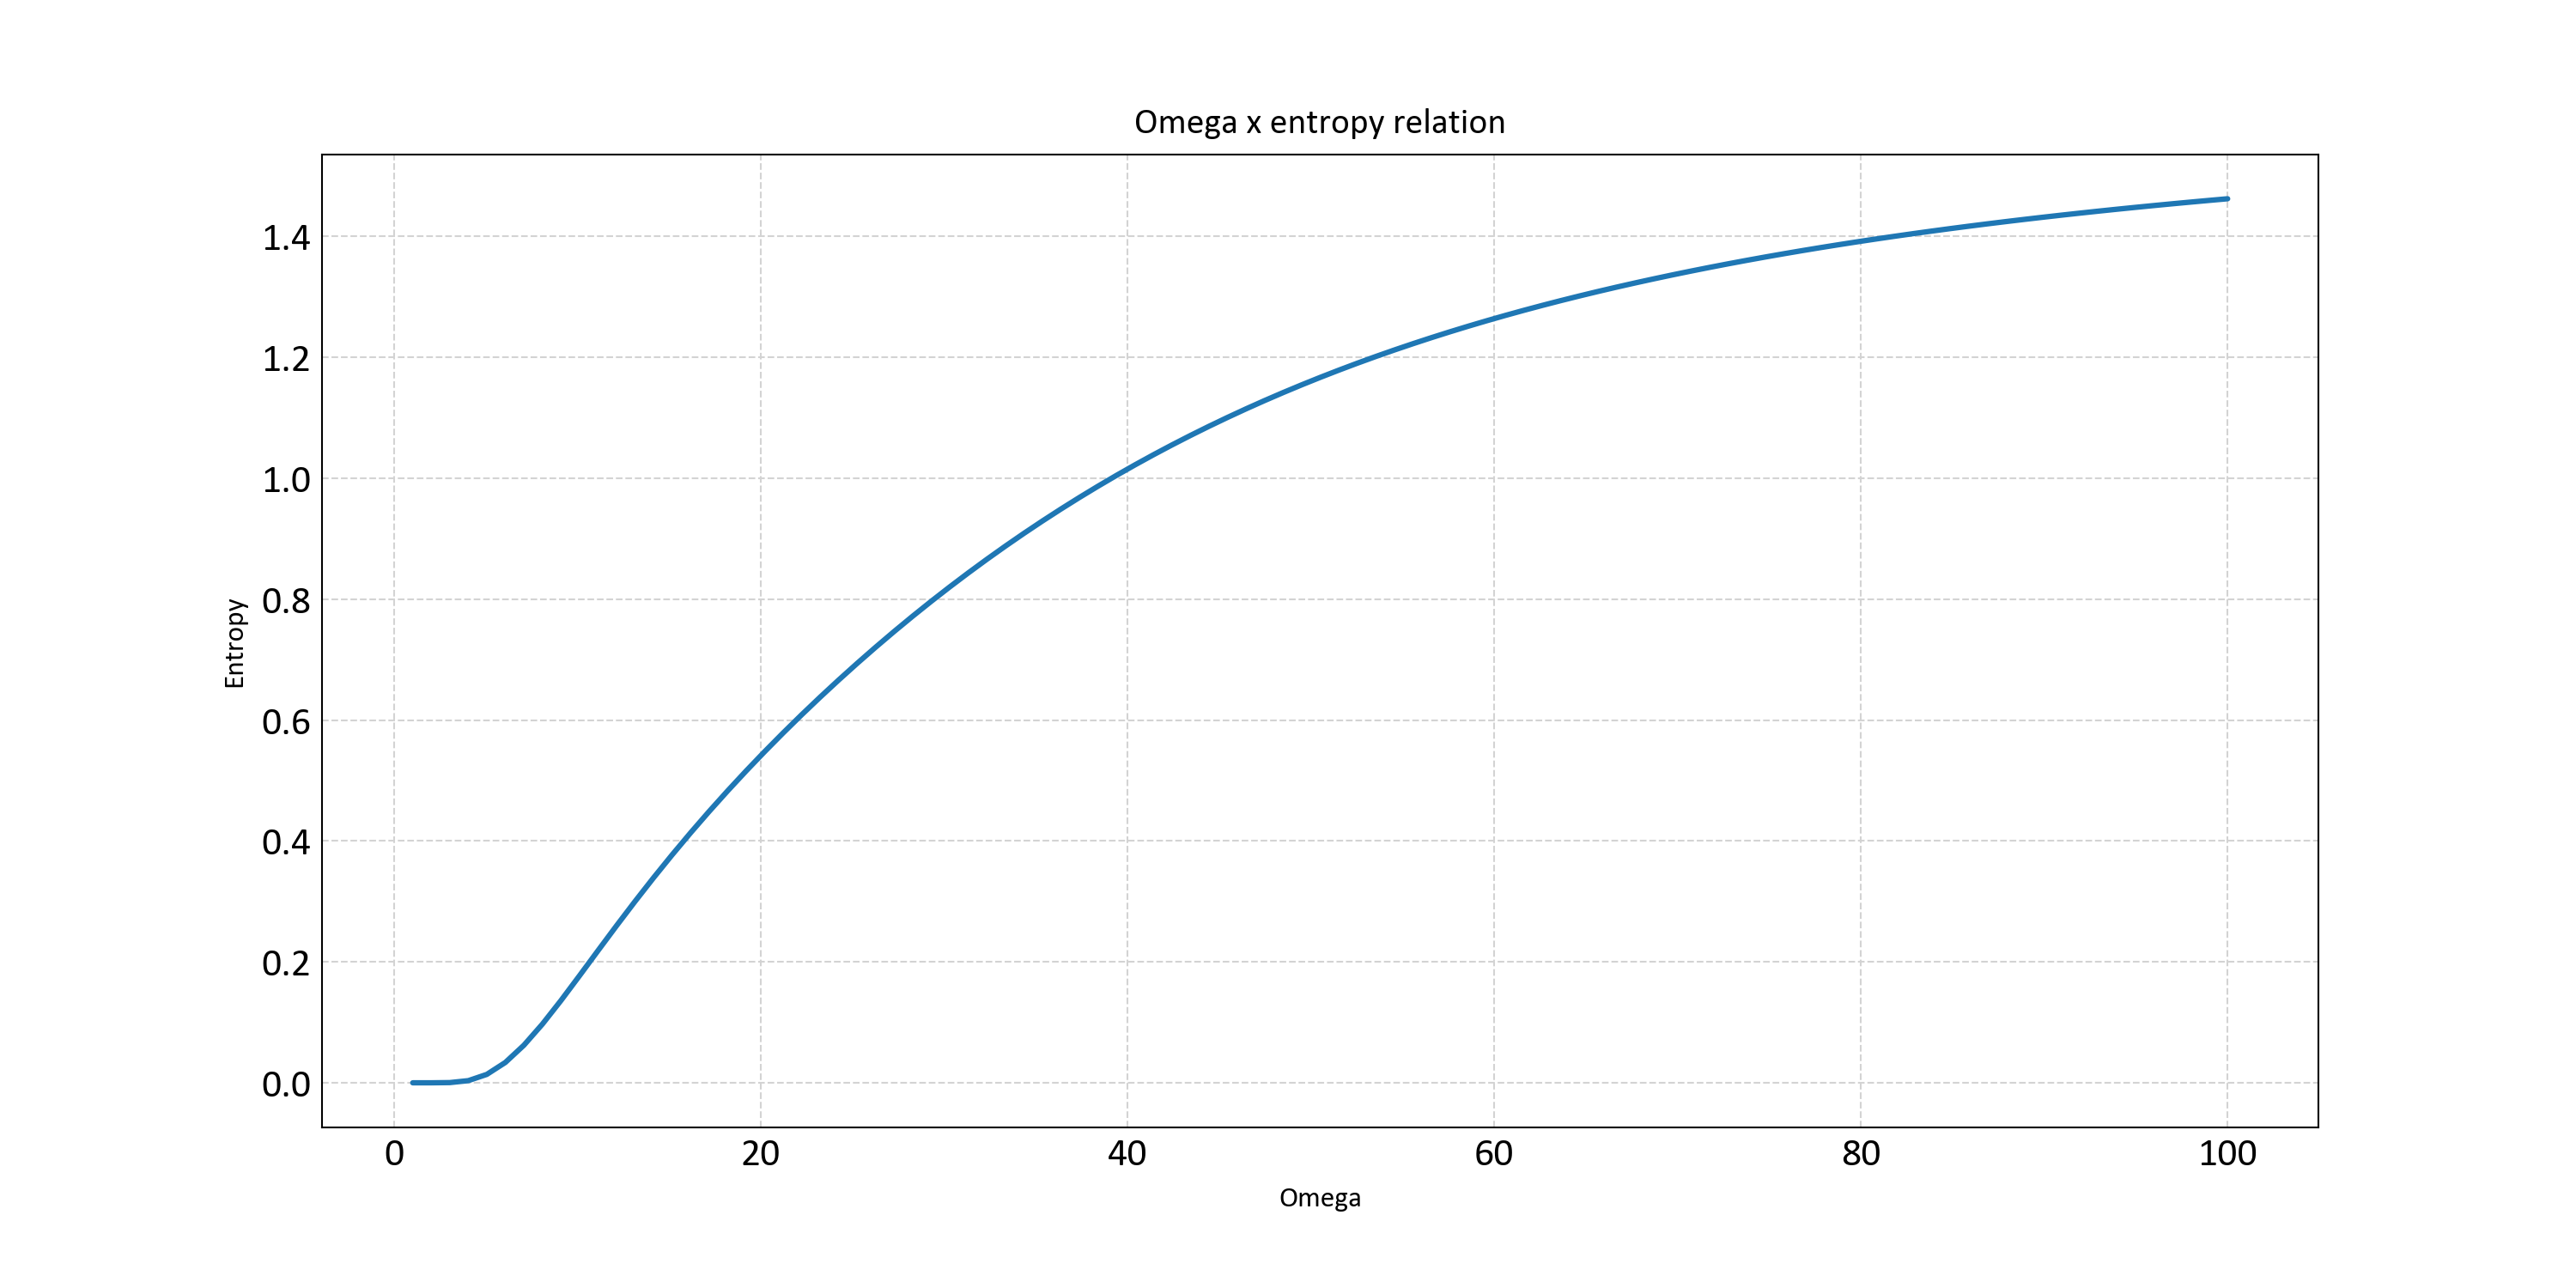
\includegraphics[width=0.8\textwidth]{capitulo_2/imagens/omega_entropy.png}
\end{figure}

A \autoref{jura_prob} mostra, à esquerda, as probabilidades para a categoria Quaternary obtidas transformando as distâncias assinaladas com o valor de $\omega$ igual a 10. Para esse valor do parâmetro há muitas regiões com probabilidade zero ou um de ocorrência e algumas regiões de transição próximas aos contatos. Ao centro, as probabilidades calculadas a partir das distâncias para $\omega$ igual a 100, nesse caso, há uma menor diferença entre as probabilidades. Por fim, à direita, as probabilidades foram calculadas usando como parâmetro $\omega$ o maior módulo entre as distâncias estimadas.

\begin{figure}[H] 
    \centering
    \caption{Distâncias transformadas em probabilidades para a categoria Quaternary usando valores diferentes para $\omega$.} \label{jura_prob}
     \subfloat[][$\omega = 10$.]{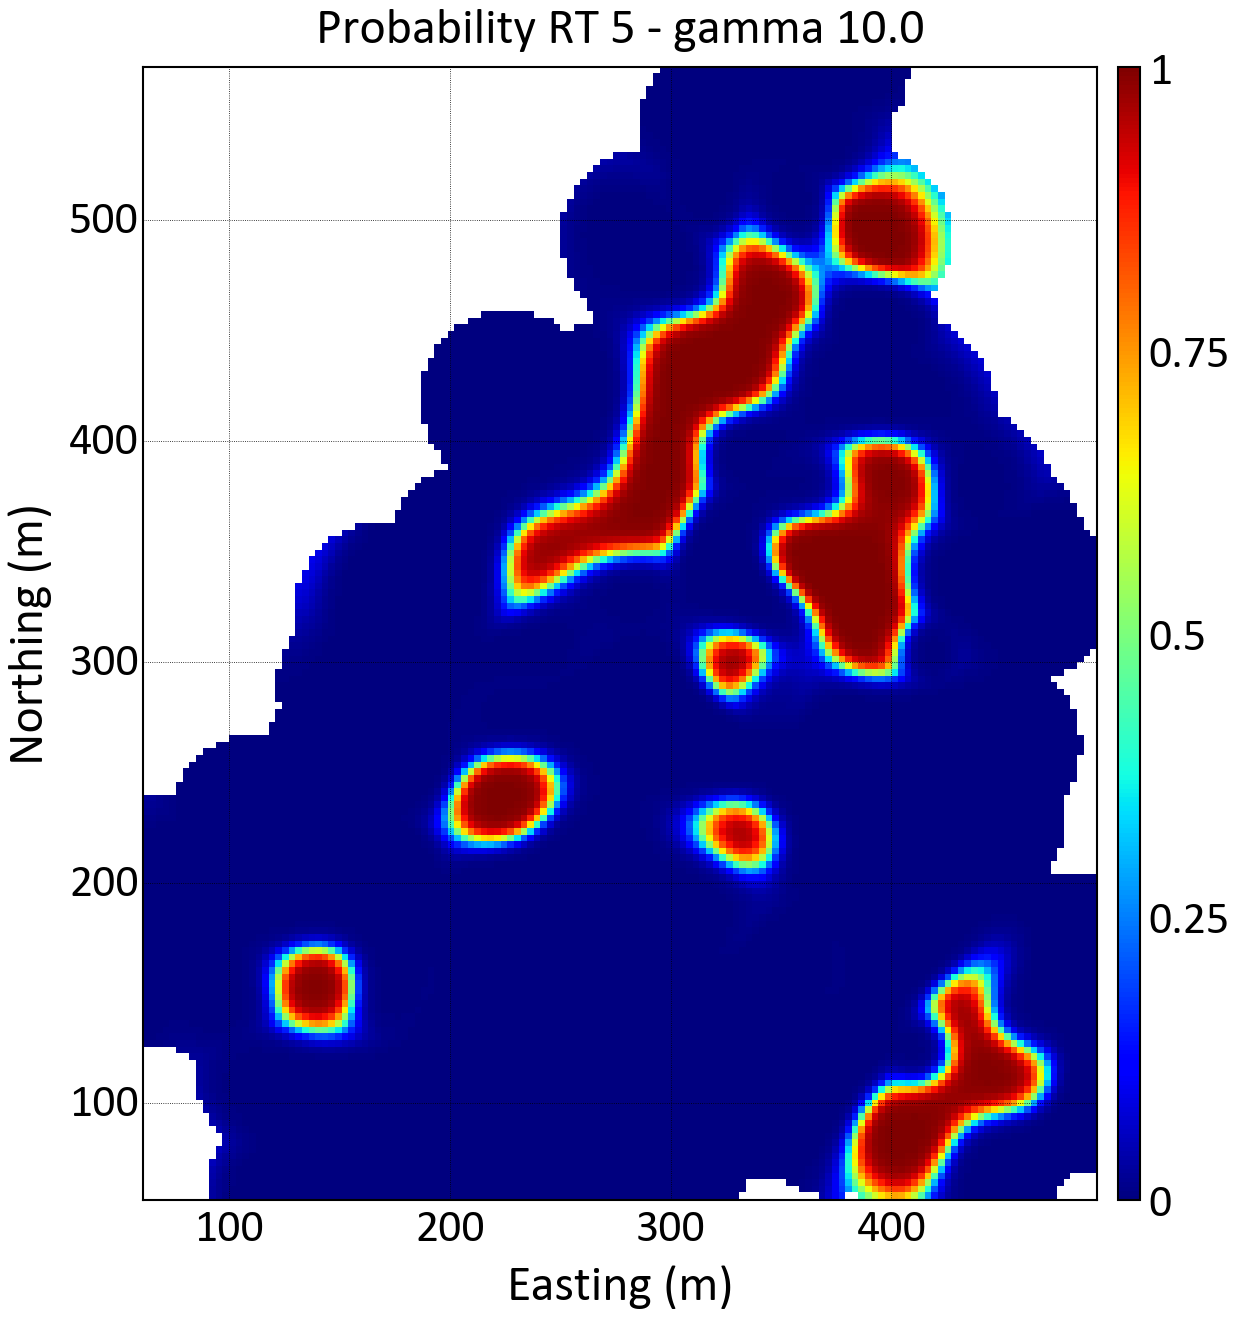
\includegraphics[width=.3\textwidth]{capitulo_2/imagens/probs_10.0.png}\label{<figure1>}}
     \hspace{1em}
     \subfloat[][$\omega = 100$]{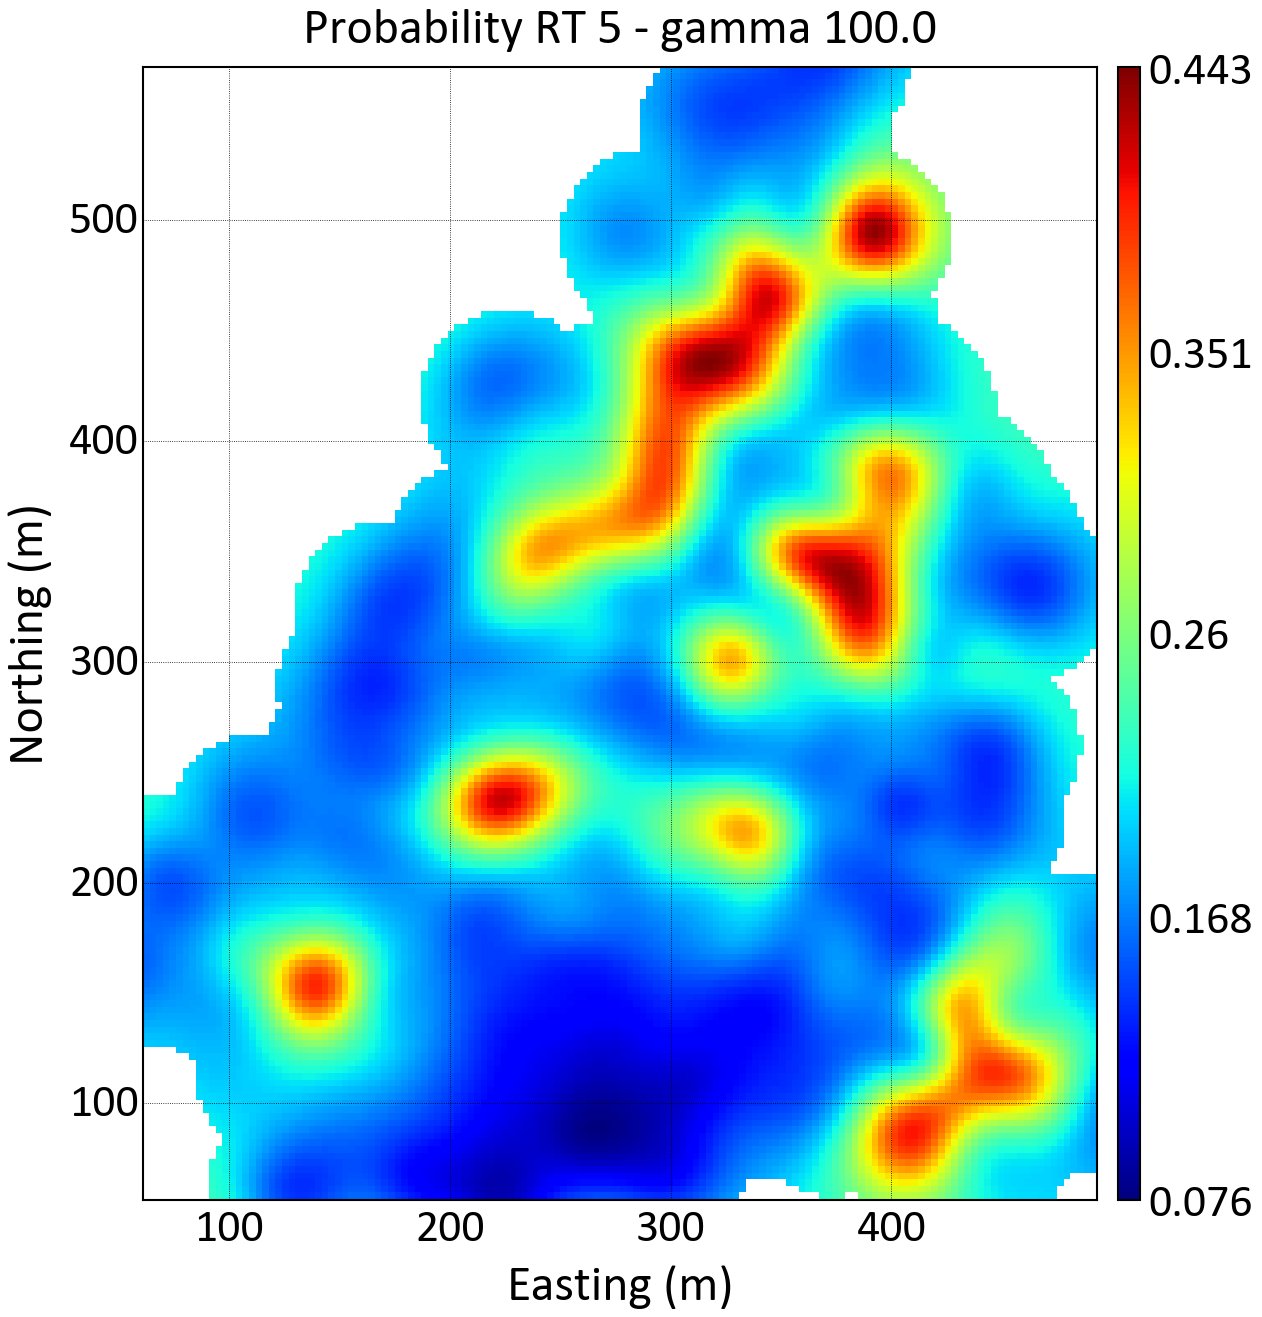
\includegraphics[width=.3\textwidth]{capitulo_2/imagens/probs_100.0.png}\label{<figure2>}}
     \hspace{1em}
     \subfloat[][$\omega = $ maior módulo entre as distâncias estimadas.]{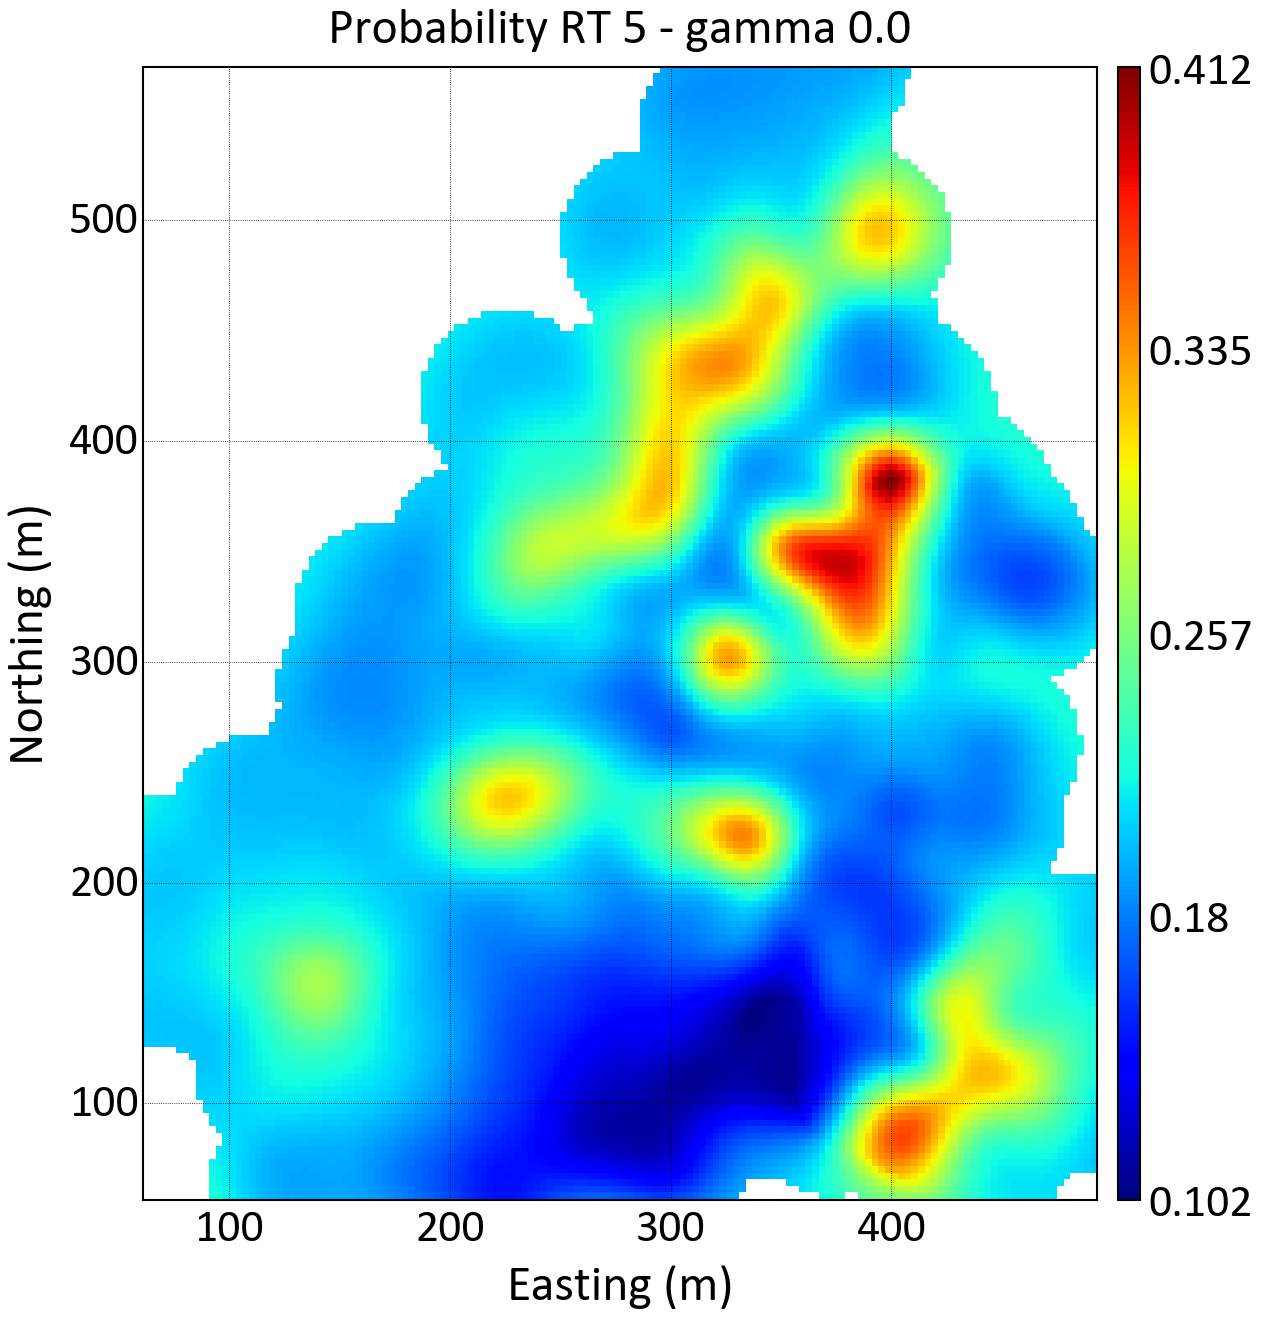
\includegraphics[width=.3\textwidth]{capitulo_2/imagens/probs_0.0.png}\label{<figure3>}}
\end{figure}

Apesar do método ser simples e direto, suportar múltiplas categorias simultaneamente, seu resultado não pode ser utilizado em etapas subsequentes do processo de  avaliação de recursos, por não gerar múltiplas realizações do modelo geológico.

\subsection{\textit{Boundsim}}

Uma outra metodologia proposta por \citeonline{mclennanstationarity, mclennan2006boundsim} consiste em realizar um \textit{bootstrap} espacial \cite{deutsh_spatial_bootstrap} da média da distância assinalada calculada para uma dada categoria. O procedimento de \textit{bootstrap} é amplamente utilizado para quantificar incerteza em parâmetros estatísticos. As duas mais importantes suposições são: os dados são representativos e os dados são independentes. Por esse motivo, a técnica de amostragem deve ser modificada para variáveis que apresentam continuidade espacial. 

Diferentes valores para a média são tomados do histograma da média da distância assinalada, gerado pelo \textit{bootstrap} espacial. Esses valores podem ser correspondentes ao p10, p50 e p90 por exemplo. Então, as distâncias assinaladas são interpolados para os nós do \textit{grid} por krigagem simples, que tem como hipótese a estacionariedade da média por todo o domínio. A média estacionária para a krigagem simples são os valores tomados do histograma.

O último passo consiste em extrair a isosuperfície zero dos modelos implícitos gerados por krigagem simples com os diferentes valores da média estacionária tomadas do histograma da média. Em tese, quanto maior o percentil menor o risco associado, o volume do sólido modelado expande ou contrai de acordo com o valor escolhido para a média estacionária.

A metodologia é simples e direta, porém, deve ser aplicada à uma categoria por vez, na presença de múltiplos domínios alguma abordagem hierárquica deve ser estabelecida. A sensibilidade da krigagem simples à média depende da configuração espacial das amostras, muitas vezes a diferença entre os volumes obtidos é irrelevante.

O produto final do método pode ser utilizado nas etapas subsequentes do processo de avaliação, todavia, o método não avalia incerteza de forma adequada. Os autores do estudo original aplicaram a metodologia apenas em bancos de dados sintéticos e de geometria regular. 

\subsection{Condicionamento das amostras}\label{chap:cond_amo}

\citeonline{mclennanstationarity} também propôs uma metodologia baseada na parametrização das amostras e posterior estimativas. Os pesos de krigagem e da interpolação pelo inverso da distância dependem do arranjo geométrico das amostras mas não dos valores das amostras. A proposta é alterar os pesos dados às amostras a partir de um fator de condicionamento $f^{DC}_i(u)$, como apresentado na \autoref{estimador_cond}

\begin{equation}
\label{estimador_cond}
d^*(u)=\sum_{i=1}^{n} f^{DC}_i(u) \lambda_i(u) d(u_i)
\end{equation}

Onde $d^*(u)$ é a distância interpolada no local não amostrado $u$, $d(u_i)$ são as distâncias assinaladas calculadas para as amostras, $\lambda_i(u)$ são os pesos dados pela krigagem ou inverso da distância e $f^{DC}_i(u)$ são os fatores de condicionamento que dependem do valor numérico das amostras. A krigagem ou inverso da distância clássicos apresentam um fator de condicionamento igual a um para todas as amostras.

Limites pessimistas ou otimistas podem ser gerados a partir das parametrizações mostradas na \autoref{param}. A reta de inclinação negativa da Figura \autoref{paramlinear} dá cada vez mais peso para amostras de distância mais negativas, e cada vez menos peso para amostras mais positivas produzindo uma isosuperfície zero otimista. O domínio tem um volume maior em relação ao caso base onde $f^{DC}_i(u)$ é igual a um para todas as amostras independente do seu valor. O contrário acontece para a reta com inclinação positiva. 

A magnitude da diferença entre os limites otimistas e pessimistas é dada pelo parâmetro fator mínimo, ou \textit{fmin}, escolhido pelo usuário. Um f mínimo igual a um, gera um fator igual a um para todas as amostas (estimativa clássica). Quanto maior o fator, maior a inclinação da reta, e consequentemente, maior a diferença entre os cenários. O valor de f mínimo pode ser diferente para os cenários otimista e pessimista.

A magnitude da diferença pode ser acentuada usando uma função quadrática (Figura \autoref{paramquadrat}) ao invés de uma linear.

\begin{figure}[H] 
    \centering
    \caption{Parametrização das amostras.} \label{param}
     \subfloat[][Linear.]{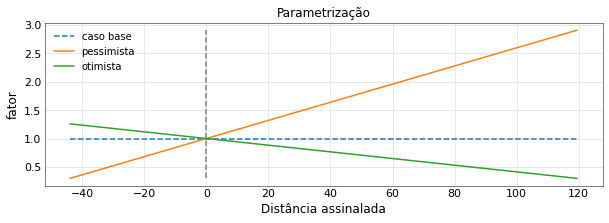
\includegraphics[width=.8\textwidth]{capitulo_2/imagens/linear_kfp.png}\label{paramlinear}} \\
     \subfloat[][Quadrática.]{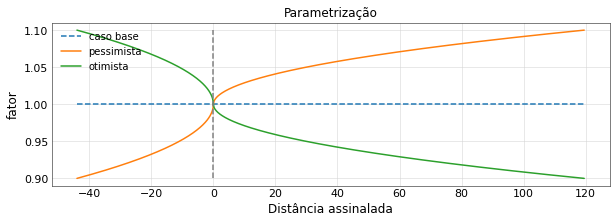
\includegraphics[width=.8\textwidth]{capitulo_2/imagens/quadratic_kfp.png}\label{paramquadrat}}
\end{figure}

\citeonline{mclennanstationarity} sugere o uso da interpolação pelo inverso da distância ao invés da krigagem porque os pesos negativos, que podem ser produzidos pela krigagem, interferem com o fator de parametrização.

\subsection{Simulação direta das distâncias assinaladas}\label{sim_direta}

\citeonline{caceres2011stochastic} e \citeonline{radtke_dissertacao} propuseram que as distâncias assinaladas sejam simuladas de forma direta: a partir de um modelo geológico implícito multi categórico, como o mostrado na \autoref{multicat_jura}, um coeficiente U de incerteza deve ser calculado de acordo com \autoref{u_eq}:

\begin{equation}\label{u_eq}
    U(u)=\frac{max\{D_{min}\}-min\{d^*_k(u)\}^K_{k=1}}{max\{D_{min}\}-min\{D_{min}\}}
\end{equation}

Onde:

\begin{equation}
    D_{min}=\{min\{d^*_k(u_1)\},...,\{min\{d^*_k(u_n)\}^K_{k=1}\}
\end{equation}

E $d^*_k(u)$ é a distância estimada no local u para a categoria k.

Os valores de U variam entre 0 e 1, um \textit{cutoff} em U determina a extensão da zona de incerteza ao redor dos contatos: quanto mais próximo de 1, mais estreita a zona. As distâncias assinaladas devem ser simuladas no interior da zona de incerteza e a categoria correspondente ao menor valor simulado é retida em cada bloco para cada realização. Os blocos simulados são concatenados com os blocos estáticos, atribuídos pela interpolação.

O método é baseado em múltiplas realizações do modelo geológico, então, seu produto final pode ser usado nas etapas posteriores do processo de avaliação. Entretanto, a metodologia tem muitos passos \cite{radtke_dissertacao}

\begin{enumerate}[label=\roman*]
\item Cálculo das distâncias assinaladas para todas as amostras e categorias;
\item Variografia das distâncias no espaço original para todas as categorias;
\item Interpolação das distâncias; 
\item criação do modelo com base na menor distância interpolada;
\item Criação da zona de incerteza;
\item Transformação Gaussiana das distâncias;
\item Variografia das distâncias no espaço gaussiano para todas as categorias;
\item Geração de múltiplos modelos baseados na menor distância simulada;
\item Validação e pós processamento das realizações.
\end{enumerate}

Além disso, a simulação é muito sensível aos parâmetros, o que muitas vezes, gera modelos com excessivo ruído, que não são geologicamente realistas, e não honram as amostras. O resultado final não justifica o número demasiado de passos e parâmetros. O coeficiente U não controla a magnitude da incerteza, apenas diminui o tempo das simulações, a magnitude da incerteza é controlada pelos parâmetros da simulação.

\subsection{Avaliação de incerteza usando imagens de treinamento para simulação multi-ponto geradas a partir dos dados}

\citeonline{silvaenhancedgeomodeling} propôs uma metodologia que integra modelagem geológica implícita com funções distâncias assinaladas e simulação geostatística multi ponto. A geostatística multi-ponto utiliza imagens de treinamento para extrair e reproduzir estruturas geológicas complexas. Geralmente, imagens de treinamento são baseadas em modelos conceituais do fenômeno geológico. Em seu trabalho, \citeonline{silvaenhancedgeomodeling} cria imagens de treinamento a partir de modelos geológicos implícitos determinísticos criados com funções distância assinaladas e modelos estocásticos criados por simulação sequencial dos indicadores. No trabalho, é introduzida uma metodologia  para integrar múltiplas imagens de treinamento, uma metodologia para calibrar a contribuição de cada imagem de treinamento e uma medida de entropia multi-ponto ao longo dos furos de sondagem.

\citeonline{silvaenhancedgeomodeling} concluiu que imagens de treinamento geradas a partir das amostras produzem modelos geológicos estocásticos, por MPS, melhores.

\subsection{Modelagem estocástica de estruturas curvilineares} 

\citeonline{lillah2013stochastic} propuseram a modelagem de estruturas curvilineares e a avaliação de incerteza desses modelos usando funções distância assinaladas. A metodologia tradicional é modificada para considerar não estacionariedade na forma de anisotropia variável localmente (LVA), que é incorporada na krigagem e na simulação sequencial Gaussiana das distâncias assinaladas. O campo de anisotropia variável captura a direção local, na qual a unidade geológica é mais contínua; enquanto, a simulação das distâncias e posterior extração da isosuperfície avalia a incerteza volumétrica.

\subsection{Avaliando e visualizando a incerteza com movimento estocástico}

\citeonline{yang2019assessing} propuseram uma técnica para avaliar e visualizar a incerteza em modelos geológicos multi-categóricos a partir do movimento estocástico. As unidades litológicas são representadas como uma soma de um modelo implícito estocástico conceitual com uma função residual condicionada às amostras e às relações cronológicas das unidades litológicas. Duas técnicas de amostragem para criação do movimento estocástico são propostas. Uma delas baseada na simulação de Monte Carlo e a outra em cadeias de Markov.

A incerteza é visualizada a partir de um filme no qual a transição entre as realizações é suave.

\subsection{Simulação dos contatos}\label{boundsim}

A metodologia proposta por \citeonline{wilde2012kriging} consiste em gerar realizações dos contatos geológicos comparando distâncias modificadas interpoladas com simulações não condicionais. 

É necessário definir, antes de qualquer coisa, uma zona de incerteza em torno dos contatos. Blocos localizados fora da zona são considerados como pertencentes a um determinado indicador, enquanto blocos dentro da zona terão sua incerteza avaliada. A zona de incerteza é obtida a partir de um parâmetro C que controla sua espessura.

A escolha do parâmetro C depende do nível de precisão requerido versus o tempo necessário para calibrar o parâmetro. Assim, o parâmetro pode ser determinado de diferentes maneiras: a determinação empírica é baseada em valores pré-determinados e/ou no conhecimento do fenômeno considerando a geometria da amostragem e a experiência do geomodelador \cite{kaperov}. A calibração parcial compara modelos interpolados com um modelo de referência. O valor de C é determinado a partir da interpretação de seções geológicas representativas e da opinião de especialistas. A calibração total é demorada e trabalhosa: são necessários vários modelos de referência para determinar o parâmetro C \cite{kaperov}. Para cada modelo de referência, um algoritmo de otimização é usado para calcular o parâmetro C, e para uma única iteração é necessário interpolar todos os modelos de referência com o mesmo parâmetro C. Para alcançar a calibração completa, várias iterações são necessárias usando valores diferentes para o parâmetro C, que demanda um grande esforço computacional e aumenta o tamanho e o número dos modelos de referência usados \cite{munroe2008full}.

A calibração também pode ser realizada por um método semelhante à metodologia de validação cruzada por \textit{jackknife} \cite{wilde2012kriging}, utilizando apenas os dados para calibrar o parâmetro C com baixa demanda computacional e alta automatização.

O primeiro passo na calibração de C por \textit{jackknife} é remover um subconjunto dos dados. Isso pode ser feito escolhendo aleatoriamente os furos de sondagem a serem excluídos. Um estudo de calibração adequado envolve a geração de vários conjuntos, com diferentes proporções (50\% a 10\%) e diferentes configurações de dados removidos \cite{manchuck}. Os valores da função distância são então calculados para os dados restantes com um valor inicial para C igual a zero. Essas amostras da função distância assinaladas são usadas para condicionar a estimativa da função distância em cada um dos locais de dados removidos. Existem quatro resultados possíveis  desta estimativa. A localização pode ser: corretamente estimada como fora do domínio, corretamente estimada como dentro do domínio, incorretamente estimada como fora do domínio e incorretamente estimada como dentro do domínio. O principal interesse está no número de dados que caem do lado errado da fronteira, ou seja, o número de vezes que a estimativa é positiva, mas os dados são codificados como dentro do domínio e o número de vezes que a estimativa é negativa, mas o os dados são codificados como fora do domínio. O número de vezes que um dado cai do lado errado do limite para C igual a zero é o caso base.

O valor de C é então aumentado e os valores da função distância das amostras não removidas são modificados de acordo com a \autoref{C_dist}. Essa função distância modificada é estimada nos locais das amostras removidas. O limite agora é considerado como estando entre -C e C. Os dados caem do lado errado do limite quando um local estimado é codificado como interno, mas tem uma estimativa para a função distância modificada maior que C ou um local estimado é codificado como externo, mas tem uma estimativa da função distância modificada menor que -C. O número de dados que caem do lado errado do limite diminui à medida que C aumenta. C é aumentado até que o número de dados que caem no lado errado do limite seja aceitável. O valor C onde isso ocorre é o valor C calibrado que quantifica a incerteza do limite.

\begin{equation}
	d_k(u_\alpha)=\begin{cases}
	-\parallel u_\alpha-u_\beta\parallel - C,\:\textrm{se $u_\alpha$ pertence ao domínio}\\
	+\parallel u_\alpha-u_\beta\parallel + C,\:\textrm{se $u_\alpha$ não pertence ao domínio}\end{cases}
    \label{C_dist}
\end{equation}

A \autoref{c_uncert} mostra, para um esquema sintético em duas dimensões, em branco a zona considerada fora domínio, em preto dentro do domínio e em cinza a zona de contato para diferentes valores de C. À medida que C aumenta, o número de classificações errôneas diminui já que qualquer ponto estimado na zona cinza não é uma classificação errônea. Os sinais (+ e -) representam as amostras e sua distância assinalada calculada.

\begin{figure}[H]
	\caption{\label{c_uncert}Calibração do parâmetro C para um esquema em duas dimensões.}
	\centering
		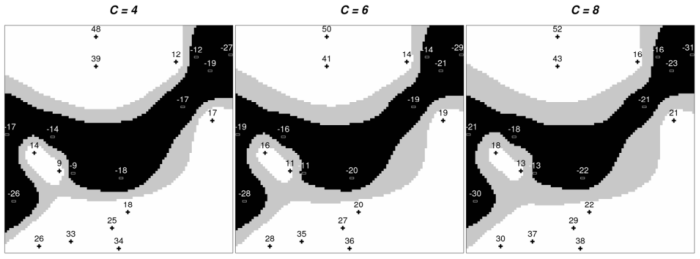
\includegraphics[width=0.8\textwidth]{capitulo_2/imagens/c_uncert.png}
	\legend{Fonte: \citeonline{wilde2012kriging}}
\end{figure}

Uma curva como a da \autoref{c_calib_grafico} é construída. São escolhidos N valores para C entre zero e um valor definido pelo usuário (linhas tracejadas em verde). Para cada um desses valores de C, são removidos X\% dos furos (ou amostras em duas dimensões) Z vezes (estrelas azuis). É indicado que a classificação errônea seja calculada diversas vezes para que a calibração de C seja robusta \cite{wilde2012kriging}. O índice de classificação errônea é registrado no eixo Y do gráfico (estrelas azuis) e o valor de C no eixo X (linhas tracejadas em verde). Então traça-se a classificação errônea média (curva em preto).

\begin{figure}[H]
	\caption{\label{c_calib_grafico}Figura esquemática da curva de calibração.}
	\centering
		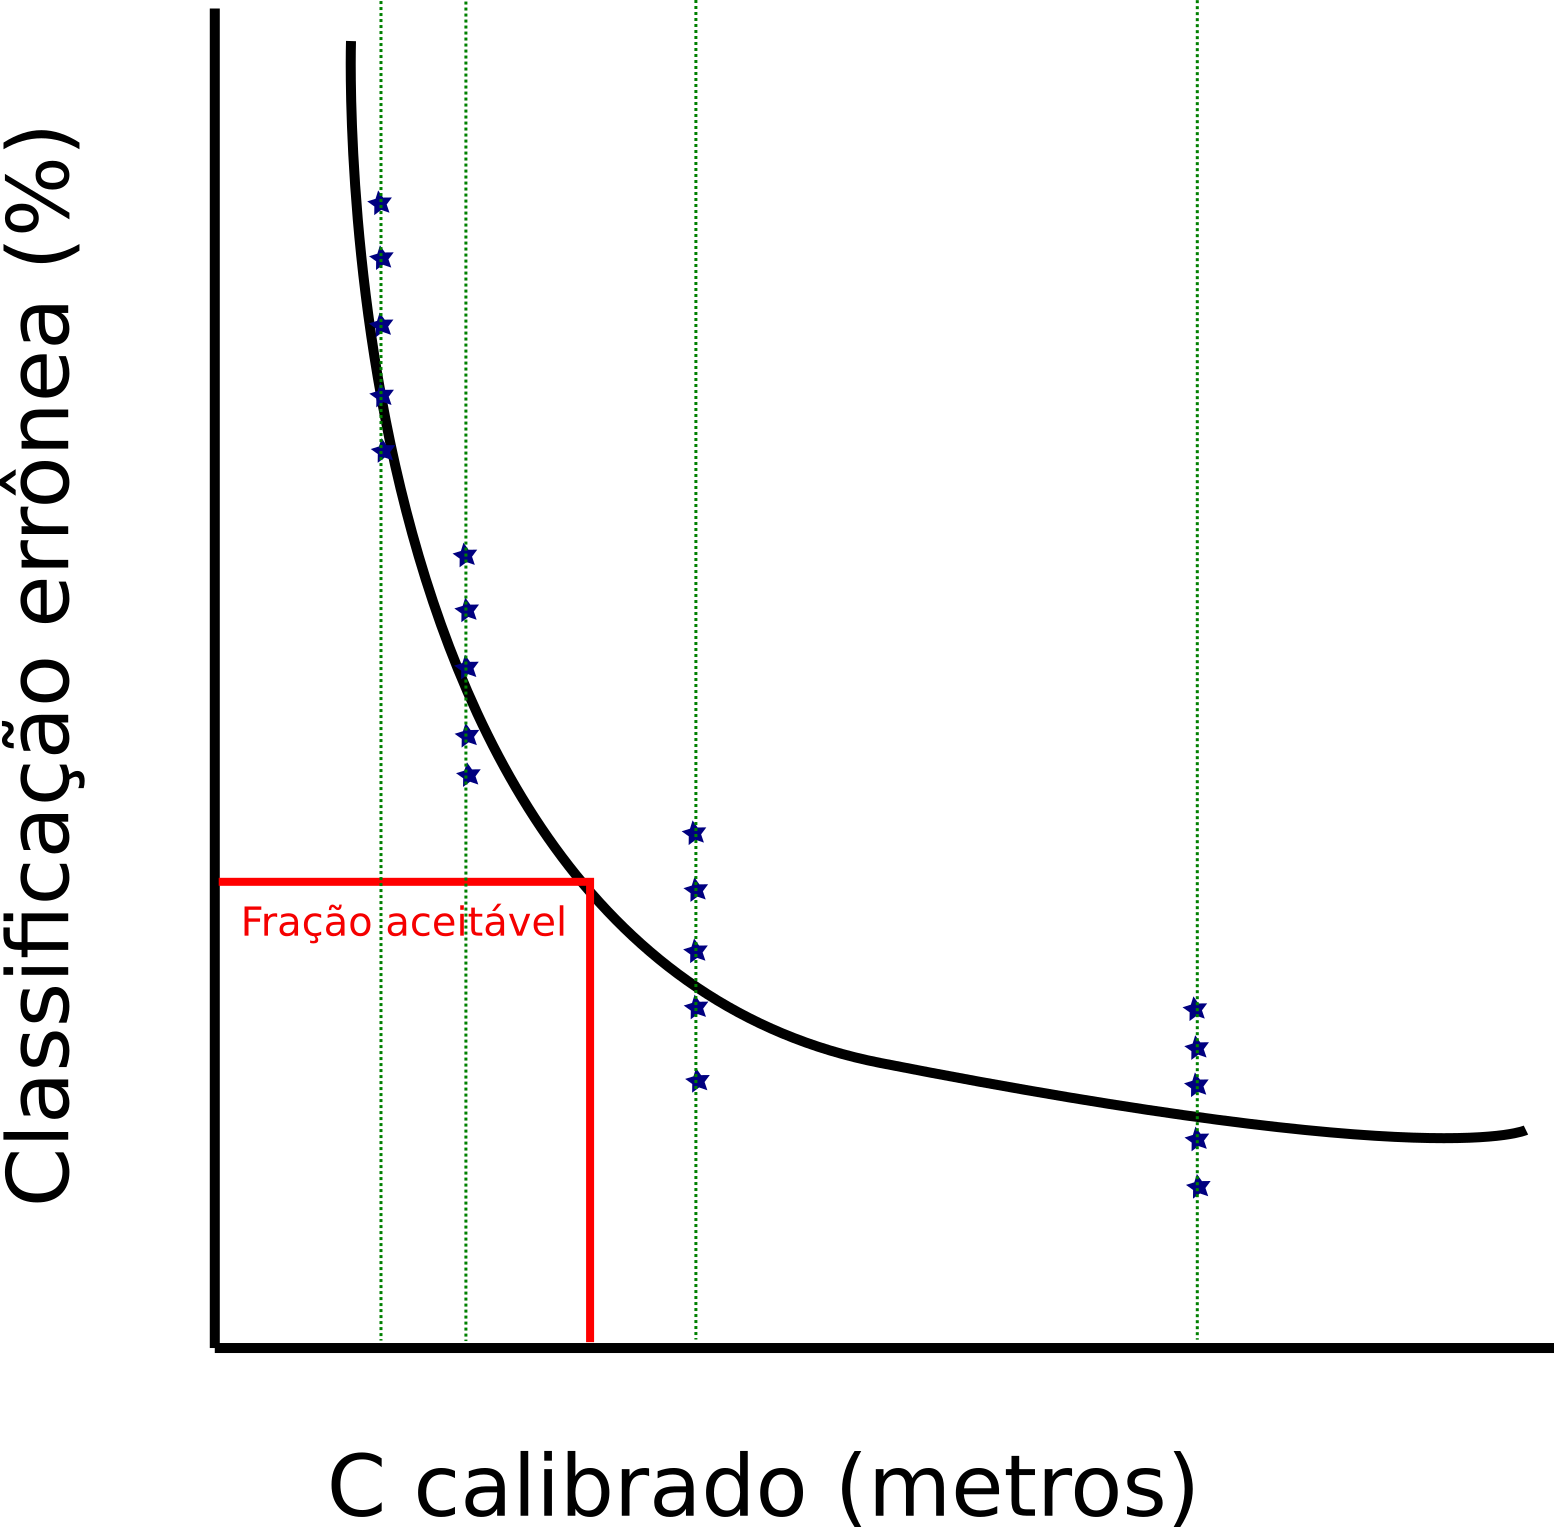
\includegraphics[width=0.6\textwidth]{capitulo_2/imagens/calibration.png}
\end{figure}

\citeonline{manchuck_deutsch_Geometric} sugerem 2,5\% de classificação errônea um nível aceitável para depósitos tabulares, \cite{martin2017implicitmodeling} definiram como 3.9\% para um dos domínios de um depósito de cobre. Uma outra forma de escolha é o método do cotovelo, o valor tomado deve ser o ponto de inflexão da curva de calibração \cite{martin2017implicitmodeling}. C depende do tipo de depósito e da configuração geométrica das amostras. Para depósitos com menor variabilidade, como os de bauxita por exemplo, C deve ser pequeno. Já para depósitos com maior variação, como os de ouro, o valor de C deve ser maior. Para amostragens densas o valor de C deve ser menor em relação à amostragens esparsas. C não deve ser maior do que a malha de sondagem.

Após o valor de C ser selecionado, as distâncias assinaladas calculadas para cada amostra devem ser modificadas a partir da equação \autoref{C_dist}. As distâncias modificadas devem então ser interpoladas, utilizando o mesmo variograma das distâncias originais, para todos os nós do \textit{grid}, e a truncagem das distâncias modificadas estimadas entre -C e +C define a zona de incerteza.

Valores para a função distância são simulados uniformemente entre -C e +C. Para isso, é necessário realizar uma simulação Gaussiana não condicional. Um dos algoritmos comumente usados é a simulação sequencial Gaussiana (\autoref{algo:usgs}). O variograma utilizado na simulação não condicional pode ser o mesmo das distâncias assinaladas. O alcance do variograma determina a natureza do contato entre os domínios, menores alcances geram contatos mais rugosos enquanto maiores alcances, contatos suaves. O efeito pepita controla a inter conectividade entre o domínio.

\begin{algorithm}
\SetAlgoLined
    1. Defina um caminho aleatório através dos nós do \textit{grid}\;
    \For{cada nó}{
    1. Busque no espaço por nós previamente simulados\;
    \eIf{número de nós previamente simulados != 0}{
    1. Construa e resolva o sistema de krigagem\;
    2. Amostre a distribuição condicional construída a partir da média e da variância\;
    }{
    1. Amostre a partir de uma distribuição Gaussiana padrão\;
    }
    2. Atribua o valor amostrado ao nó do modelo e inclua o nó simulado no conjunto de dados simulado anteriormente\;
    }
 \caption{Simulação sequencial Gaussiana não condicional}\label{algo:usgs}
\end{algorithm}

Para que os valores simulados se distribuam de forma uniforme entre –C e +C, o valor Gaussiano, deve ser transformado pela relação:

\begin{equation}
\label{sim_trans}
    df'(u)=2*C*G^-1(y'(u))-C
\end{equation}

Onde: $df'(u)$ é o valor da função distância simulada, $y'(u)$ o valor normal padrão da simulação não condicional, e $G^-1$ representa a determinação do valor da distribuição acumulada padrão normal correspondente a $y'(u)$. Para garantir que os valores pertençam a região estabelecida os valores são multiplicados por 2C e subtraídos de C.

A \autoref{sim_zona_c} mostra duas realizações da simulação das distâncias para uma zona de incerteza igual a 5 metros para o esquema em duas dimensões da \autoref{c_uncert}.

\begin{figure}[H]
	\caption{\label{sim_zona_c}Simulação das distâncias dentro da zona de incerteza para um esquema em duas dimensões.}
	\centering
		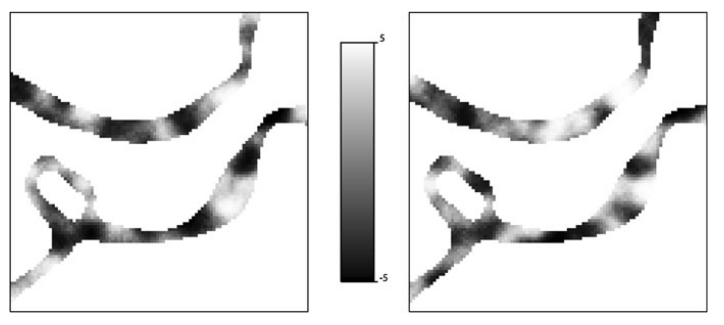
\includegraphics[width=0.8\textwidth]{capitulo_2/imagens/sim_zona_c.png}
	\legend{Fonte: \citeonline{wilde2012kriging}}
\end{figure}

Os contatos podem agora ser simulados no interior da zona de incerteza. Caso o valor interpolado $df^{*}(u)$ seja menor que o valor simulado $df'(u)$ para a função distância, o local é considerado pertencente ao domínio (indicador 1), caso o valor interpolado seja maior que o simulado, o local é considerado externo ao domínio (indicador 0), como evidenciado pela \autoref{comp_class}. Nos locais onde a interpolação apresenta o mesmo valor da simulação, são estabelecidos os contatos dos domínios como esquematizado na \autoref{conceptual}.

\begin{equation}
\label{comp_class}
	i`(u)=\begin{cases}
	indicador \: 1, \: se \: df'(u) > df^{*}(u)\\
	indicador \: 0, \: se \: df'(u) < df^{*}(u)\end{cases}
\end{equation}

\begin{figure}[H]
	\caption{\label{conceptual}Esquema mostrando como os contatos são simulados dentro da zona de incerteza.}
	\centering
		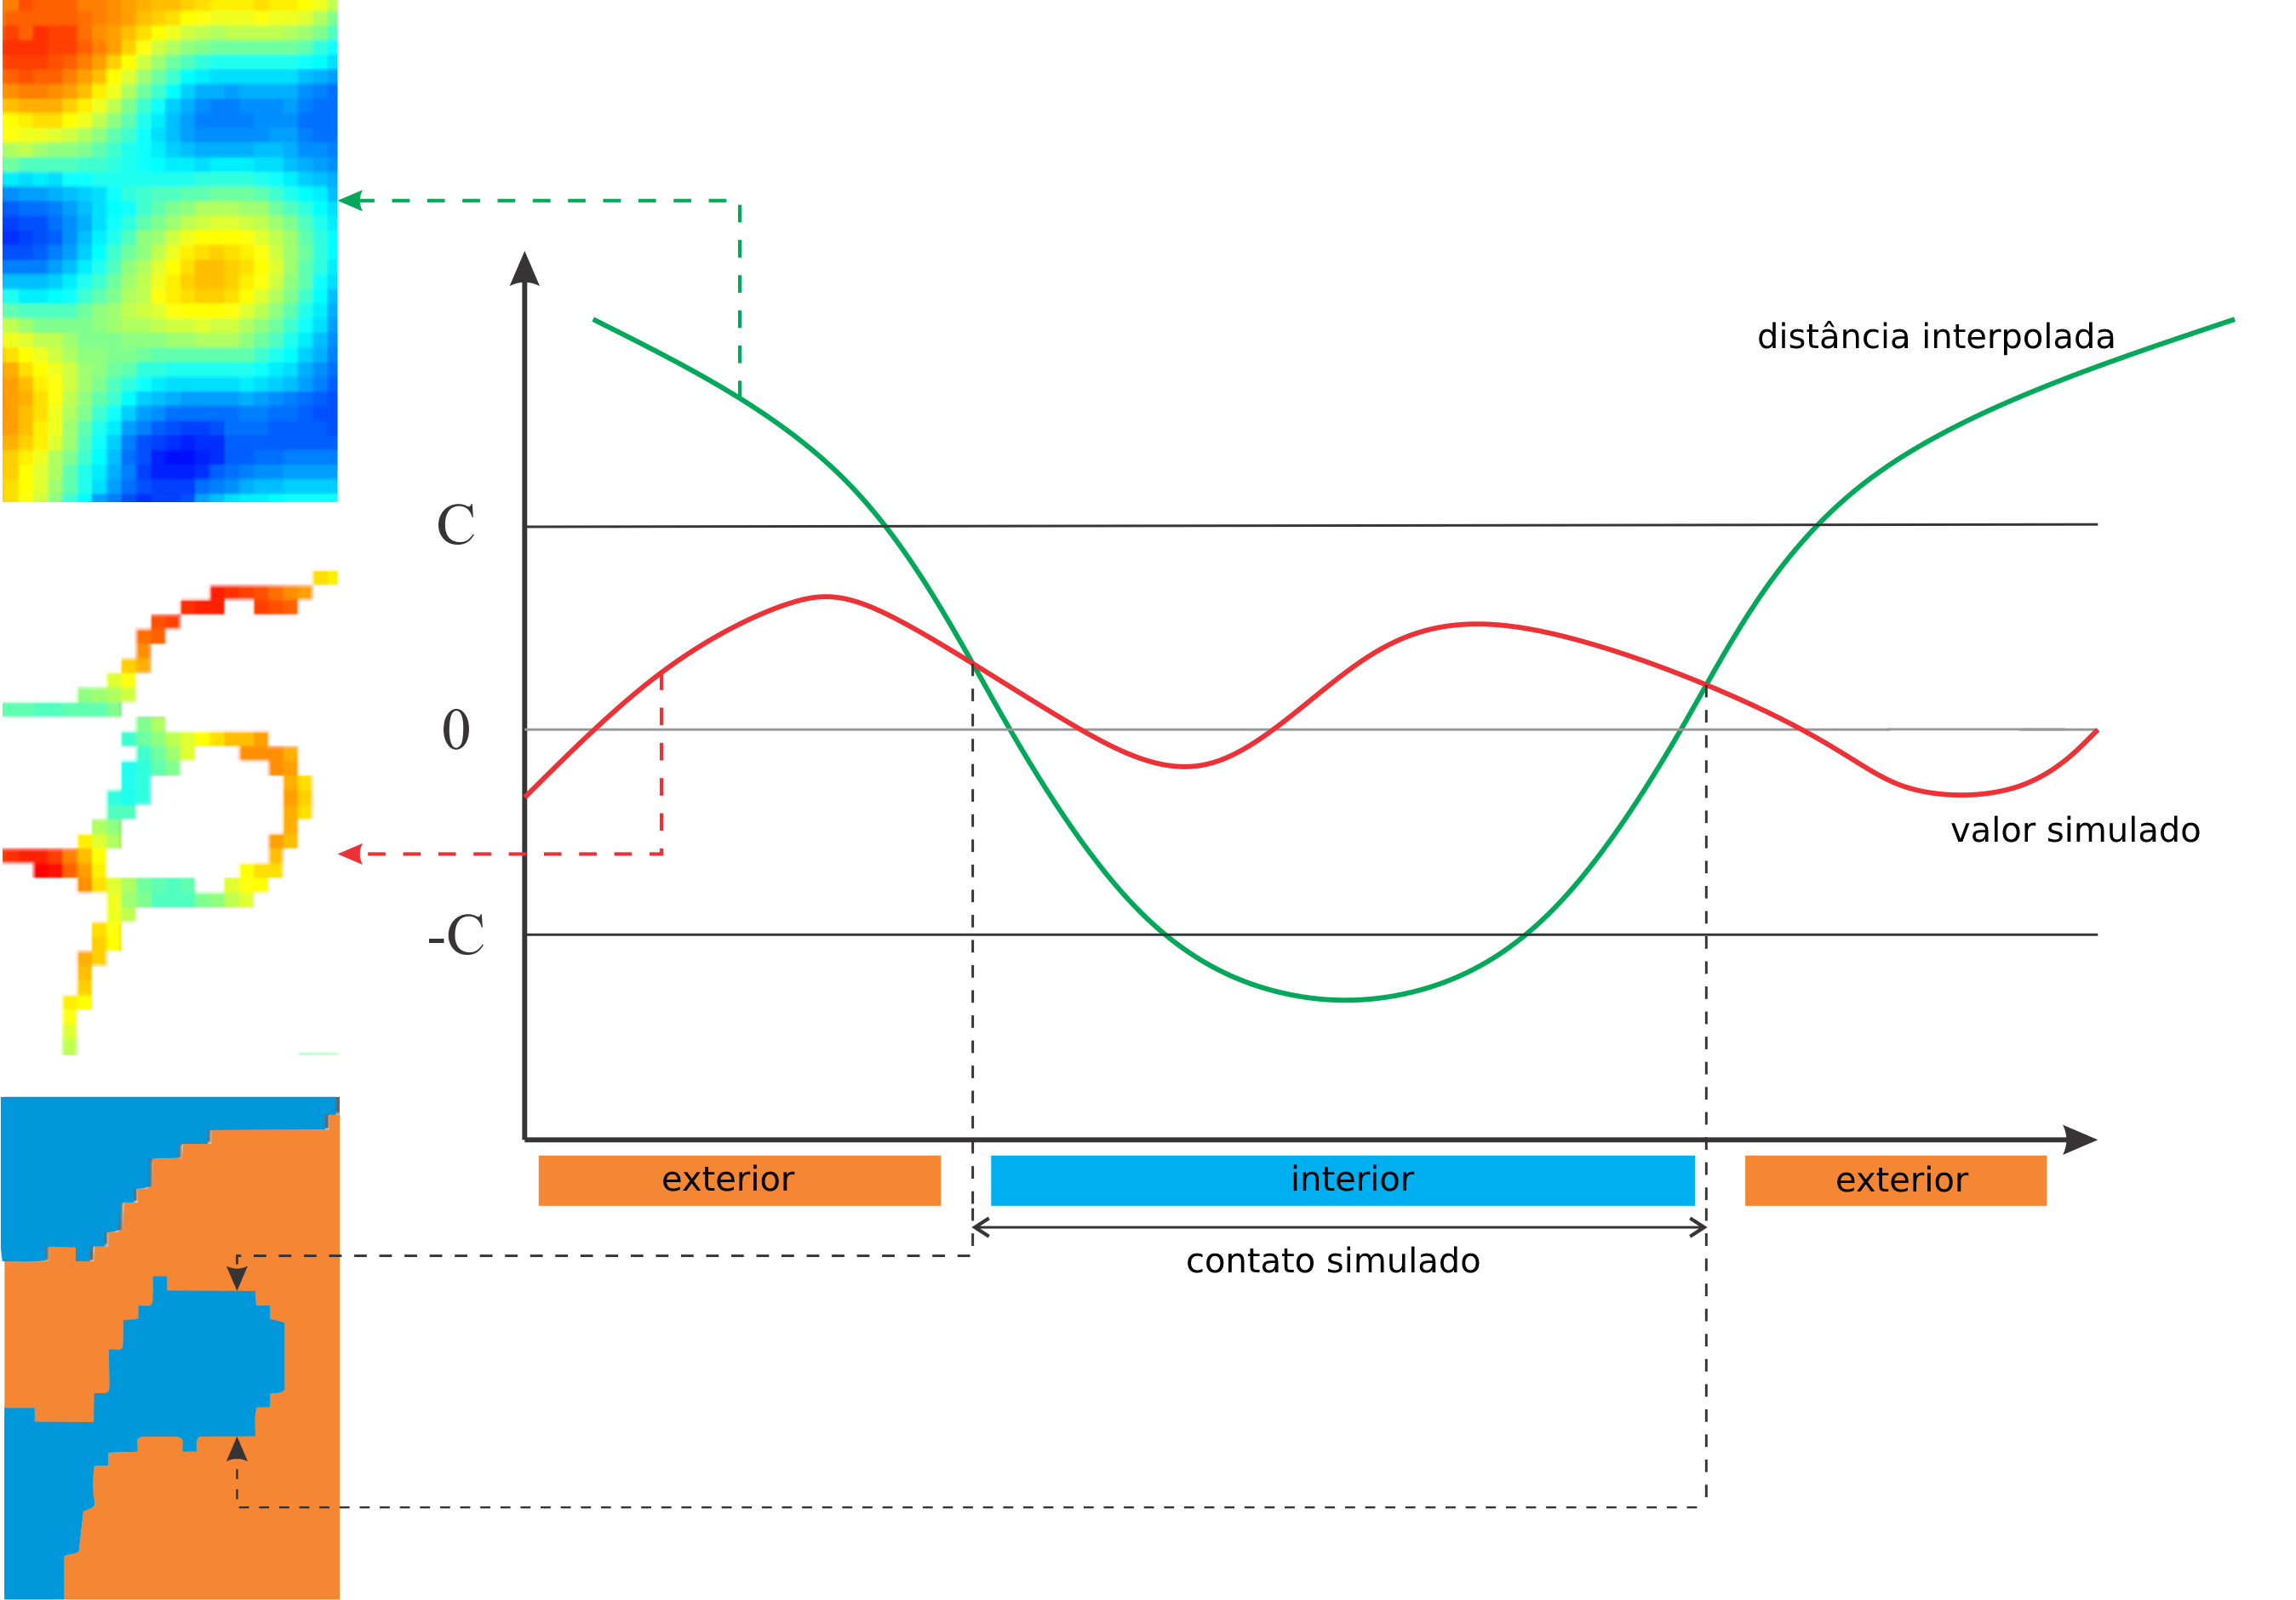
\includegraphics[width=\textwidth]{capitulo_2/imagens/conceptual.png}
		\legend{Modificado de \citeonline{amarante2021boundary}}
\end{figure}

A \autoref{final_result} mostra duas diferentes realizações da simulação dos contatos para o esquema em duas dimensões mostrado na \autoref{c_uncert}.

\begin{figure}[H]
	\caption{\label{final_result}Duas realizações da simulação dos contatos para um esquema em duas dimensões.}
	\centering
		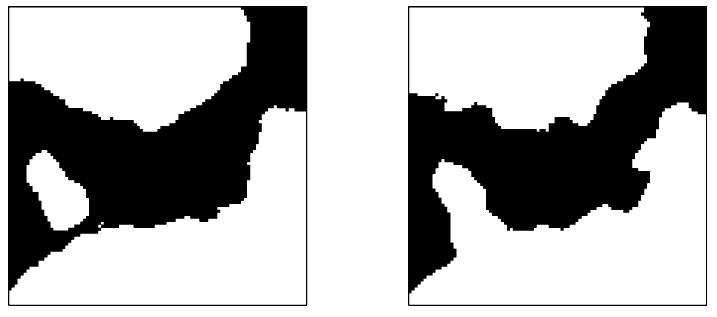
\includegraphics[width=0.8\textwidth]{capitulo_2/imagens/final result.png}
	\legend{Fonte: \citeonline{wilde2012kriging}}
\end{figure}

O método é rápido, já que é baseado em simulações não condicionais, gera modelos realista,s sem ruído e com fronteiras contínuas. Tanto a magnitude da incerteza, quanto a natureza da fronteira podem ser controlados. Entretanto, o método funciona apenas para uma categoria por vez e mesmo que simplificações tenham sido desenvolvidas, a calibração do parâmetro de incerteza ainda pode ser laboriosa e subjetiva.